
% ---------------------------------------------------------------------------- %
%                              DOCUMENT DEFINITION                             %
% ---------------------------------------------------------------------------- %

% --- 문서 스타일 정의 ---
\documentclass[oneside,openany,a4paper,12pt]{book}
% ---------------------------------------------------------------------------- %
%                                   PACKAGES                                   %
% ---------------------------------------------------------------------------- %

% --- 한글 및 기본 설정 패키지 ---
\usepackage{kotex}                     % 한글 지원
\usepackage{graphicx}                  % 그림 포함
\usepackage{xcolor}                    % 색상 지원

% --- 제목/번호/목차 관련 ---
\usepackage{titling}                   % 커스텀 표지 지원
\usepackage{titlesec}                  % 제목 포맷 커스텀
\usepackage{setspace}                  % 줄간격 조정
\setstretch{1.5}                       % 기본 줄간격 1.5배
\setlength{\parskip}{0.6em}            % 단락 사이 간격
\setlength{\parindent}{1em}            % 단락 들여쓰기

% --- 수식 및 수학 패키지 ---
\usepackage{amsmath}                   % 수학 공식
\numberwithin{equation}{chapter}       % 챕터별 수식번호

% --- 표, 그림 관련 패키지 ---
\usepackage{booktabs}                  % \toprule 등 고급 표
\usepackage{longtable}                 % 페이지 나누는 표
\usepackage{tabularx}                  % 가변 폭 표
\usepackage{multirow}                  % 셀 병합
\usepackage{makecell}
\usepackage[tableposition=top]{caption}% 표 캡션 위 고정
\usepackage{subcaption}
\usepackage{array}
\newcolumntype{Y}{>{\centering\arraybackslash}X}

% --- 기타 디자인 ---
\usepackage[most]{tcolorbox}                 % 박스 디자인

% --- 레이아웃, 그림폴더 등 ---
\usepackage[margin=2cm,headheight=1cm]{geometry}
\graphicspath{{./_figures/}}

% --- 코드류 ---
\usepackage{listings}
\usepackage{ifthen}

% --- 주석 --- 
\usepackage{todonotes}

% --- 링크 ---
\usepackage[colorlinks, linkcolor=blue, citecolor=red]{hyperref} % 하이퍼링크
\usepackage[capitalise]{cleveref}      % cref 레퍼런스
\hypersetup{
  pdftitle={시뮬레이터 기술문서},
  pdfauthor={서울대학교 건축에너지연구실},
  pdfkeywords={},
  bookmarksopen=true
}
% ---------------------------------------------------------------------------- %
%                                   SETTINGS                                   %
% ---------------------------------------------------------------------------- %

% --- 목차, 그림/표목차, 참고문헌 등 한글화 ---
\renewcommand{\contentsname}{목차}
\renewcommand{\listfigurename}{그림 목록}
\renewcommand{\listtablename}{표 목록}
\renewcommand{\bibname}{참고문헌}

% --- 그림, 표, 식, 장, 절 인용 표기 --- 
\crefname{figure}{그림}{그림}
\Crefname{figure}{그림}{그림}
\crefname{table}{표}{표}
\Crefname{table}{표}{표}
\crefname{equation}{식}{식}
\Crefname{equation}{식}{식}
% \crefname{chapter}{장}{장}  % 밑에 crefformat이 오버라이딩해서 없어도 될듯
\crefformat{chapter}{#2#1장#3}
\crefformat{section}{#2#1절#3}
\crefformat{subsection}{#2#1절#3}

% --- secnum, 제목 스타일, 단락 스타일 등 ---
\setcounter{secnumdepth}{3}            % subsubsection까지 번호 매김

% --- part 스타일 ---
\titleformat{\part}
  {\centering\Huge\bfseries}
  {\thepart}
  {0pt}
  {
    \thispagestyle{empty}
  }

% --- chapter 스타일: 본문과 appendix에 따라 변경 가능하게 ---
\newcommand{\chapterlabel}{제\thechapter 장}
\titleformat{\chapter}[hang]
  {\normalfont\huge\bfseries}
  {\chapterlabel}
  {1em}
  {}

% --- paragraph, subparagraph 스타일 ---
\titleformat{\paragraph}[runin]
  {\normalfont\itshape\bfseries}
  {\theparagraph}{1em}{}
\titleformat{\subparagraph}[runin]
  {\normalfont\itshape\bfseries}
  {\thesubparagraph}{1em}{}

% --- 메모 스타일 ---
\definecolor{gonie_color}{RGB}{255, 255, 180}  
\definecolor{hongI_color}{RGB}{200, 255, 200} 
\definecolor{theungDu_color}{RGB}{176, 224, 230}   
\definecolor{형진_color}{RGB}{255, 220, 230}   

\let\originaltodo\todo
\renewcommand{\todo}[2]{%
  \ifthenelse{\equal{#1}{형곤}}%
    {\originaltodo[color=gonie_color, size=tiny]{\textbf{#1}: #2}}%
  {%
  \ifthenelse{\equal{#1}{철홍}}%
    {\originaltodo[color=hongI_color, size=tiny]{\textbf{#1}: #2}}%
  {%
  \ifthenelse{\equal{#1}{승주}}%
    {\originaltodo[color=theungDu_color, size=tiny]{\textbf{#1}: #2}}%
  {%
  \ifthenelse{\equal{#1}{형진}}%
    {\originaltodo[color=형진_color, size=tiny]{\textbf{#1}: #2}}%
  {%
    \originaltodo[color=gray!20, size=tiny]{\textbf{#1}: #2} % 기본값
  }}}}%
}
% ---------------------------------------------------------------------------- %
%                                     STYLE                                    %
% ---------------------------------------------------------------------------- %

% --- 그림, 표 환경 커스텀 ---
\newenvironment{defaultfigure}
  {%
  \vspace{0.3em}
  \begin{figure}[htbp]\centering
    \setlength{\belowcaptionskip}{0.3em}
  }
  {\end{figure}}

\renewcommand{\arraystretch}{1.5}
\newenvironment{defaulttable}
  {\begin{table}[htbp]\centering\small}
  {\end{table}}

\newenvironment{variabletable}
  {\begin{defaulttable}}
  {\end{defaulttable}}

% 단위 표시
\newcommand{\unitsty}[1]{{\small $#1$}}
% ---------------------------------------------------------------------------- %
%                                     NAMES                                    %
% ---------------------------------------------------------------------------- %

% --- release 관련 정보 (변수형) ---
\newcommand{\releaseversion}{0-4-5-1}
\newcommand{\releasedate}{2025.09.25.}


% --- 반복되는 용어/alias 정의 ---
\newcommand{\ep}{EnergyPlus}
\newcommand{\simulator}{EPlusSimple}

\newcommand{\pymodule}{epsimple}
\newcommand{\unit}[1]{
  \begingroup
  \ifthenelse{\equal{#1}{density}}{$kg/m^3$}{%
  \ifthenelse{\equal{#1}{conductivity}}{$W/mK$}{%
  \ifthenelse{\equal{#1}{U}}{$W/m^2K$}{-}}}
  \endgroup
}

% --- 

% --- 문서 시작 ---
\begin{document}
\pagestyle{plain} 

% ---------------------------------------------------------------------------- %
%                                 PRELIMINARIES                                %
% ---------------------------------------------------------------------------- %

\listoftodos

% --- 표지 ---
\begin{titlepage}
  \centering
  % 제목 및 상단 문구
  {\scshape\large \simulator Version 0.2.0 Documentation\par}
  \vspace{6em}
  {\bfseries\Huge Program Manual and 이것저것 test\par}
  \vspace{1em}
  {\itshape\Large Korea Authority of Land \& Infrastructure Safety\par}
  {\itshape\Large Seoul National University\par}
  {\itshape\Large Super-Duper Invisible Dragon\par}
  \vfill
  % 중앙 그림 (로고)
  
\includegraphics[height=0.25\textwidth]{국토안전관리원_시그니처2.png}
  \hspace{2em}
  
\includegraphics[height=0.25\textwidth]{snu_ui.png}
  \hspace{2em}
  
\includegraphics[height=0.25\textwidth]{my_tiny_dragon.png}
  \vfill
  % 하단
  {\large \today \par}
  \vspace{0.5em}
  {\small COPYRIGHT (c) 이 도구는 국토부, 안전원의 후원을 받아... 서울대가 열심히 사부작 사부작...}
\end{titlepage}

% --- 서문 ---
\section*{서문}
본 문서는 high-fidelity 동적에너지 시뮬레이션에 기반한 그린리모델링 의사결정 지원 도구, \simulator 프로그램(Version\simulatorversion)의 사용법 및 입력 방식을 기술한 문서로, 본 엔진을 이용하여 retrofit 의사결정을 하고자 하는 연구자, ..공무원 ..... 를 위해 작성되었습니다.

본 문서는 아래와 같은 순서로 기술되어 있습니다.
\begin{itemize}
  \item 제1부[개요]에서는, 본 프로그램의 가이드라인에 대한 개요를 기술합니다.
  \item 제2부[프로그램 시작]에서는, 본 시뮬레이터의 설치 및 실행 방법에 대하여 기술합니다.
  \item 제3부[입력 요령]에서는, 기축 건물의 정보를 시뮬레이터에 입력하는 요령에 대하여 기술합니다.
  \item 제4부[Python 모듈 개발]에서는, 본 엔진을 위해 개발된 \pymodule의 개발 과정 및 구조, 사용법에 대하여 기술하고, 모듈의 수정 등 유지보수를 위한 가이드를 기술합니다.
  \item 제5부[혹시몰라쓸거있나]에서는, 안하고시펑.
  \item 마지막으로 부록에서는, 본 엔진을 개발함에 있어 의사결정의 근거가 되었던 각종 실험 결과 등에 대하여 기술합니다.
  \item 얼마나 빠른지 보자
  \item 어떻게 하는거임 도당체
  \item 태그 기능 테스트
\end{itemize}

% --- 목차 ---
\pagenumbering{roman}
\tableofcontents       
\listoffigures          
\listoftables          

% ---------------------------------------------------------------------------- %
%                                  MAINMATTER                                  %
% ---------------------------------------------------------------------------- %

% --- 페이지 초기화 ---
\clearpage      
\pagenumbering{arabic}

% --- 본문 ---
\mainmatter
% chap1.tex
\part{서론}
\label{part:introduction}

% ---------------------------------------------------------------------------- %
%                                  NEW SECTION                                 %
% ---------------------------------------------------------------------------- %

\chapter{개발 배경 및 원리}

\section{동적 시뮬레이션 기반 그린리모델링 의사결정 지원도구}

 그린리모델링은 기술간의 교호작용을 고려할 수 있는 동적 시뮬레이션 도구가 필요하다.
 하지만 EnergyPlus는 ...하여 그린리모델링 사업에서 실제로 쓰이기에는 부적합하기 때문에, ...한 시뮬레이터가 요구된다.

% ---------------------------------------------------------------------------- %
%                                  NEW SECTION                                 %
% ---------------------------------------------------------------------------- %

\section{\simulator의 접근 및 철학}

\subsection{원칙}
ECO2 입력 수준 만큼의 노력으로 high-fidelity 동적 시뮬레이션 가능하게 하는 걸 목적으로 하여, 아래 원칙 하에서 개발하였다.

\begin{itemize}
  \item 기존에 국내에서 쓰이던 건물 에너지 평가 도구의 입력 수준과 유사
  \item EnergyPlus 엔진을 사용하여 건물의 동적 거동 상세하게 모사
  \item 기축건물에서 사용자가 얻기 어렵지만, 동적 시뮬레이터에서 요구하는 것들 가정 (normative dynamic)
  \item ASHRAE F., 건축물에너지효율등급인증규정 등 국내외 기준 참고하여 표준적인 시뮬레이션이 가능
\end{itemize}

\subsection{다른 도구들과의 관계}
\subsubsection{EnergyPlus, DesignBuilder}
\simulator\는 EnergyPlus의 wrapper로 볼 수 있다. EnergyPlus는 엔진의 역할, DesignBuilder가 그걸 포장하는 툴인데, \simulator~도 비슷한 관점에서 개발되었다. 단, DesignBuilder는 높은 자유도를 거의 그대로 보장하고 사용 가능한 dataset도 그냥 열린 반면에, \simulator\는 국내 실정과 기축건물의 그린리모델링이라는 상황에 적합하게 커스터마이징하여, 그린리모델링 사업에 적합하게 사용 가능하다.

\subsubsection{ClimateStudio, Honeybee}
둘 다 EnergyPlus의 앞서 언급한 DesignBuilder와 같은 wrapper인데, Raw-level에서의 수정도구인 DesignBuilder보다는 좀 더 graphical code 개념도 쓰고 해서 좀 더 구조적인 모델링이 가능하다. \simulator~의 자료구조와 python 코드상의 구조는 두 프로그램의 자료구조를 참고하여 개발되었다.

\subsubsection{ECO2(-OD)}
\simulator\는 ECO2의 입력 수준을 많이 넘지 않는 것을 원칙으로 하고 있기 때문에, 입력변수의 종류와 그 상세함의 정도는 ECO2 및 ECO2-OD를 참고하여 결정하였다. 특히 실 단위 부하를 계산하는 ECO2의 데이터베이스 등을 많이 참고하였다.

% ---------------------------------------------------------------------------- %
%                                  NEW SECTION                                 %
% ---------------------------------------------------------------------------- %

\section{\simulator의 개요 및 역할}

\simulator\는 사용자의 간단한 입력데이터를 \ep 실행이 가능한 형태로 변환하는 도구로 이해할 수 있다 (그림 \ref{fig:package_function}). 그 변환 과정은 python이 매개한다.

\begin{defaultfigure}
  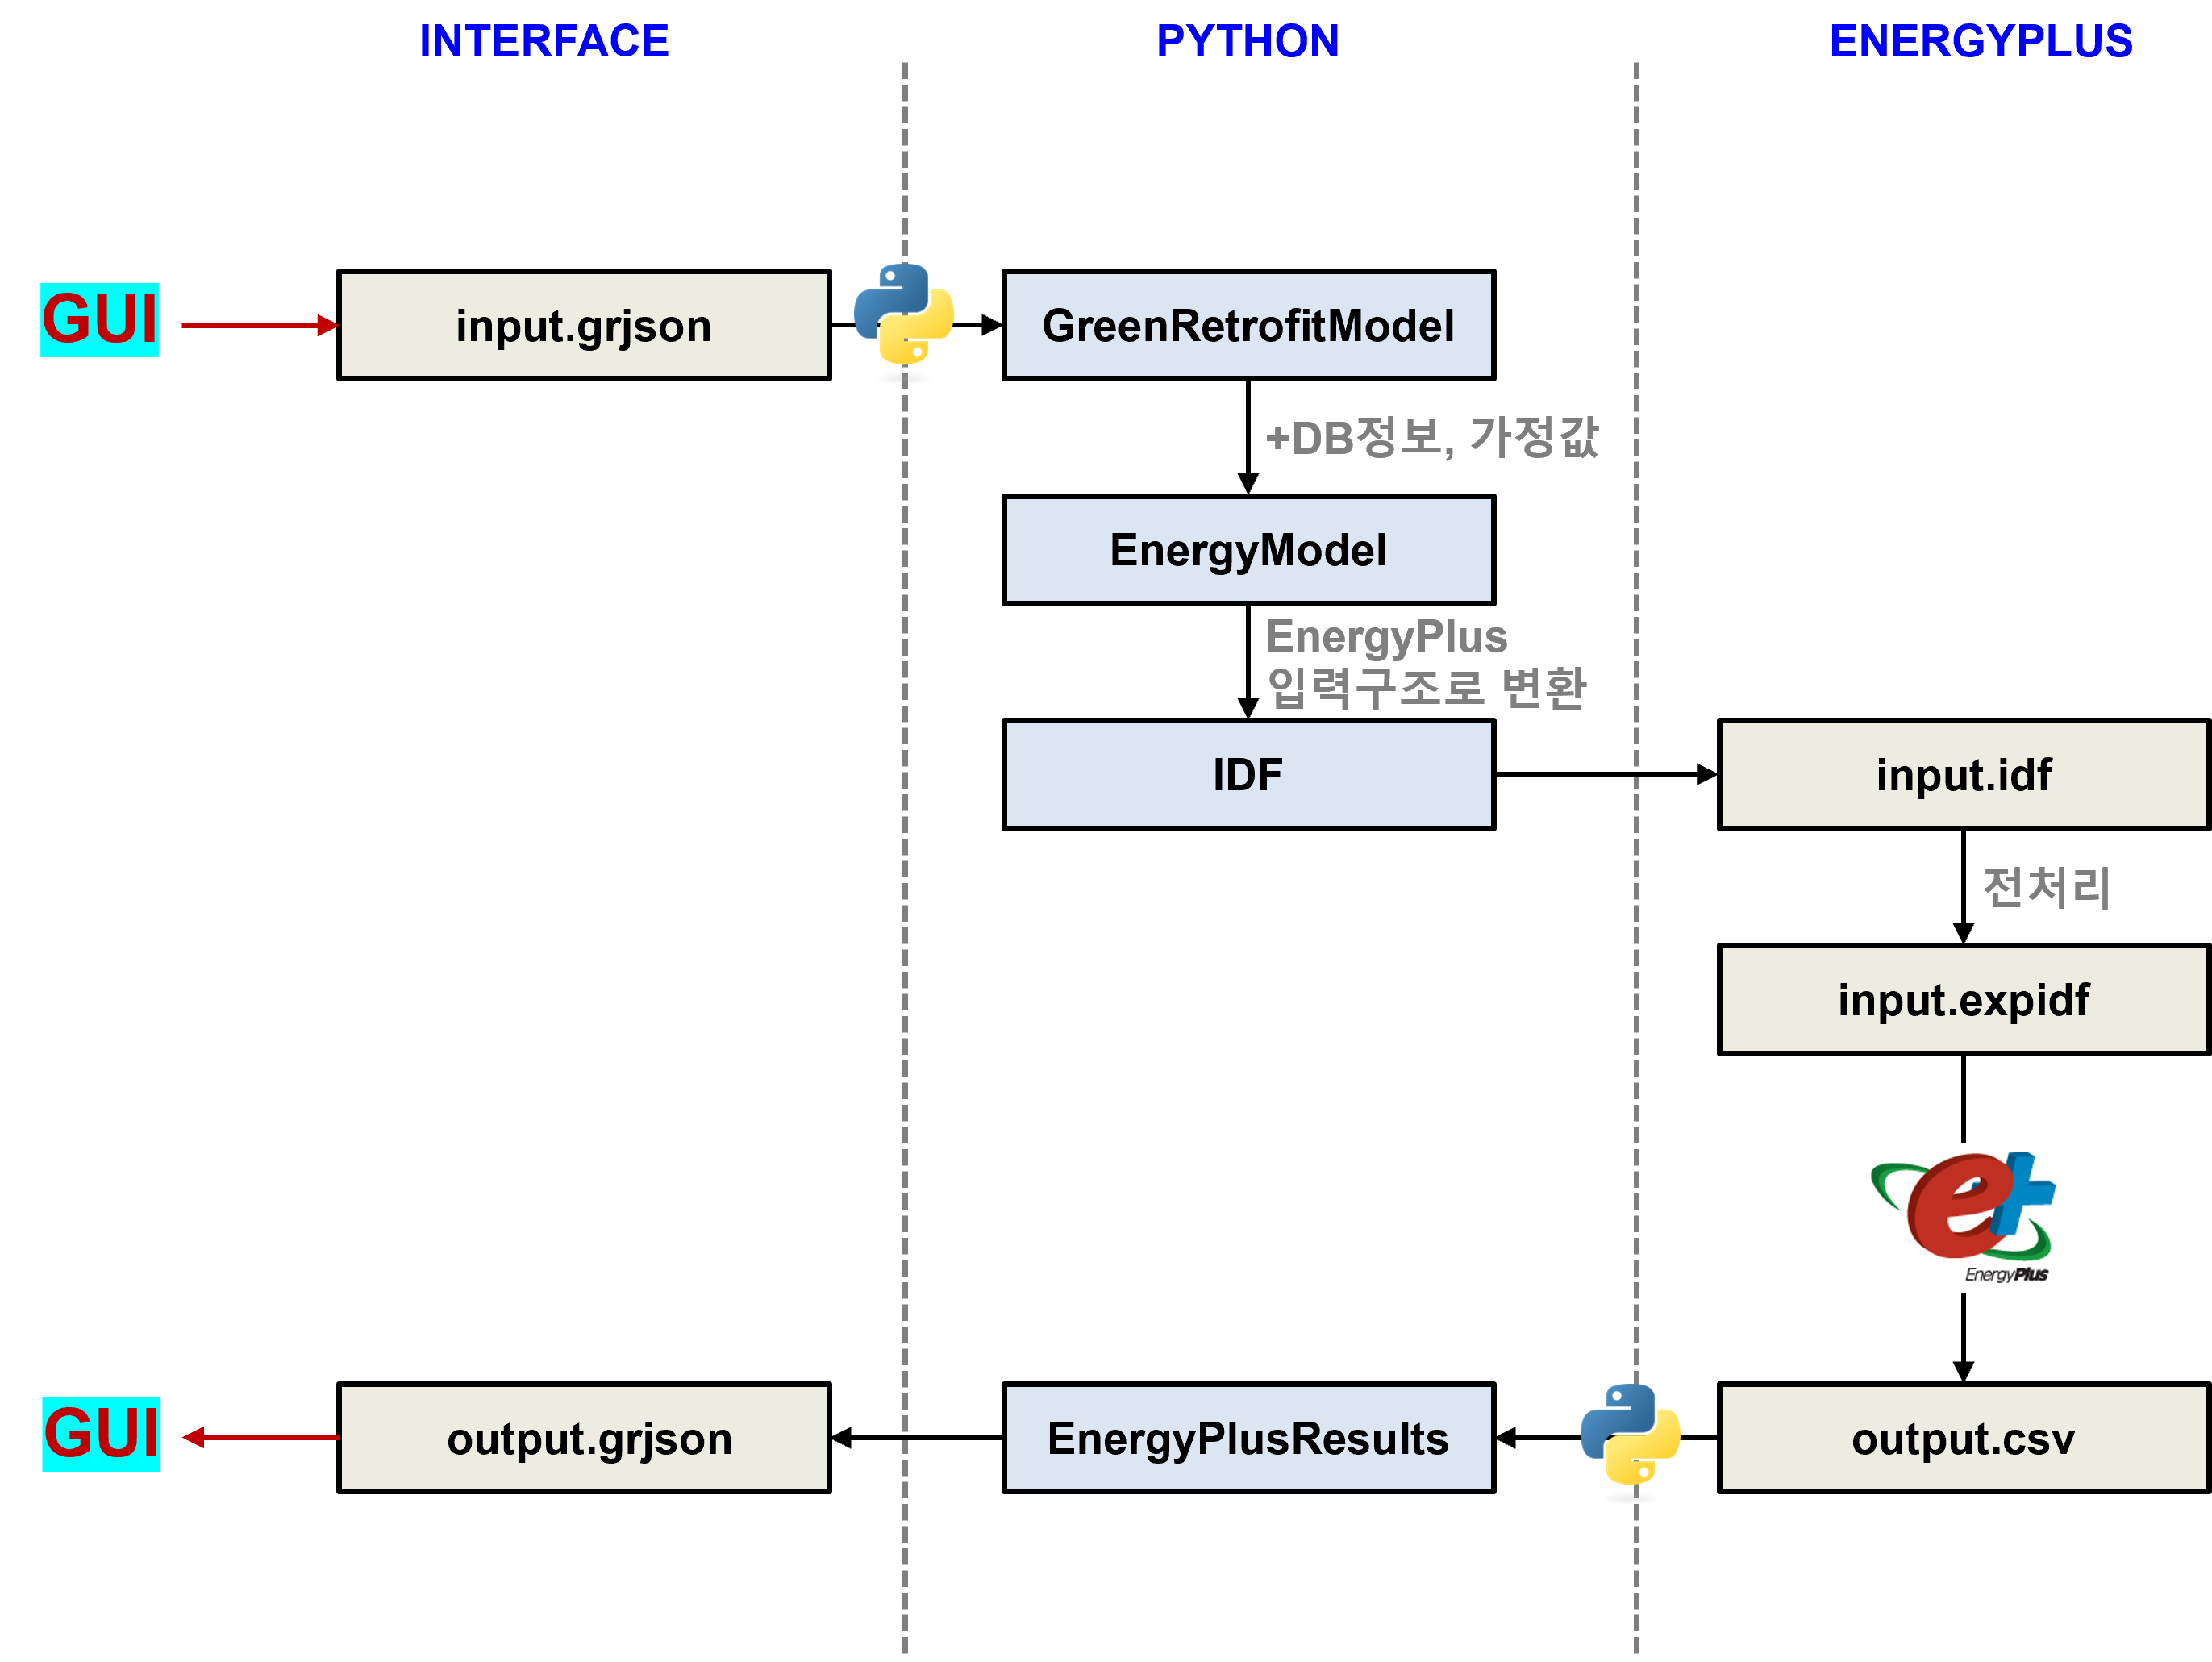
\includegraphics[width=\textwidth]{GRSimulator의 실체.png}
  \caption{\simulator에서 데이터가 전달되는 과정}
  \label{fig:package_function}
\end{defaultfigure}

% chap2.tex
\part{프로그램 구성}
\label{part:ioref}

% ---------------------------------------------------------------------------- %
%                                  NEW SECTION                                 %
% ---------------------------------------------------------------------------- %

\chapter{프로그램 구성 요소}
본 시뮬레이터 엔진은 핵심 python 모듈(\pymodule)\을 중심으로 개발되었다. 이 시뮬레이터는 Python(3.12)\cite{python312}\과 EnergyPlus(24-2-0)\cite{energyplus242}\를 별도 설치 없이 실행할 수 있도록 패키징되어, 사용자가 어떤 환경에서도 단독으로 실행 할 수 있는 독립형 실행 환경을 제공한다(Figure \ref{fig:package_structure}). 개발한 python 모듈(\pymodule)에 대한 자세한 내용은 후속 장에서 설명하며, 사용자는 목적에 맞게 해당 모듈을 충분히 수정 및 가공할 수 있다.

\begin{defaultfigure}
  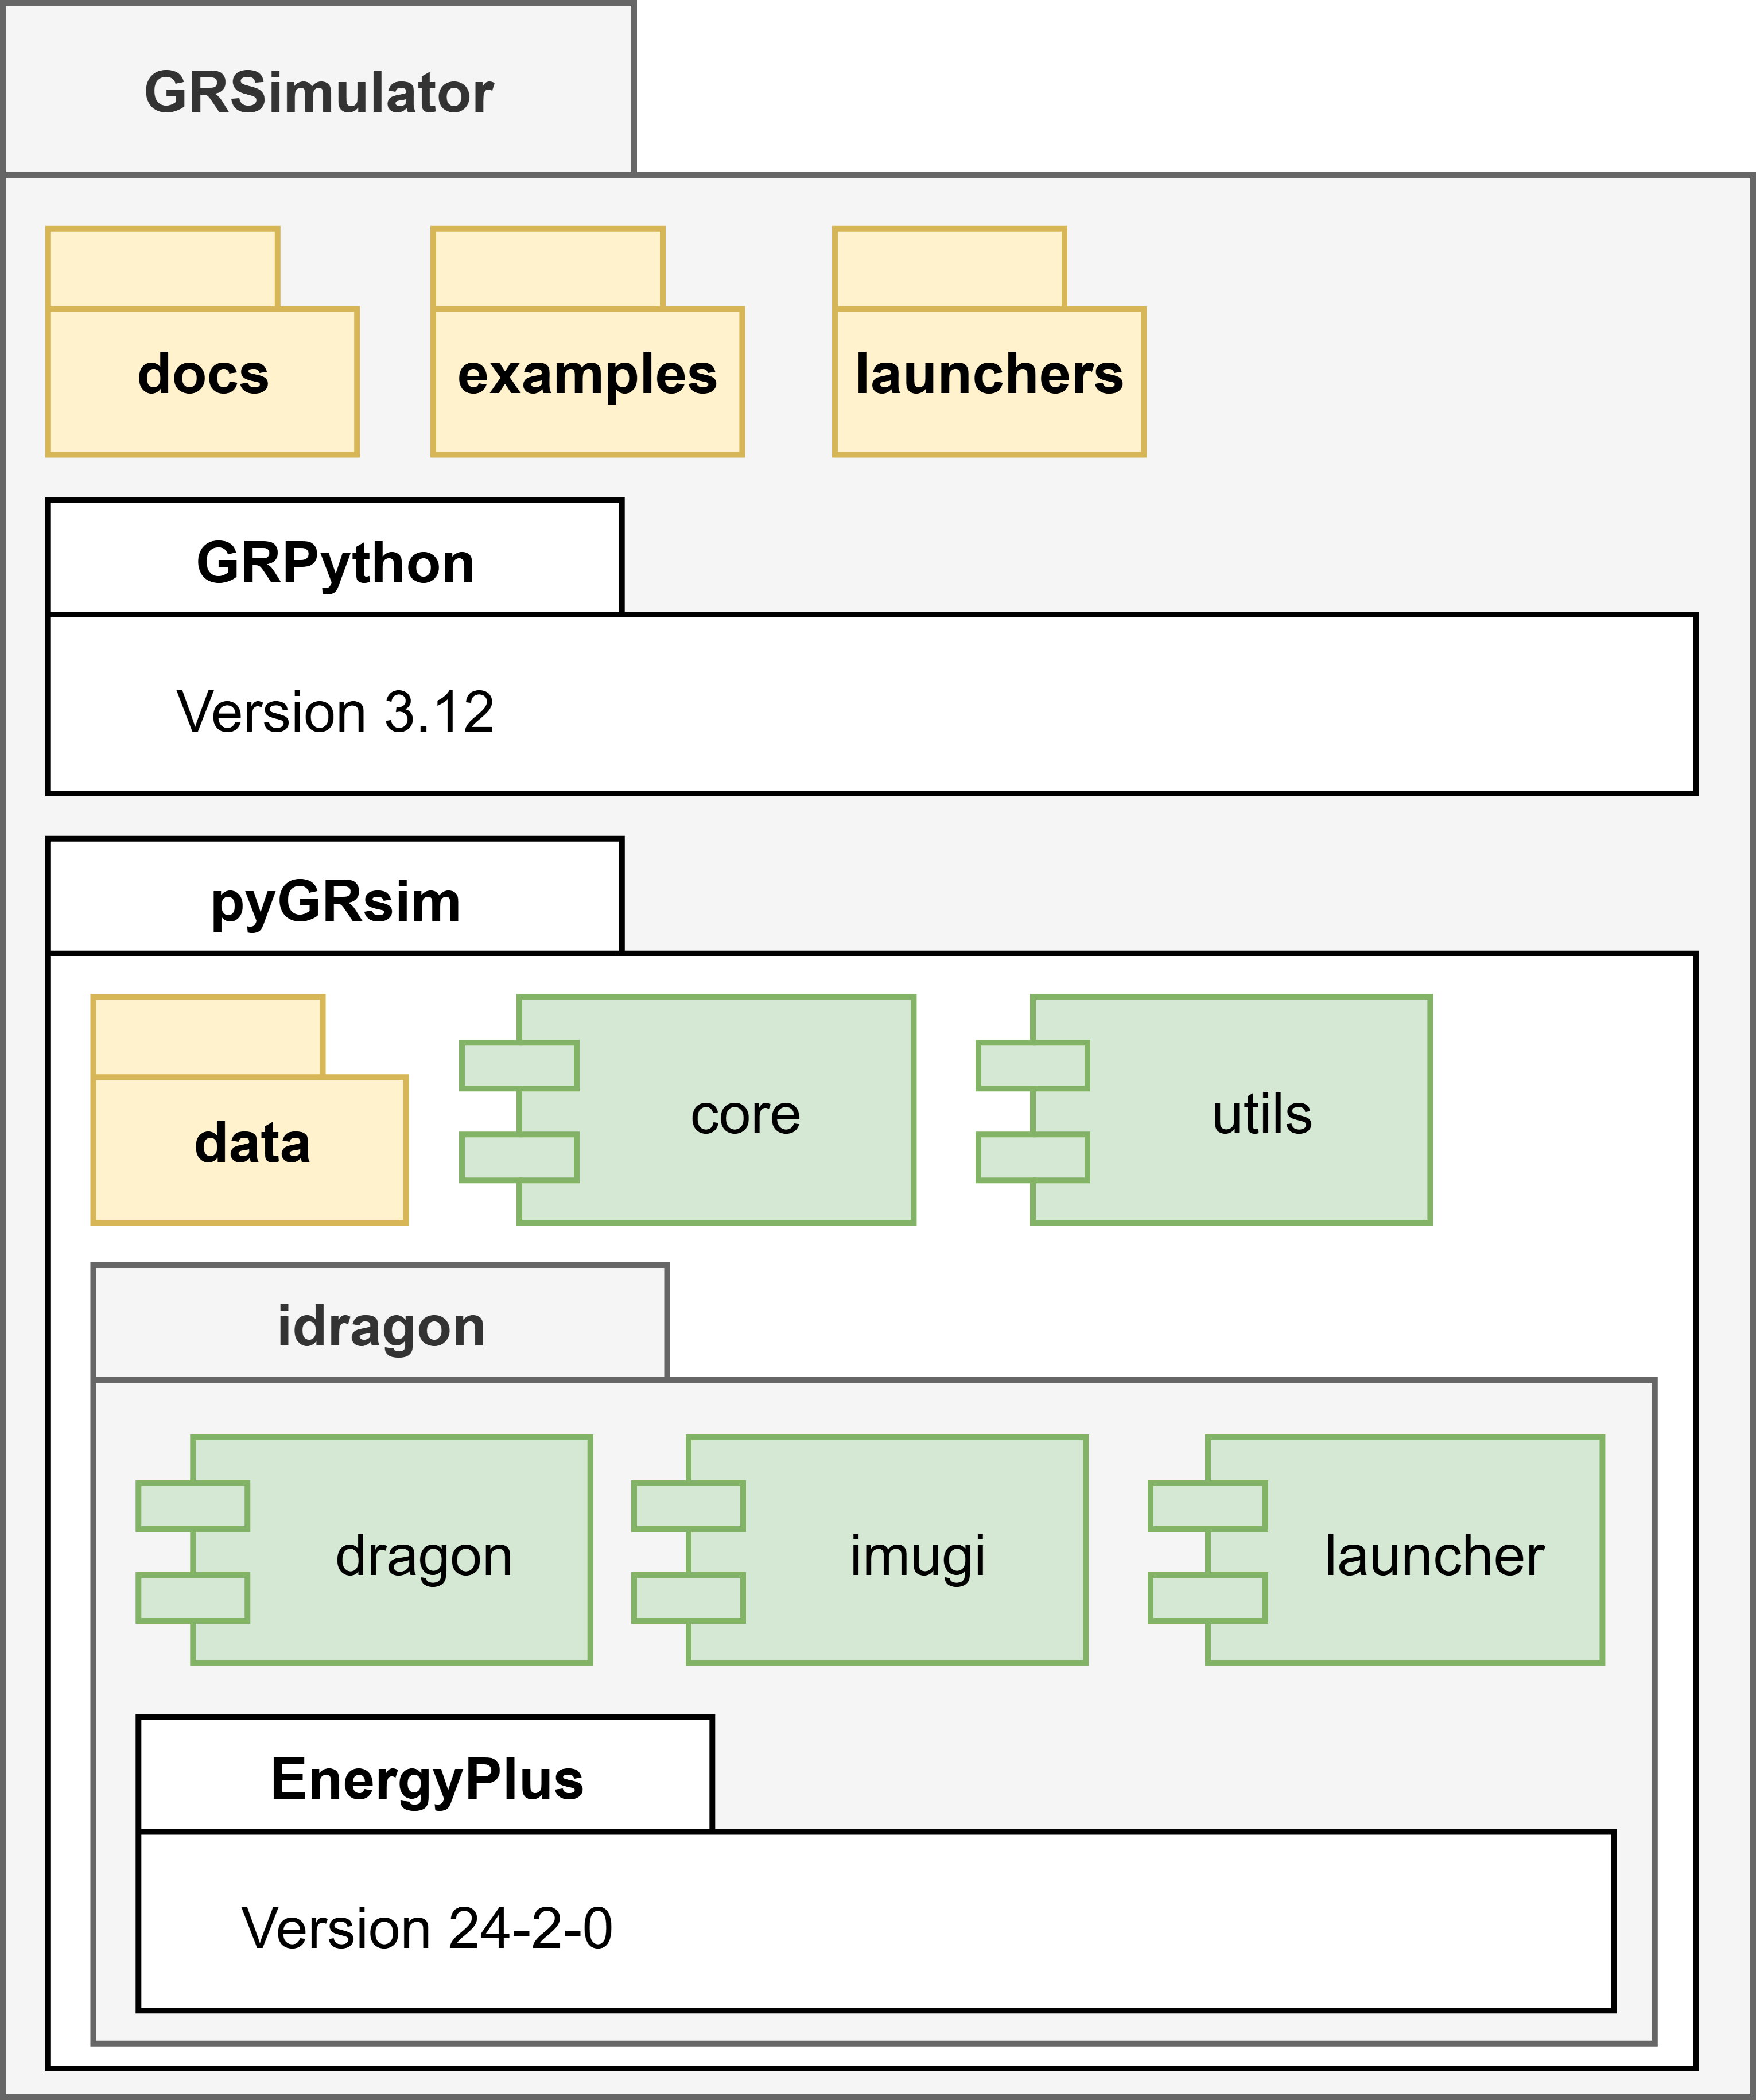
\includegraphics[scale=0.1]{package_structure.png}
  \caption{\simulator\ 프로그램 구조도}
  \label{fig:package_structure}
\end{defaultfigure}

\section{외부 프로그램}

% ---------------------------------------------------------------------------- %
%                                  NEW SECTION                                 %
% ---------------------------------------------------------------------------- %

\subsection{Python 및 그 모듈}
\texttt{Python 3.12}에서 최적화 되었다. \texttt{Python 3.11} 버전과의 호환성도 확인하였으나, 그 이하 버전과의 호환성은 보장하지 않는다.
데이터 처리 및 연산을 위해 \texttt{pandas}와 \texttt{numpy} 라이브러리를 사용한다. 이들 라이브러리의 버전 호환성은 별도로 검증하지 않았으므로, 잠재적인 호환성 문제를 인지하고 있어야 한다.

\subsection{EnergyPlus}
본 시뮬레이터는 \texttt{EnergyPlus 24.2} 버전에 맞추어 개발되었다. EnergyPlus는 하위 및 상위 버전과 호환되지 않으므로, 지원 가능한 버전(24.2)을 설치하도록 주의하여야 한다.\par
참고로, EnergyPlus가 기본 설치 경로(C:/EnergyPlusV24-2-0)에 이미 설치되어 있는 경우, 별도의 패키징 없이도 python 모듈이 해당 경로를 자동으로 찾아 실행할 수 있다. 내 컴퓨터의 EnergyPlus 설치 여부 확인 방법은 아래와 같다.

@TODO (@memo EnergyPlus 파일 찾는법 설명 필요할지?)
를 쓴다. 이건 상하위호환 둘 다 안되니까 설치하려면 정확하게 해야 한다. (사실 될 수도 있는데 굳이 체크 안해봐도 될 듯)\par
참고로 그냥 일반적으로 설치되는 경로인 C:/EnergyPlusV24-2-0에 깔려있으면 이 모듈이랑 같이 묶지 않아도 알아서 찾아서 돌릴 수 있다. EP찾는 순서는 아래와 같다.

\begin{enumerate}
  \item dragon 아래에 있는 EP 폴더
  \item C드라이브에 있는 기본 설치 폴더
  \item 그다음에 내가 그냥 새로 깔기
\end{enumerate}

@TODO
현재(250827) 자동 설치 기능은 지원되지 않으며, 배포 시점에 포함 여부는 미정이다. 따라서, 사용자는 EnergyPlus 24.2를 수동으로 설치하여야 한다.

% ---------------------------------------------------------------------------- %
%                                  NEW SECTION                                 %
% ---------------------------------------------------------------------------- %

\section{예시파일 및 문서}
도 준비되어있다.

설명 문서가 준비되어 있다.
\begin{itemize}
  \item 이 문서랑 별개로 PPT로 만든 사용자 매뉴얼이 제공된다.
  \item 이 문서는 개발자, 연구자용이다.
  \item 개발 과정을 담은 보고서는 어디에 공개되어있으니 별도로 참고 바람.
\end{itemize}

예시파일들도 준비되어있다. 표준입력과 출력을 n개 건물에 대하여 준비하였다.
(이 건물들을 어떻게 정의할 것인지, 건물명을 노출하지 않더라도 그 모델을 노출하는 것이 맞을지 논의가 필요할 듯)

\begin{itemize}
  \item grjson   예시도 준비되어있다.
  \item grexcel  예시도 준비되어있다.
  \item grresult 예시도 준비되어있다.
\end{itemize}


% ---------------------------------------------------------------------------- %
%                                  NEW SECTION                                 %
% ---------------------------------------------------------------------------- %

\section{보조 프로그램들}
도 만들어봤다. @TODO
bat파일로 만든거니까 실행할 때 조심하시고.. 서버 안꺼질 수도 있으니까 조심하시고... \textbackslash taskkill로 백그라운드에서 실행되고 있는 python을 모두 끈 후 실행이 필요. \par
현재 수준으로 GUI 배포는 어렵고, JS로 진행 예정.  (@memo 형곤 이부분 수정)

\subsection{grexcel 검토 launcher}
CHECK\_GREXCEL.bat 파일 실행하면 된다. 그럼 이런 창이 뜬다 (Figure \ref{fig:grjson_checker_capture}).
파일 선택누르고 check 누르면 좀 기다려야 한다. 다 되면 초록색으로 이렇게 뜬다.

\begin{defaultfigure}
  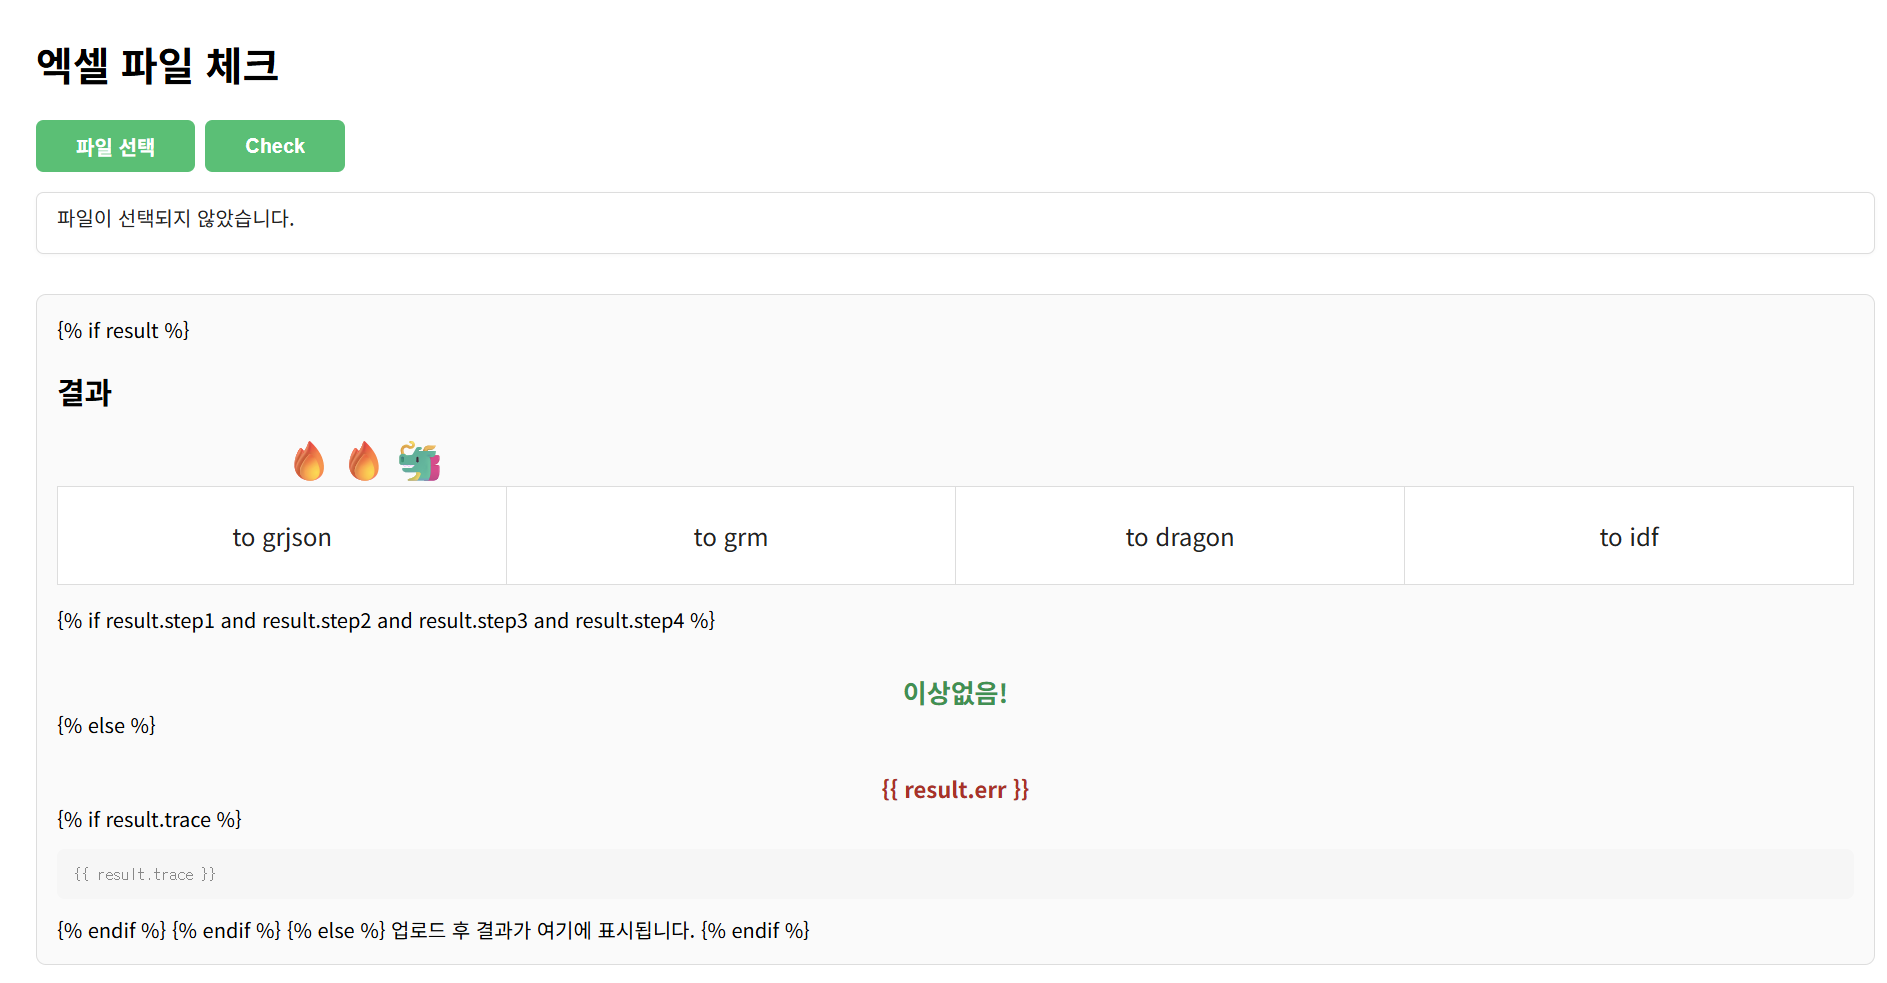
\includegraphics[width=\textwidth]{grexcel checker 캡처.png}
  \caption{grexcel checker 실행하면 나오는 페이지}
  \label{fig:grjson_checker_capture}
\end{defaultfigure}

\subsection{grexcel 및 grjson 실행 launcher}
RUN\_GREXCEL.bat 파일 실행하면 된다. 그럼 이런 창이 뜬다 (Figure \ref{fig:grjson_launcher_capture}).

\begin{defaultfigure}
  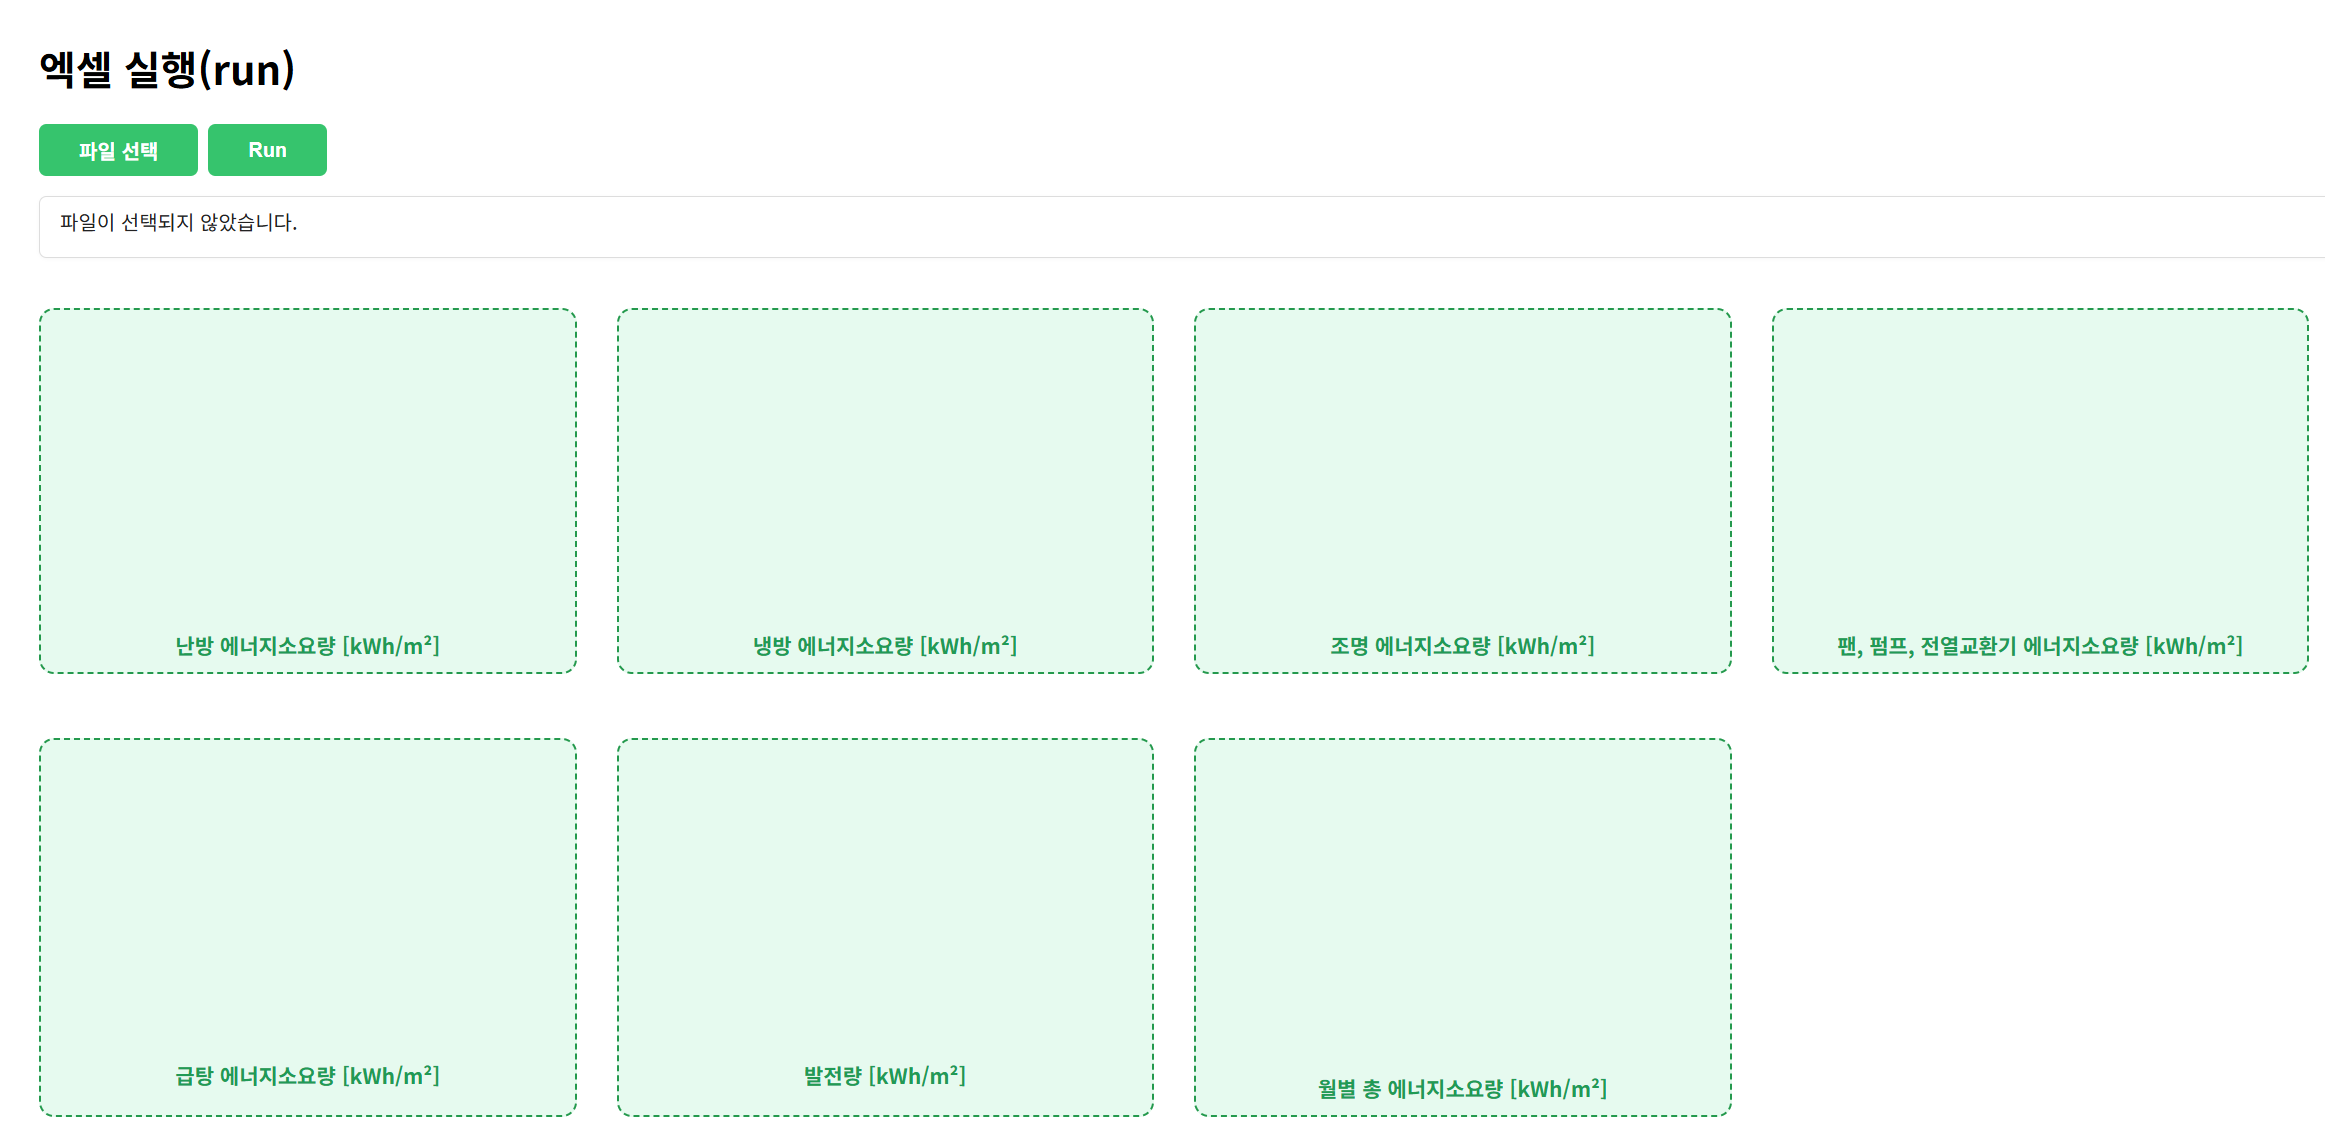
\includegraphics[width=\textwidth]{grexcel launcher 캡처.png}
  \caption{grexcel runner 실행하면 나오는 페이지 (시뮬레이션 전)}
  \label{fig:grjson_launcher_capture}
\end{defaultfigure}

파일 선택하고 run 누르면 좀 기다려야 한다. 다 되면 초록색으로 이렇게 (Figure \ref{fig:grjson_launcher_capture_result}) 뜬다.

\begin{defaultfigure}
  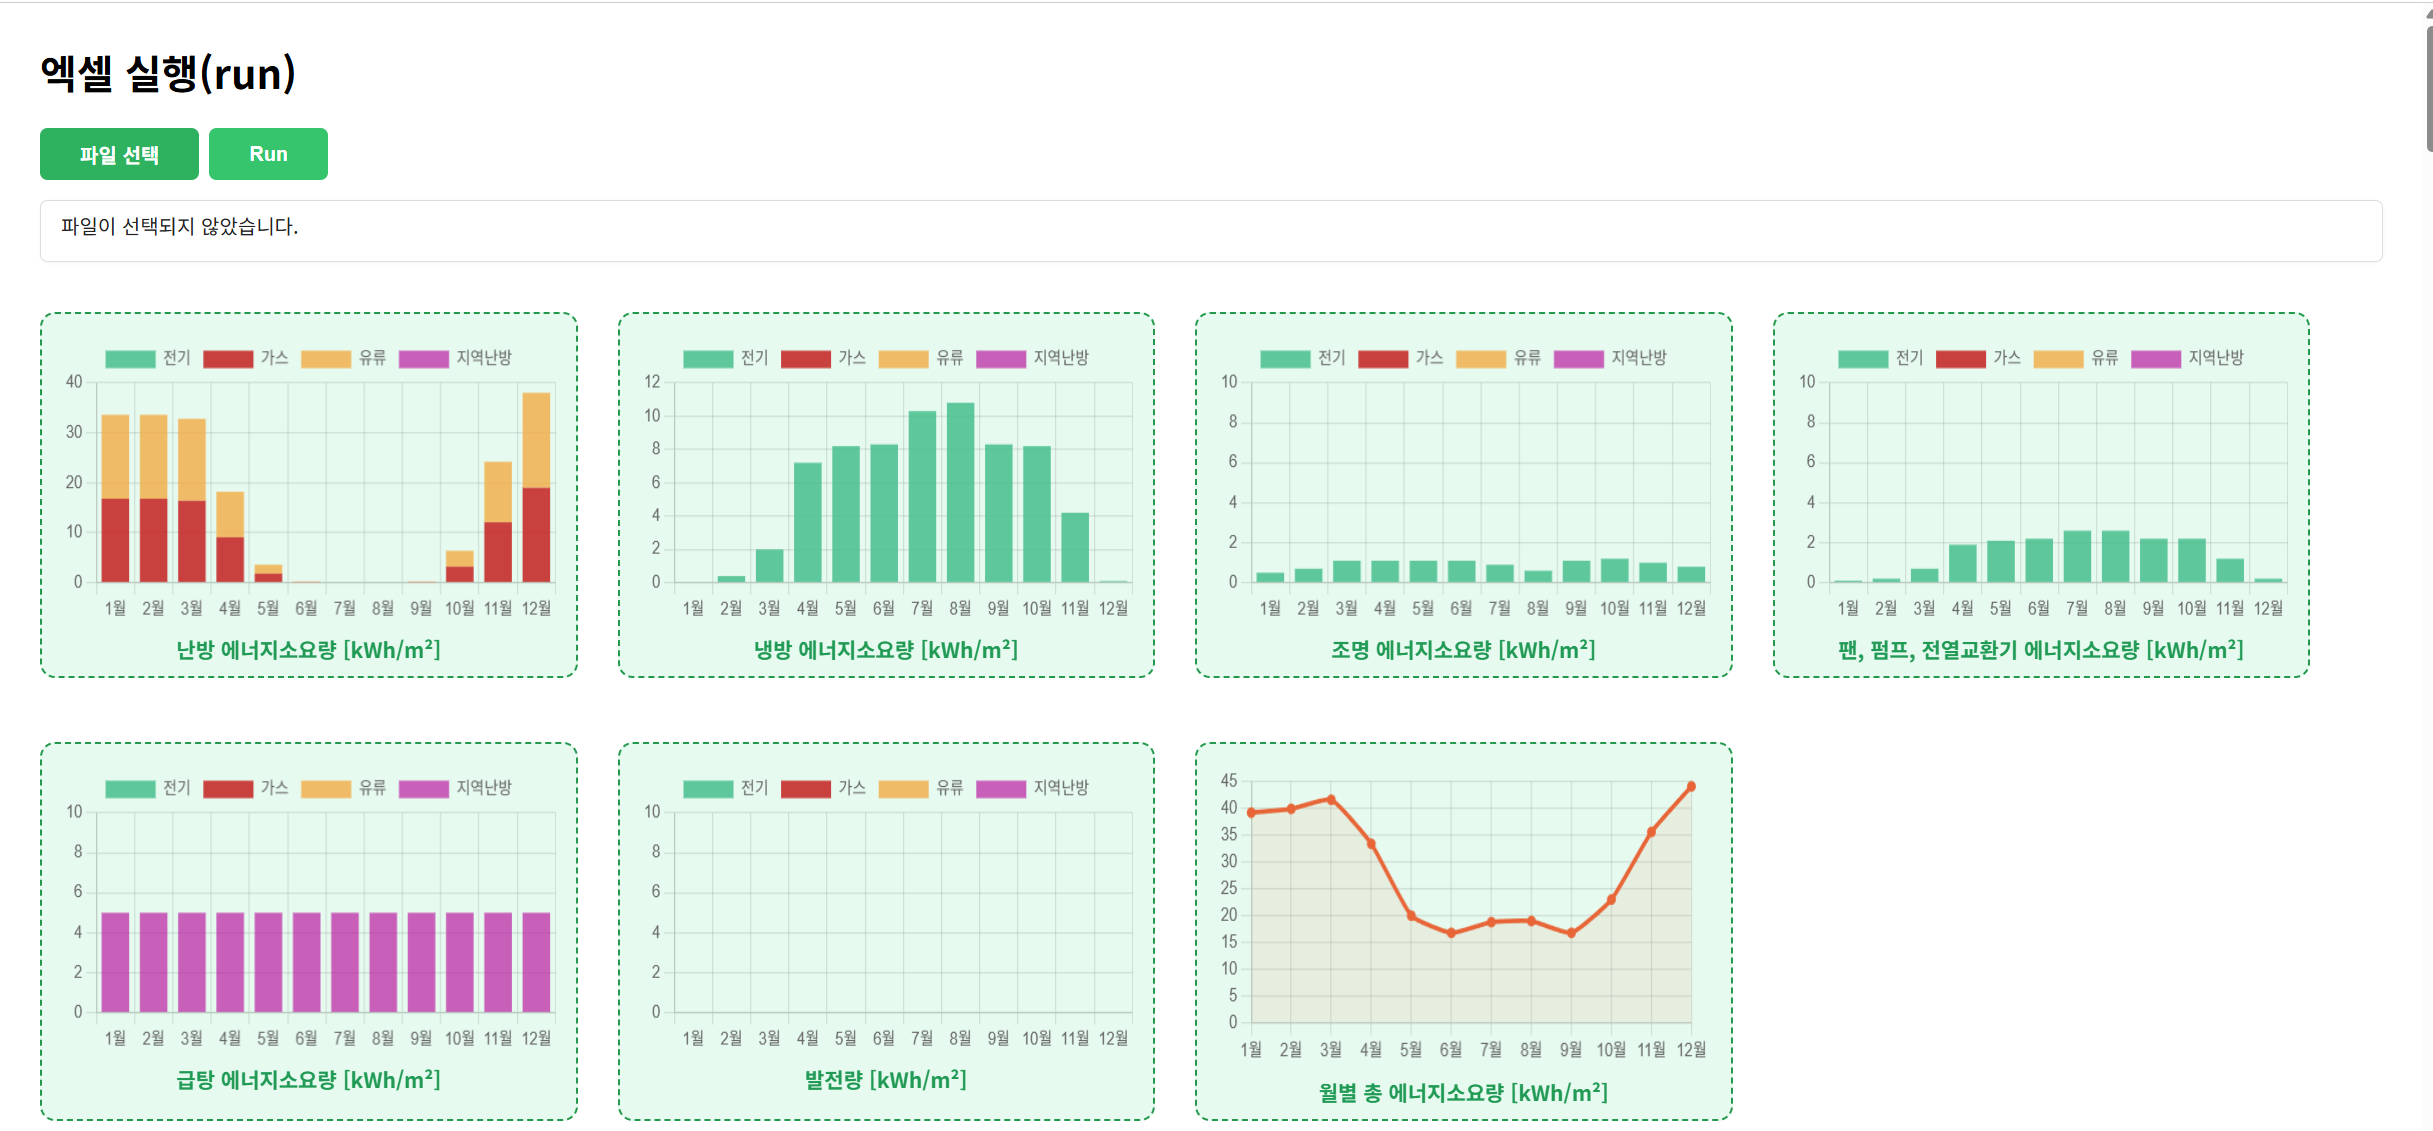
\includegraphics[width=\textwidth]{grexcel launcher 캡처 (결과).png}
  \caption{grexcel runner 실행하면 나오는 페이지 (시뮬레이션 후)}
  \label{fig:grjson_launcher_capture_result}
\end{defaultfigure}


% ---------------------------------------------------------------------------- %
%                                  NEW SECTION                                 %
% ---------------------------------------------------------------------------- %

\section{api}
\subsection{python 모듈의 실행 구조}
python -m 모듈이름 으로 시작하는거다. 우리 모듈도 똑같음 그걸 기대하고 만든것임 \_\_main\_\_.py가 진입점임.

\subsection{api 개발 원칙}
원칙까지는 없을듯.

\subsection{주요 api}

\subsubsection{run: grjson 또는 grexcel 실행}
호출하면 실행하는 것임 인자는 -i 또는 --input, -o 또는 --output 등 있음. 예시는 아래 코드 참고
\begin{tcolorbox}[colback=gray!10, colframe=gray!80, boxrule=0.5pt, left=1em, right=1em]
GRPython/python.exe -m pyGRsim run -i ...path\_to\_input/my\_grjson.grm
\end{tcolorbox}

\subsubsection{DB: DB값 조회}
호출하면 DB 조회하는 것임. DB 이름이랑 key를 보내면 됨. 예시는 아래 코드 참고.

\begin{tcolorbox}[colback=gray!10, colframe=gray!80, boxrule=0.5pt, left=1em, right=1em]
GRPython/python.exe -m pyGRsim run -i ...path\_to\_input/my\_grjson.grm
\end{tcolorbox}

참고로 surface construction이랑 fenestration construction은 \&로 묶은 key를 보내면 법규기준을 return하고 있음. \&로 묶을 수 있는 아이템들은 아래 참고 바람.

% ---------------------------------------------------------------------------- %
%                                  NEW SECTION                                 %
% ---------------------------------------------------------------------------- %
\chapter{입력 및 출력 파일 명세}

\section{\simulator의 데이터 구조}
본 엔진의 입력 데이터는 건물 데이터와,... 이다 (\ref{fig:grjson_structure}).

\begin{defaultfigure}
  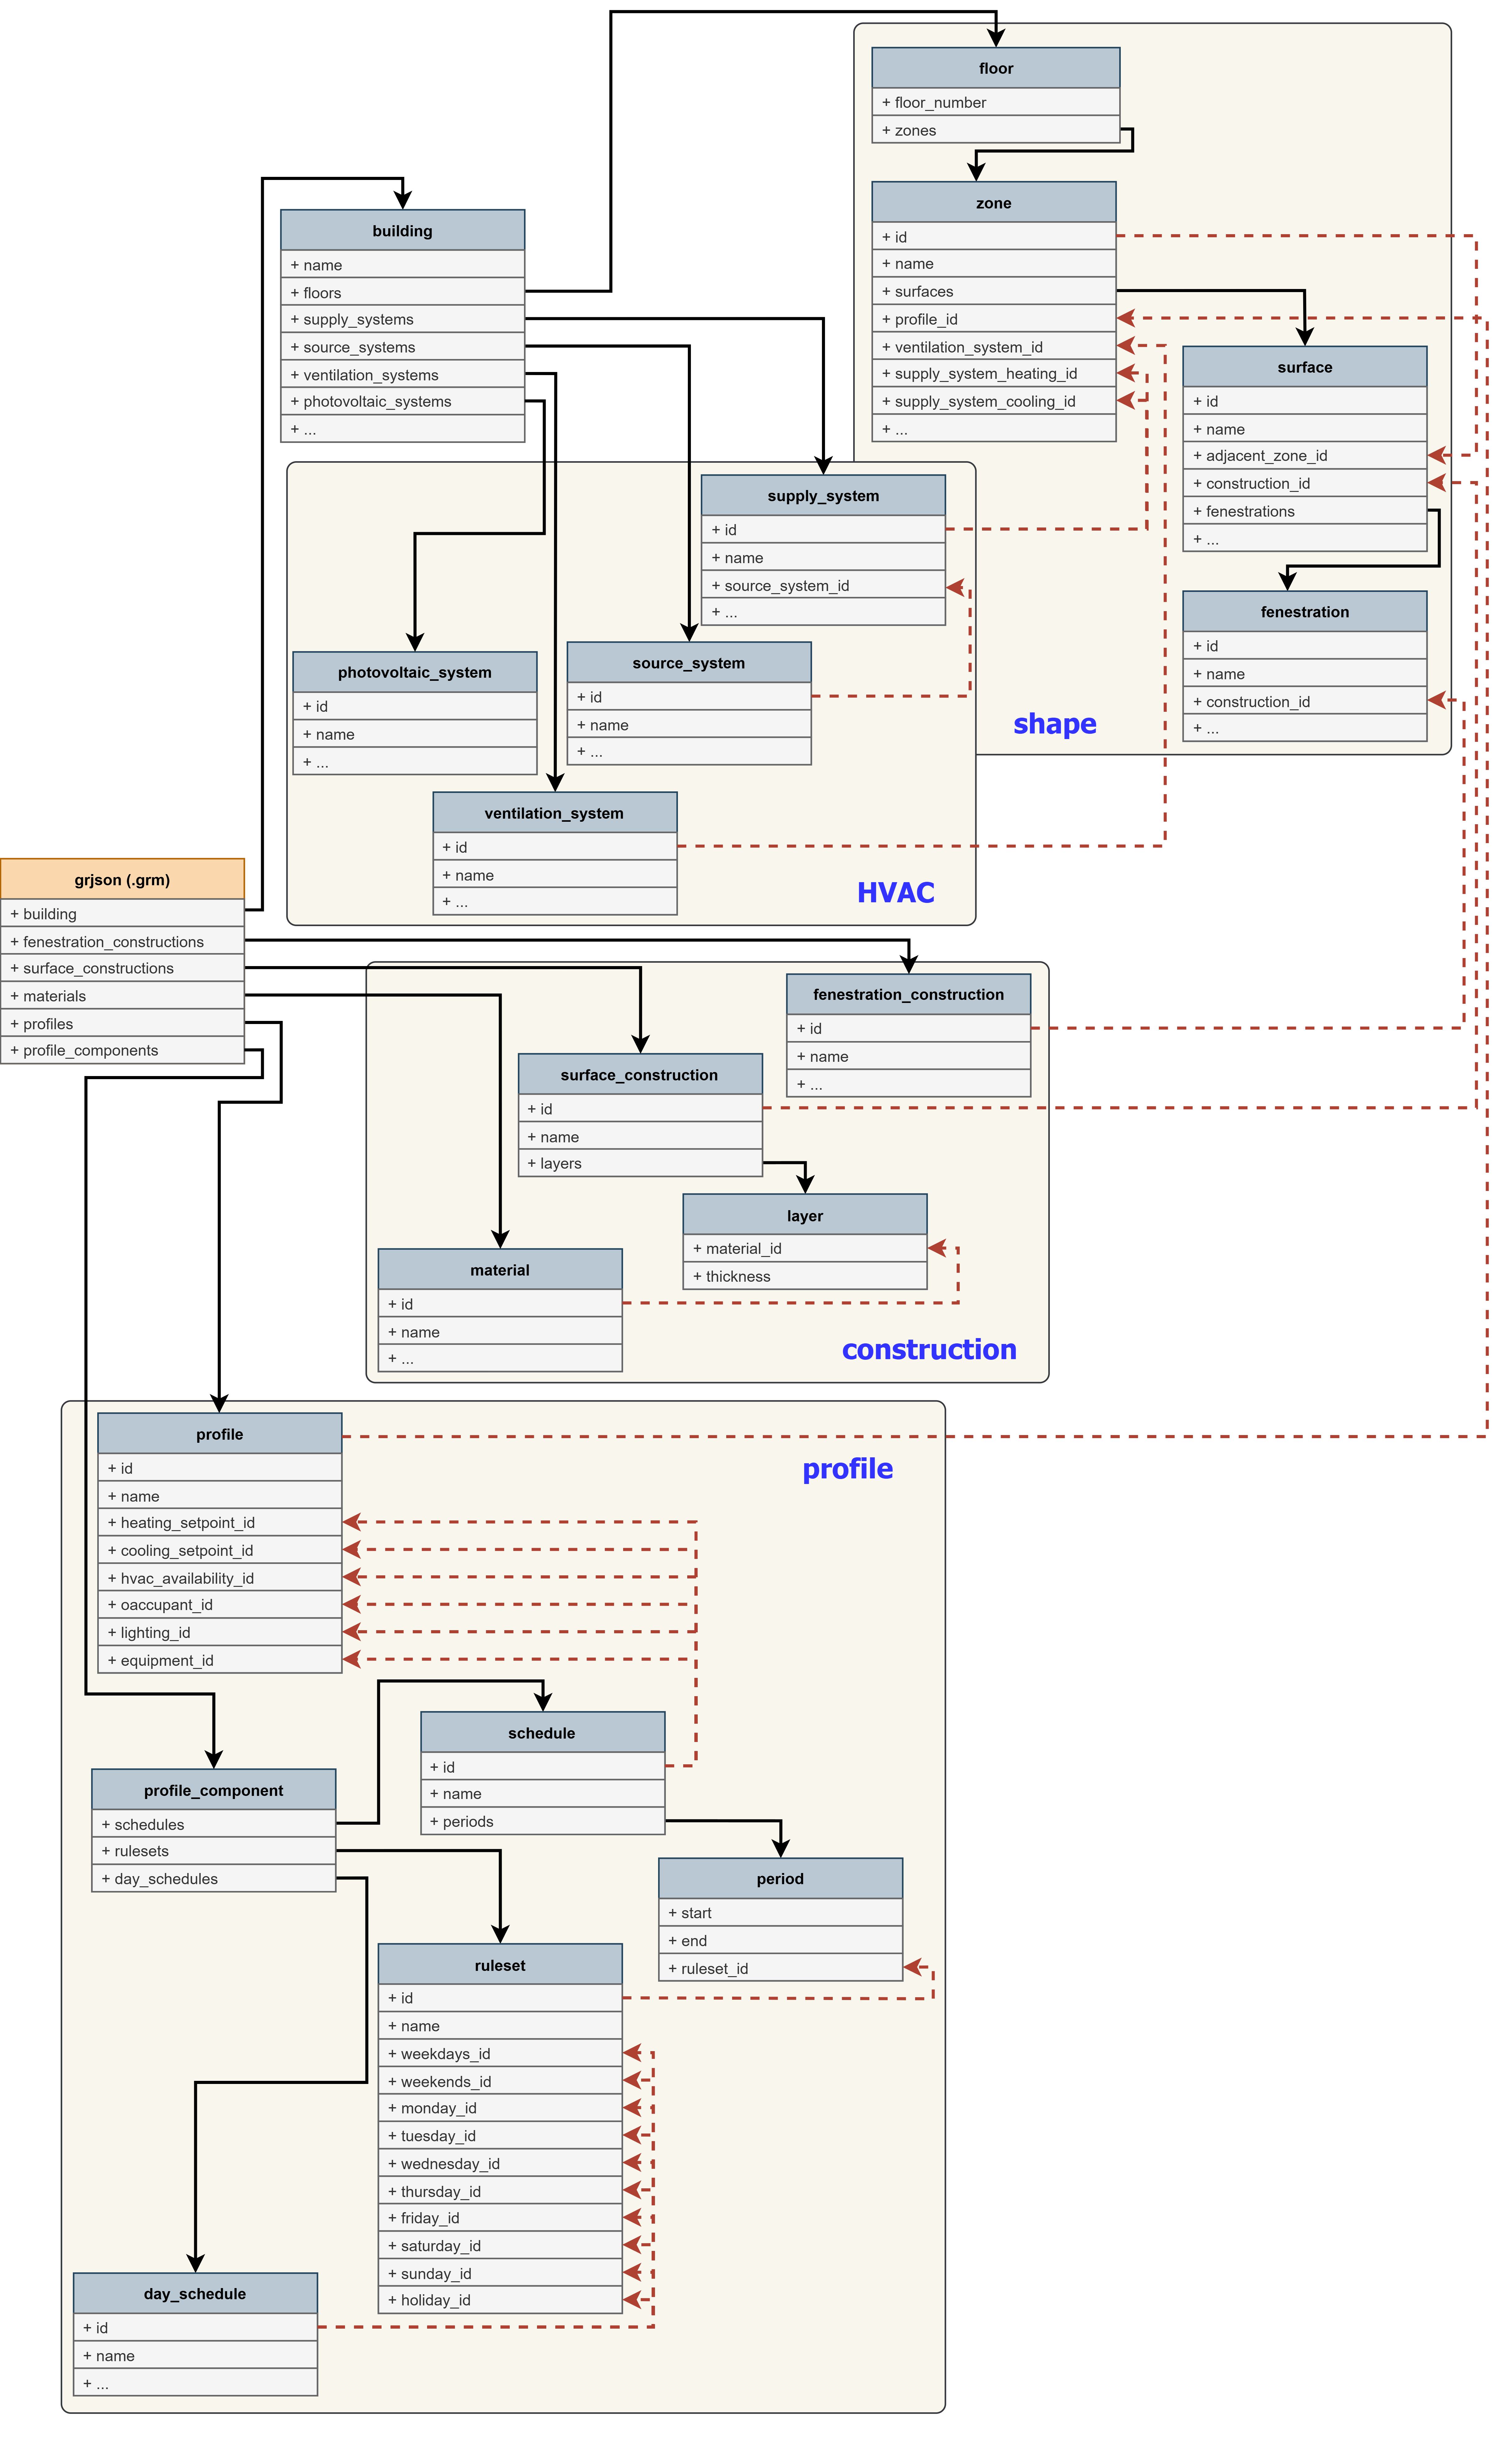
\includegraphics[height=0.99\textheight]{grjson_input_structure_v3.png}
  \caption{\simulator\ 입력변수 체계도}
  \label{fig:grjson_structure}
\end{defaultfigure}

% ---------------------------------------------------------------------------- %
%                                  NEW SECTION                                 %
% ---------------------------------------------------------------------------- %

\section{grjson 구조 (.grm 파일)}

\subsection{규칙}

\subsubsection{변수의 명칭 관련}

\paragraph{사용가능한 문자} 모든 변수의 명칭은 영문 소문자 및 밑줄(\_)로만 구성한다.

\paragraph{복수형과 단수형} 복수 객체 \texttt{array}를 담는 변수의 명칭(예: ``floors") 또는 복수 객체를 담는 하위 분류를 사용하는 변수의 명칭(예: ``profile\_components"), 길는 복수형을 사용하며, 단일 값을 담는 변수의 명칭(예: ``name")은 단수형을 사용한다. 단, 길이가 정해져있거나 각 위치별 의미가 명시적으로 다른 \texttt{array}를 담는 변수의 명칭(예: ``vintage")은 단수형을 사용한다.

\paragraph{축약형의 사용} 모든 변수의 명칭은 축약형을 사용하지 않는 것을 원칙으로 하되, 약어 자체로 통용되는 경우(예: ``cop\_heating")에는 축약형을 사용한다.

\subsubsection{ID 기반 객체 참조 관련} \label{subsubsection:ioref:id_description}
grjson에서 다른 객체의 지칭은 \texttt{ID}값에 기반하여 이루어지며, 모든 객체의 이름(``name")은 사용자 편의를 위한 이름으로 실제 데이터 변환 과정에서 사용되지 않는다.

\paragraph{사용가능한 문자} 모든 ID는 영문 대소문자, 숫자, 하이픈(-), 밑줄(\_)로만 구성되며, 숫자, 하이픈(-) 또는 밑줄(\_)로 시작하지 않는다.

\paragraph{ID의 중복} 동일한 \texttt{ID}는 같은 \texttt{class}의 객체끼리 공유할 수 없다. (모든 \texttt{class}에 대하여 서로 다른 \texttt{ID} 사용을 권장)

\subsubsection{변수의 유효성}

% ------------------------------- 여기서만 쓰는 함수들 ------------------------------- %

% --- 공통 chip (그대로 사용) ---
\newtcbox{\tagchip}[1][]{%
  on line, boxsep=0.6ex, left=0.9ex, right=0.9ex, top=0.2ex, bottom=0.2ex,
  arc=2.2pt, boxrule=0pt, colframe=white,
  colback=black, coltext=white, fontupper=\sffamily\bfseries\footnotesize,
  #1}

% --- 타입 색상 ---
\definecolor{typeString}{RGB}{206,145,120}
\definecolor{typeFloat}{RGB}{181,206,168}
\definecolor{typeInt}{RGB}{78,201,176}
\definecolor{typeEnum}{RGB}{86,156,214}
\definecolor{typeBool}{RGB}{142,206,221}

% --- 요구수준 색상 ---
\definecolor{reqBlueDark}{RGB}{37,99,235}
\definecolor{reqBlueLight}{RGB}{147,197,253}
\definecolor{reqGrayDark}{RGB}{107,114,128}
\definecolor{reqGrayLight}{RGB}{209,213,219}

% --- TypeTag (S/F/I/E) ---
\newcommand{\TypeTag}[1]{%
  \begingroup
  \ifthenelse{\equal{#1}{S}}{\tagchip[colback=typeString,coltext=black]{S}}{%
  \ifthenelse{\equal{#1}{F}}{\tagchip[colback=typeFloat ,coltext=black]{F}}{%
  \ifthenelse{\equal{#1}{I}}{\tagchip[colback=typeInt   ,coltext=white]{I}}{%
  \ifthenelse{\equal{#1}{E}}{\tagchip[colback=typeEnum  ,coltext=white]{E}}{%
  \ifthenelse{\equal{#1}{B}}{\tagchip[colback=typeBool  ,coltext=white]{B}}{%
  \tagchip[colback=gray!60,coltext=black]{#1}}}}}}%
  \endgroup
}

% --- ReqTag (R/CR/O/CO) ---
\newcommand{\ReqTag}[1]{%
  \begingroup
  \ifthenelse{\equal{#1}{R}} {\def\shade{reqBlueDark}\def\fg{white}}{}%
  \ifthenelse{\equal{#1}{CR}}{\def\shade{reqBlueLight}\def\fg{black}}{}%
  \ifthenelse{\equal{#1}{O}} {\def\shade{reqGrayDark}\def\fg{white}}{}%
  \ifthenelse{\equal{#1}{CO}}{\def\shade{reqGrayLight}\def\fg{black}}{}%
  \ifthenelse{\isundefined{\shade}}{\def\shade{gray!60}\def\fg{black}}{}%
  \tagchip[colback=\shade,coltext=\fg]{#1}%
  \endgroup
}

% --- table definition --- 
\newcommand{\jsontableunit}[1]{%
  \ifthenelse{\equal{#1}{}}{-}{$#1$}%
}

\newcommand{\jsontabledash}[1]{%
  \ifthenelse{\equal{#1}{}}{-}{#1}%
}

\newcommand{\jsontablerow}[7]{%
  \nolinkurl{#1} & #2 & #3 &
  \jsontabledash{#4} & \jsontabledash{#5} & \jsontabledash{#6} & \jsontableunit{#7} \\
}

\newcommand{\needtobeexplain}{상세설명 참고}

\newcommand{\jsontable}[2]{
  \begin{table}[htbp]
    \centering
    \caption{grjson 구조에서 \texttt{#1} 클래스의 속성들}
    {\footnotesize
    \begin{tabularx}{\textwidth}{l c c c Y Y c}
      \toprule
      변수명 & 타입 & 필수 & 기본값 & 조건 & 범위/길이/선택지 & 단위 \\
      \midrule
      #2
      \bottomrule
    \end{tabularx}
   } 
  \end{table}
}

모든 변수의 유효성은 필수 및 조건부 사용 여부에 따라 변수(의 속성) 값 존재의 유효성을 검사한 뒤, 타입 및 범위(또는 열거형 상수) 만족 여부를 검사하여 확인할 수 있다.

\paragraph{타입} 모든 변수는 정해진 타입의 변수여야 한다. 모든 변수의 타입은 문자\TypeTag{S}($String$), 실수\TypeTag{F}($Float$), 정수\TypeTag{I}($Integer$), 열거형\TypeTag{E}($Enum$), 불리언\TypeTag{B} 로 구분할 수 있다. 

\paragraph{필수 여부} 입력되지 않을 경우 에러가 발생하는 필수 변수\ReqTag{R}($Required$)와 달리, 비 필수 변수\ReqTag{O}($Optional$)는 미 입력 시 기본값이 사용된다. 단, 입력하지 않았다는 것을 명시적으로 \texttt{null}로 지정해야 하고, 변수 자체를 생락하면 안된다.

\paragraph{조건부 사용 여부} 어떤 변수는 다른 변수(주로 \texttt{type})의 값에 따라 조건부로 사용된다. 이 경우에도 해당 조건에서 필수적으로 요구되는 변수\ReqTag{CR}($Conditional Required$)와 그렇지 않은 변수\ReqTag{CO}($Conditional Optional$)로 구분할 수 있다. 조건에 만족하지 않는 경우, 해당 변수는 json에서 생략될 수 있다.

\paragraph{범위 및 열거형 상수} array면 길이 제약 따짐.
실수\TypeTag{F} 및 정수\TypeTag{I} 타입의 변수는 Python 부동소수점 및 정수 형식에서 표현 가능한 범위 내에서 처리된다.

\subsubsection{기타 규칙}

\paragraph{단위} 모든 변수는 SI 기본단위를 사용한다 (예: $m$, $J$, $W$, $kg$).

\subsection{class별 명세}

\subsubsection{building} \label{subsection:ioref:building}
실재하는 건물에 대한 최상위 정보 체계이다.

\jsontable{building}{
  \jsontablerow{name                 }{\TypeTag{S}}{\ReqTag{R}}{}{}{}{}
  \jsontablerow{north_axis           }{\TypeTag{F}}{\ReqTag{R}}{}{}{[0,360)}{deg(^\circ)}
  \jsontablerow{address              }{\TypeTag{S}}{\ReqTag{R}}{}{}{\needtobeexplain}{}
  \jsontablerow{vintage              }{[ \TypeTag{I} ]}{\ReqTag{R}}{}{}{[3,3]}{}
  \jsontablerow{num_aboveground_floor}{\TypeTag{I}}{\ReqTag{R}}{}{}{[1, $Inf$)}{}
  \jsontablerow{num_underground_floor}{\TypeTag{I}}{\ReqTag{R}}{}{}{[0, $Inf$)}{}
  \jsontablerow{floors               }{[ \hyperref[subsubsection:ioref:floor]{\texttt{floor}} ]}{}{}{}{[1, $Inf$)}{}
  \jsontablerow{supply_systems       }{[ \hyperref[subsubsection:ioref:supplysystem]{\texttt{supply\_system}} ]}{\ReqTag{R}}{}{}{[0, $Inf$)}{}
  \jsontablerow{source_systems       }{[ \hyperref[subsubsection:ioref:sourcesystem]{\texttt{source\_system}} ]}{\ReqTag{R}}{}{}{[0, $Inf$)}{}
  \jsontablerow{ventilation_systems  }{[ \hyperref[subsubsection:ioref:ventilationsystem]{\texttt{ventilation\_system}} ]}{\ReqTag{R}}{}{}{[0, $Inf$)}{}
  \jsontablerow{photovoltaic_systems }{[ \hyperref[subsubsection:ioref:photovoltaicsystem]{\texttt{photovoltaic\_system}} ]}{\ReqTag{R}}{}{}{[0, $Inf$)}{}
}

\paragraph{name} 건물의 이름. 시뮬레이션에 직접 사용되지 않는다.
\paragraph{north\_axis} 건물의 방위각. 도면상에서 나침반이 가리키는 방향 (반시계방향), 또는 건물의 향 관련 입력을 모두 회전시키는 동작 (시계방향) 을 지칭한다 (\cref{fig:ioref:north_axis}).

\begin{defaultfigure}
  
  \begin{subfigure}[b]{0.45\textwidth}
    \centering
    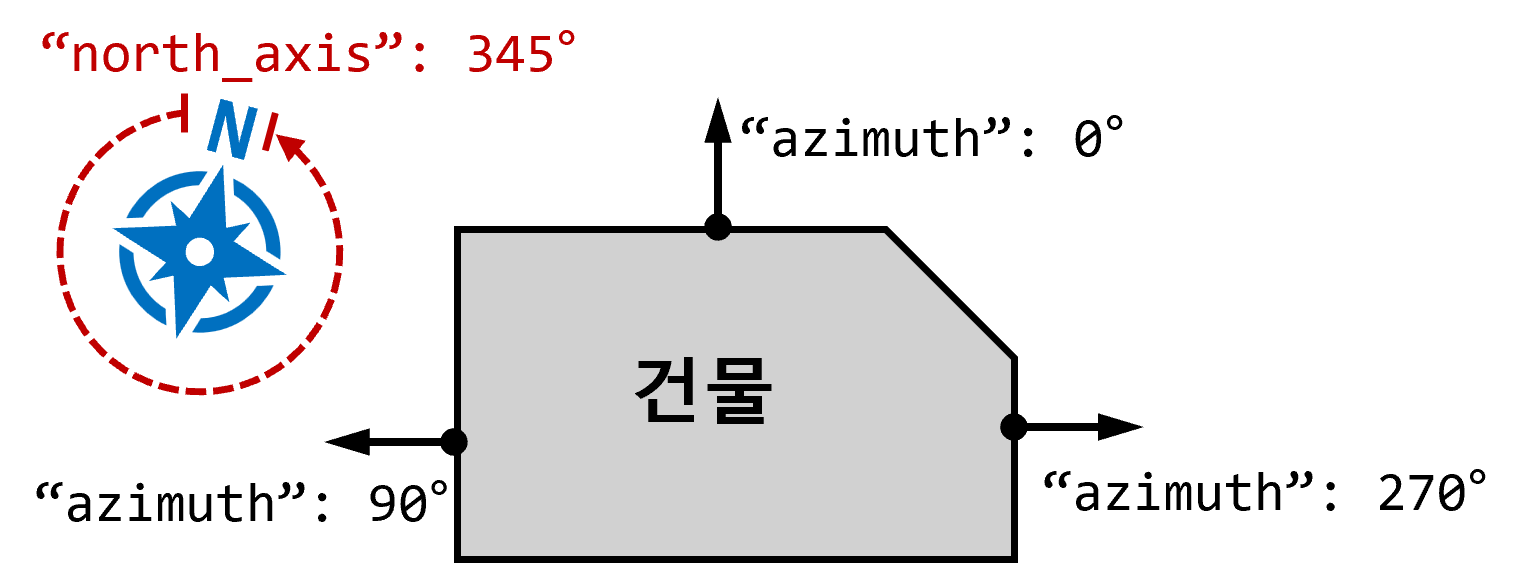
\includegraphics[scale=0.6]{north_axis 설명도식 (도면에서).png}
    \caption{도면에서}
  \end{subfigure}
  \hfill
  \begin{subfigure}[b]{0.45\textwidth}
    \centering
    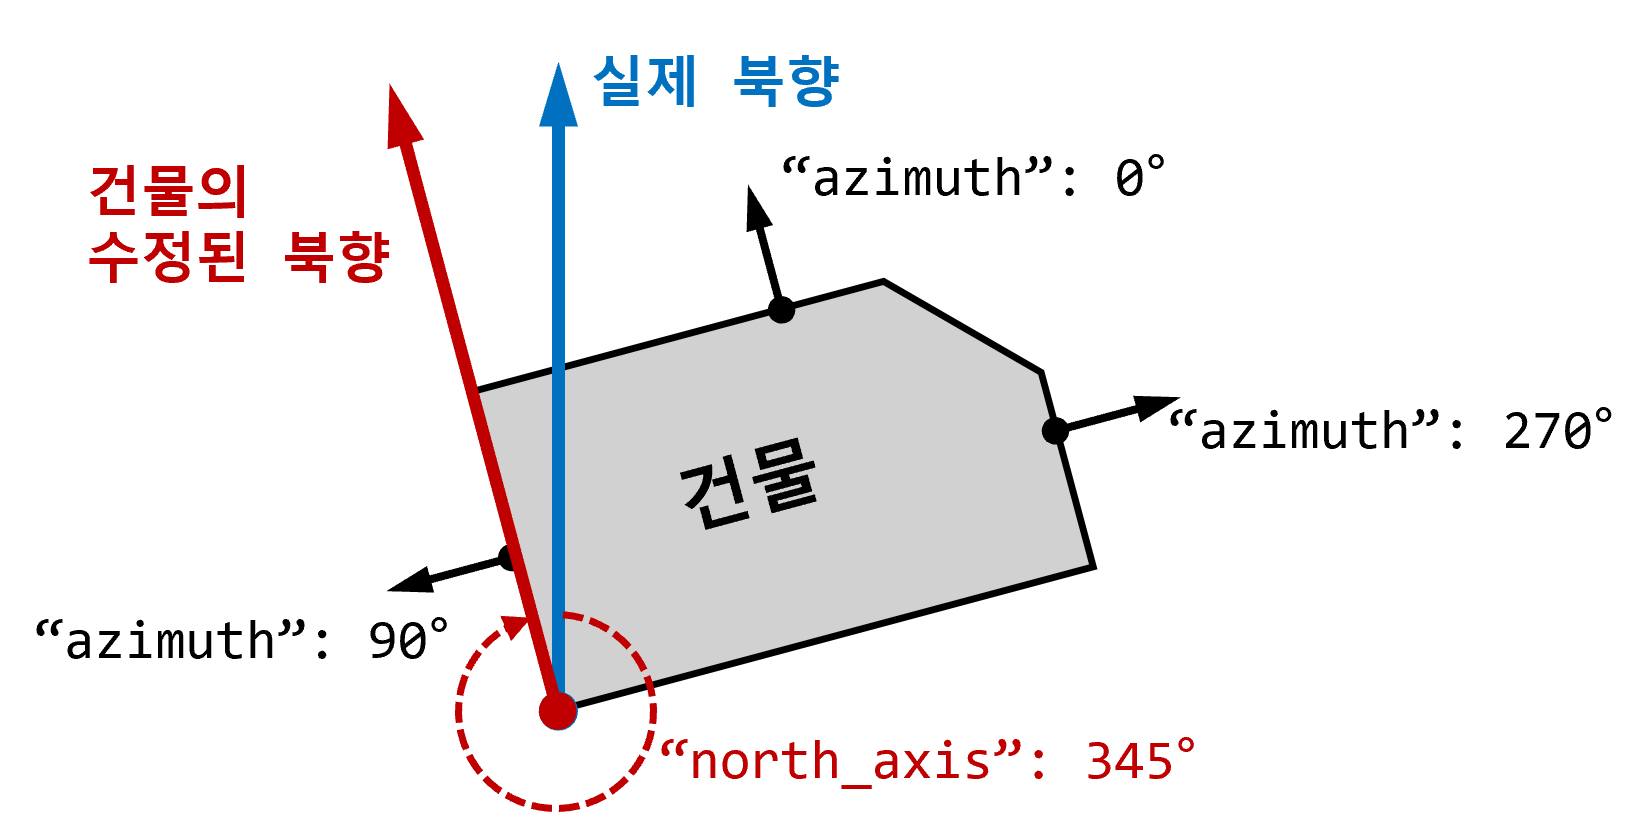
\includegraphics[scale=0.6]{north_axis 설명도식 (지도에서).png}
    \caption{지도에서}
  \end{subfigure}
  
  \caption{north\_axis의 의미와 surface azimuth와의 관계}
  \label{fig:ioref:north_axis}

\end{defaultfigure}

\paragraph{address} 건물의 주소. 식별 가능한 법정 기초행정구역명(세종특별자치시와 제주특별자치도 제주시, 서귀포시를 포함)을 포함하여야 한다. 

\paragraph{vintage} 건물의 허가일자. 연(4자리 정수), 월(2자리 정수), 일(2자리 정수)로 이루어진 array이다.

\paragraph{num\_aboveground\_floor} 건물의 지상 층 수. 시뮬레이션에 직접 사용되지 않는다.

\paragraph{num\_underground\_floor} 건물의 지하 층 수. 시뮬레이션에 직접 사용되지 않는다.

\subsubsection{floor} \label{subsubsection:ioref:floor}
하위 \hyperref[subsubsection:ioref:zone]{\texttt{zone}}들을 층 단위로 구분하기 위한 클래스이다.

\jsontable{floor}{
  \jsontablerow{floor_number}{\TypeTag{I}}{\ReqTag{O}}{0}{}{}{}
  \jsontablerow{zones}{[ \hyperref[subsubsection:ioref:zone]{\texttt{zone}} ]}{\ReqTag{R}}{}{}{[1,$Inf$)}{}
}

\paragraph{floor\_number} 층을 구별하기 위한 식별자. 시뮬레이션에 직접 사용되지 않는다.

\subsubsection{zone} \label{subsubsection:ioref:zone}
건물에서 하나의 실, 또는 같은 열적 특성(유사한 용도, 공통 설비 등)을 공유하는 서로 연결된 여러 실을 모사하는 최소 단위이다.

\jsontable{zone}{
  \jsontablerow{id                      }{\TypeTag{S}}{ \ReqTag{R} }{}{}{}{}
  \jsontablerow{name                    }{\TypeTag{S}}{ \ReqTag{R} }{}{}{}{}
  \jsontablerow{height                  }{\TypeTag{F}}{ \ReqTag{R} }{}{}{(0,$Inf$)}{m}
  \jsontablerow{profile                 }{\TypeTag{S}}{ \ReqTag{R} }{}{}{\needtobeexplain}{}
  \jsontablerow{profile_id              }{\TypeTag{S}}{ \ReqTag{CR}}{}{\texttt{profile} = ``custom''}{\hyperref[subsubsection:ioref:profile]{\texttt{profile}}의 \texttt{id}}{}
  \jsontablerow{light_density           }{\TypeTag{F}}{ \ReqTag{R} }{}{}{[0,$Inf$)}{W/m^{2}}
  \jsontablerow{infiltration            }{\TypeTag{F}}{ \ReqTag{R} }{}{}{[0,$Inf$)}{ACH50}
  \jsontablerow{supply_system_heating_id}{\TypeTag{S}}{ \ReqTag{R} }{}{}{\hyperref[subsubsection:ioref:supplysystem]{\texttt{supply\_system}}의 \texttt{id}}{}
  \jsontablerow{supply_system_cooling_id}{\TypeTag{S}}{ \ReqTag{R} }{}{}{\hyperref[subsubsection:ioref:supplysystem]{\texttt{supply\_system}}의 \texttt{id}}{}
  \jsontablerow{ventilation_system_id   }{\TypeTag{S}}{ \ReqTag{R} }{}{}{\hyperref[subsubsection:ioref:ventilationsystem]{\texttt{ventilation\_system}}의 \texttt{id}}{}
  \jsontablerow{surface                 }{[ \hyperref[subsubsection:ioref:surface]{\texttt{surface}} ]}{ \ReqTag{R} }{}{}{[0, $Inf$)}{}
}

\paragraph{id} 존의 식별자. \ref{subsubsection:ioref:id_description}에 따라 정의된다.

\paragraph{name} 사용자 편의를 위해 제공되는 존 구별 식별자. 중복, 사용가능한 문자에 제한이 없으며, 시뮬레이션에 직접 사용되지 않는다.

\paragraph{height} 존의 높이. 실의 부피 계산에 이용된다.

\paragraph{profile} 존의 용도프로필. 기본으로 제공되는 항목, 또는 ``custom'' 중에서 입력 가능하다. 

\paragraph{profile\_id} 존에 적용된 custom 용도프로필의 ID. 

\paragraph{light\_density} 조명 밀도.

\paragraph{supply\_system\_heating\_id} 난방공급시스템의 ID. 

\paragraph{supply\_system\_cooling\_id} 냉방공급시스템의 ID.

\paragraph{ventilation\_system\_id} 환기시스템의 ID.

\paragraph{surface} 소속면. 해당 \texttt{zone}을 인접존으로 하는 \texttt{surface}를 포함하여, 1개 이상의 천장(\texttt{type} = ``ceiling''), 1개 이상의 바닥(\texttt{type} = ``floor'') 및 1개 이상의 벽체(\texttt{type} = ``wall'')를 필요로 한다. 즉, 인접존이 없을 경우, 3 이상의 길이를 가지는 list가 필요하다.

\subsubsection{surface} \label{subsubsection:ioref:surface}
존과 존, 외부 (외기 또는 지면), 또는 단열선 사이의 면(벽체)이다.

\jsontable{surface}{
  \jsontablerow{id                  }{\TypeTag{S}}{\ReqTag{R} }{}{}{}{}
  \jsontablerow{name                }{\TypeTag{S}}{\ReqTag{R} }{}{}{}{}
  \jsontablerow{type                }{\TypeTag{E}}{\ReqTag{R} }{}{}{\shortstack[c]{floor \\ wall \\ ceiling}}{}
  \jsontablerow{boundary_condition  }{\TypeTag{E}}{\ReqTag{R} }{}{}{\shortstack[c]{outdoors \\zone \\ ground \\ adiabatic}}{}
  \jsontablerow{area                }{\TypeTag{F}}{\ReqTag{R} }{}{}{(0,$Inf$)}{m^2}
  \jsontablerow{azimuth             }{\TypeTag{F}}{\ReqTag{CR} }{}{\texttt{type} = ``wall'' \newline AND \newline \texttt{boundary\_condition} = ``outdoors''}{[0,360)}{deg(^\circ)}
  \jsontablerow{adjacent_zone_id    }{\TypeTag{S}}{\ReqTag{CR}}{}{\texttt{boundary\_condition} = ``zone''}{\hyperref[subsubsection:ioref:zone]{\texttt{zone}}의 \texttt{id}}{}
  \jsontablerow{construction_id     }{\TypeTag{S}}{\ReqTag{R}}{}{}{\hyperref[subsubsection:ioref:construction]{\texttt{construction}}의 \texttt{id} \newline ``open'' \newline ``unknown''}{}
  \jsontablerow{coolroof_reflectance}{\TypeTag{F}}{\ReqTag{CO}}{}{\texttt{type} = ``ceiling'' \newline AND \newline \texttt{boundary\_condition} = ``outdoors''}{(0,1]}{1}
  \jsontablerow{fenestrations       }{[ \hyperref[subsubsection:ioref:fenestration]{\texttt{fenestration}} ]}{\ReqTag{R}}{}{}{[0, $Inf$)}{}
}

\paragraph{id} 면의 식별자. \ref{subsubsection:ioref:id_description}에 따라 정의된다.

\paragraph{name} 사용자 편의를 위해 제공되는 면 구별 식별자. 중복, 사용가능한 문자에 제한이 없으며, 시뮬레이션에 직접 사용되지 않는다.

\paragraph{type} 면의 유형. 천장(``ceiling''), 바닥(``floor''), 벽체(``wall'')로 구분된다. 유형이 바닥(``floor'')인 면의 면적은 해당 \texttt{zone}의 면적에 포함되며, 유형이 천장(``ceiling'')인 면은 경계조건이 외기(``outdoors'')인 경우 쿨루프 적용이 가능하다.

\paragraph{boundary\_condition} 면의 경계조건. 일사와 바람의 영향을 받고 외기와 열교환을 하는 외기(``outdoors''), 다른 \texttt{zone}과 열교환을 하는 존(``zone''), 지면과 열교환을 하는 지면(``ground''), 어떠한 열교환도 하지 않고 축열의 역할만 담당하는 단열(``adiabatic'')로 구분된다 (Figure \ref{fig:surface_bo_description}).

\begin{defaultfigure}
  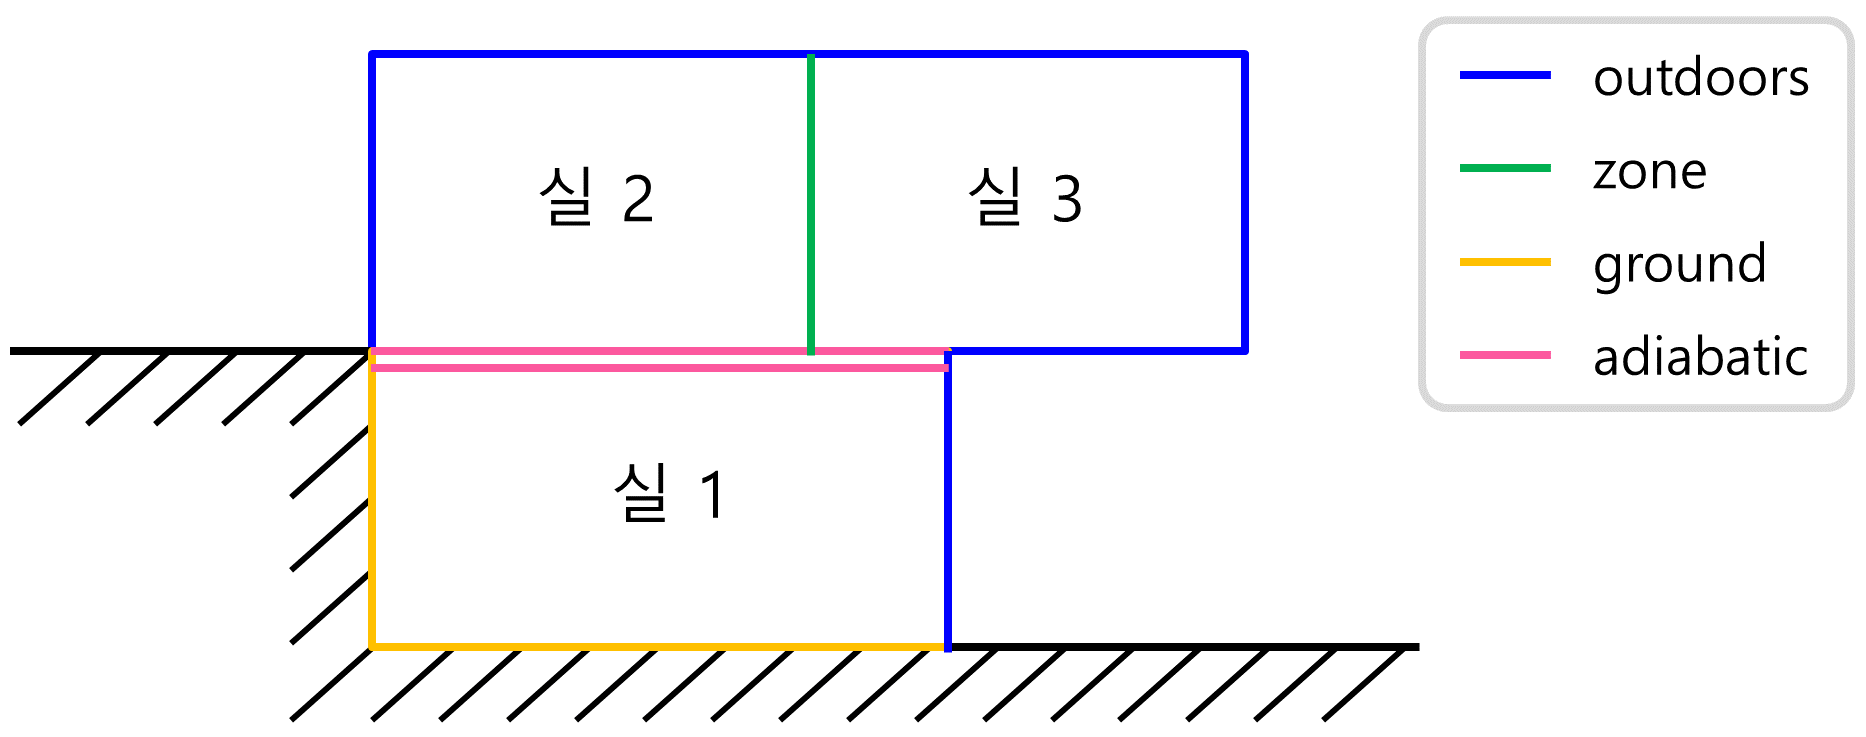
\includegraphics[width=0.8\textwidth]{면 경계조건 예시.png}
  \caption{면의 경계조건 예시}
  \label{fig:surface_bo_description}
\end{defaultfigure}

\paragraph{area} 면적. 해당 면에 개구부(예:창, 문 등)가 존재하는 경우, 이들의 면적을 포함한 전체 면적을 의미한다.

\paragraph{azimuth} 면의 방위각. 기준은 북향을 0$^\circ$로 하며, 반시계 방향으로 증가한다. 예를들어, 서향은 90$^\circ$, 남향은 180$^\circ$, 동쪽은 270$^\circ$로 정의한다.

\paragraph{adjacent\_zone\_id} 인접존 ID. 면의 경계조건을 ``zone''으로 설정한 경우에만 입력한다.

\paragraph{construction\_id} 구조체 ID. 

\paragraph{coolroof\_reflectance} 지붕면의 태양 반사율. 쿨루프(Cool Roof)시공이 적용된 경우에만 입력한다.

\subsubsection{fenestration} \label{subsubsection:ioref:fenestration}
개구부. 벽체의 열린 부분을 의미하며, 창, 문(유리문, 방화문 등) 등 외기와의 접촉 또는 채광·환기를 목적으로 설치된 요소를 포함한다.

\jsontable{fenestration}{
  \jsontablerow{id             }{\TypeTag{S}}{\ReqTag{R}}{}{}{}{}
  \jsontablerow{name           }{\TypeTag{S}}{\ReqTag{R}}{}{}{}{}
  \jsontablerow{type           }{\TypeTag{E}}{\ReqTag{R}}{}{}{\shortstack[c]{window \\ door \\ glassdoor}}{}
  \jsontablerow{area           }{\TypeTag{F}}{\ReqTag{R}}{}{}{(0,$Inf$)}{m^2}
  \jsontablerow{construction_id}{\TypeTag{S}}{\ReqTag{R}}{}{}{\hyperref[subsubsection:ioref:fenestrationconstruction]{\texttt{fenewtration\_construction}}의 \texttt{id}}{}
  \jsontablerow{blind          }{\TypeTag{E}}{\ReqTag{O}}{\texttt{null}}{}{\shortstack[c]{ venetian \\ shade}}{}
}

\paragraph{id} 개구부의 식별자. \ref{subsubsection:ioref:id_description}에 따라 정의된다.

\paragraph{name} 사용자 편의를 위해 제공되는 개구부 구별 식별자. 중복, 사용가능한 문자에 제한이 없으며, 시뮬레이션에 직접 사용되지 않는다.

\paragraph{type} 개구부의 유형. 유리창(``window''), 유리문(``glassdoor''), 또는 유리가 아닌 일반 문(``door'', 예: 방화문, 나무문 등)으로 구분된다.

\paragraph{area} 개구부의 면적. 해당 개구부가 속한 면의 면적보다 작아야 한다.

\paragraph{construction\_id} 개구부의 구조체. \texttt{type}이 ``window'' 또는 ``glassdoor''인 경우, \texttt{is\_transparent} 속성이 \texttt{True}인 구조체여야 한다. 반대로, \texttt{type}이 ``door''인 경우, \texttt{is\_transparent} 속성이 \texttt{False}인 구조체여야 한다

\paragraph{blind} 블라인드의 종류. 값이 \texttt{null}이면 블라인드가 없는 것을 의미한다.

\subsubsection{supply\_system} \label{subsubsection:ioref:supplysystem}
각 존에 존재하는 말단 공급설비이다. 

\jsontable{supply\_system}{
  \jsontablerow{id              }{\TypeTag{S}}{\ReqTag{R}}{}{}{}{}
  \jsontablerow{name            }{\TypeTag{S}}{\ReqTag{R}}{}{}{}{}
  \jsontablerow{type            }{\TypeTag{E}}{\ReqTag{R}}{}{}{\shortstack[c]{ packaged\_air\_conditioner \\ air\_handling\_unit \\ fan\_coil\_unit \\ radiator \\ electric\_radiator \\ radiant\_floor}}{}
  \jsontablerow{cop_cooling     }{\TypeTag{F}}{\ReqTag{CR}}{3.0}{\texttt{type} = ``packaged\_air\_conditioner''}{(0,$Inf$)}{W/W}
  \jsontablerow{capacity_cooling}{\TypeTag{F}}{\ReqTag{CR}}{\texttt{null}}{\texttt{type} = ``packaged\_air\_conditioner''}{(0,$Inf$)}{W}
  \jsontablerow{capacity_heating}{\TypeTag{F}}{\ReqTag{CR}}{\texttt{null}}{\texttt{type} = ``radiator'' OR ``electric\_radiator''}{(0,$Inf$)}{W}
  \jsontablerow{source_system_id}{\TypeTag{S}}{\ReqTag{CR}}{}{}{\hyperref[subsubsection:ioref:sourcesystem]{\texttt{source\_system}}의 \texttt{id}}{}
}

\paragraph{id} 공급설비의 식별자. \ref{subsubsection:ioref:id_description}에 따라 정의된다.

\paragraph{name} 사용자 편의를 위해 제공되는 공급설비 구별 식별자. 중복, 사용가능한 문자에 제한이 없으며, 시뮬레이션에 직접 사용되지 않는다.

\paragraph{type} 공급설비의 종류. 선택한 공급설비 유형에 따라 냉·난방 제공 가능 여부가 달라진다. 각 공급설비별 냉·난방 지원 가능 여부는 Figure \ref{fig:supply_and_source_properties_and_connection}에 제시되어 있다.

\paragraph{cop\_cooling} 정격 냉방 성능계수(COP). 정격 운전 조건에서의 냉방 출력을 소비 전력으로 나눈 값이다. 공급설비의 유형을 ``packaged\_airconditioner''로 선택한 경우에만 입력한다.

\paragraph{capacity\_cooling} 냉방용량. 설비의 최대 냉방 출력을 의미한다. 해당 값을 입력하지 않을 경우 (\texttt{null}), EnergyPlus의 autosizing을 이용한다. 공급설비의 유형을 ``packaged\_airconditioner''로 선택한 경우에만 입력한다.

\paragraph{capacity\_heating} 난방용량. 설비의 최대 난방 출력을 의미한다. 해당 값을 입력하지 않을 경우 (\texttt{null}), EnergyPlus의 autosizing을 이용한다. 공급설비의 유형을 ``radiator''혹은 ``electric\_radiator''로 선택한 경우에만 입력한다.

\paragraph{source\_system\_id} 연결된 생산설비의 ID. 연결가능한 생산설비는 Figure \ref{fig:supply_and_source_properties_and_connection}\와 같다.

\begin{defaultfigure}
  \includegraphics[width=\textwidth]{HVAC_properties_and_connectables.png}
  \caption{공급 및 생산설비 종류에 따른 요구 속성 및 연결 가능성 (적색 선은 난방, 청색 선은 냉방이 가능함을 의미하며, packaged\_air\_conditioner와 electric\_radiator는 생산설비의 연결을 요구하지 않는다.)}
  \label{fig:supply_and_source_properties_and_connection}
\end{defaultfigure}

\subsubsection{source\_system} \label{subsubsection:ioref:sourcesystem}
건물에 존재하는 생산설비이다.

\jsontable{source\_system}{
  \jsontablerow{id                   }{\TypeTag{S}}{\ReqTag{R} }{}{}{}{}
  \jsontablerow{name                 }{\TypeTag{S}}{\ReqTag{R} }{}{}{}{}
  \jsontablerow{type                 }{\TypeTag{E}}{\ReqTag{R} }{}{}{\shortstack[c]{ heatpump \\ geothermal\_heatpump \\ chiller \\ absorption\_chiller \\ boiler \\ district\_heating}}{}
  \jsontablerow{fuel_type            }{\TypeTag{E}}{\ReqTag{CR} }{}{\texttt{type} $\neq$ ``district\_heating''}{\shortstack[c]{electricity \\ natural\_gas \\ oil \\ district\_heating}}{}
  \jsontablerow{compressor_type      }{\TypeTag{E}}{\ReqTag{CR}}{}{\texttt{type} = ``chiller''}{\shortstack[c]{ turbo \\ screw \\ reciporating}}{}
  \jsontablerow{coolingtower_type    }{\TypeTag{E}}{\ReqTag{CR}}{}{\texttt{type} = ``chiller''}{\shortstack[c]{ closed \\ open}}{}
  \jsontablerow{coolingtower_control }{\TypeTag{E}}{\ReqTag{CR}}{}{\texttt{type} = ``chiller''}{\shortstack[c]{single-speed \\ two-speed}}{}
  \jsontablerow{hotwater_supply      }{\TypeTag{B}}{\ReqTag{CR}}{}{\texttt{type} = ``boiler'' OR ``district\_heating''}{}{}
  \jsontablerow{coolingtower_capacity}{\TypeTag{F}}{\ReqTag{CO}}{\texttt{null}}{\texttt{type} = ``chiller''}{(0, $Inf$)}{W}
  \jsontablerow{boiler_efficiency    }{\TypeTag{F}}{\ReqTag{CO}}{0.85}{\texttt{type} = ``absorption\_chiller''}{(0,1)}{1}
  \jsontablerow{capacity_cooling     }{\TypeTag{F}}{\ReqTag{CO}}{\texttt{null}}{\texttt{type} = ``chiller'' OR ``heatpump'' OR ``geothermal\_heatpump'' OR ``absorption\_chiller''}{(0,$Inf$)}{W}
  \jsontablerow{capacity_heating     }{\TypeTag{F}}{\ReqTag{CO}}{\texttt{null}}{\texttt{type} = ``heatpump'' OR ``geothermal\_heatpump'' OR ``boiler''}{(0,$Inf$)}{W}
  \jsontablerow{cop_cooling          }{\TypeTag{F}}{\ReqTag{CO}}{3.0}{\texttt{type} = ``heatpump'' OR ``geothermal\_heatpump'' OR ``absorption\_chiller''}{(0,$Inf$)}{W/W}
  \jsontablerow{cop_heating          }{\TypeTag{F}}{\ReqTag{CO}}{3.0}{\texttt{type} = ``heatpump'' OR ``geothermal\_heatpump''}{(0,$Inf$)}{W/W}
  \jsontablerow{efficiency           }{\TypeTag{F}}{\ReqTag{CO}}{0.85}{\texttt{type} = ``boiler''}{(0,1)}{1}
}

\paragraph{id} 생산설비의 식별자. \ref{subsubsection:ioref:id_description}에 따라 정의된다.

\paragraph{name} 사용자 편의를 위해 제공되는 생산설비 구별 식별자. 중복, 사용가능한 문자에 제한이 없으며, 시뮬레이션에 직접 사용되지 않는다.

\paragraph{type} 생산설비의 종류. 공급설비에 열을 제공하는 기기의 종류를 선택하며, 선택가능한 유형은 히트펌프(``heatpump''), 지열 히트펌프(``geothermal\_heatpump''), 칠러(``chiller''), 흡수식 칠러(``absorption\_chiller''), 보일러(``boiler''), 지역난방(``district\_heating'')이다.

\paragraph{fuel\_type} 연료의 종류. 생산설비의 사용 연료를 의미하며, 선택 가능한 항목은 전기(``electricity''), 천연가스/가스(``natural\_gas''), 난방유(``oil''), 지역난방(``district\_heating'')이다.

@TODO
\paragraph{compressor\_type} 압축기의 종류. 
@TODO
\paragraph{coolingtower\_type} 냉각탑의 종류. 
@TODO
\paragraph{coolingtower\_control} 냉각탑에 적용된 제어. 

\paragraph{hotwater\_supply} 급탕공급 여부. 급탕을 공급하는 모든 생산설비들은 급탕효율 계산에 이용되며, 모든 설비가 동등하게 급탕 부하를 분담하는 것으로 가정한다.

\paragraph{coolingtower\_capacity} 냉각탑용량. 해당 값을 입력하지 않을 경우 (\texttt{null}) EnergyPlus의 autosizing을 이용한다.
@TODO
\paragraph{boiler\_efficiency} 연동된 보일러의 효율.

\paragraph{capacity\_cooling} 냉방용량. 해당 값을 입력하지 않을 경우 (\texttt{null}) EnergyPlus의 autosizing을 이용한다.

\paragraph{capacity\_heating} 난방용량. 해당 값을 입력하지 않을 경우 (\texttt{null}) EnergyPlus의 autosizing을 이용한다.

\paragraph{cop\_cooling} 정격 냉방성능계수(COP). 정격 운전 조건에서의 냉방 출력을 소비 전력으로 나눈 값이다.

\paragraph{cop\_heating} 정격 난방성능계수(COP). 정격 운전 조건에서의 난방 출력을 소비 전력으로 나눈 값이다.
@TODO
\paragraph{efficiency} 효율...

\subsubsection{ventilation\_system} \label{subsubsection:ioref:ventilationsystem}
환기설비다.

\jsontable{ventilation\_system}{
  \jsontablerow{id             }{\TypeTag{S}}{\ReqTag{R}}{}{}{}{}
  \jsontablerow{name           }{\TypeTag{S}}{\ReqTag{R}}{}{}{}{}
  \jsontablerow{efficiency_heating}{\TypeTag{F}}{\ReqTag{O}}{0.70}{}{(0,1)}{1}
  \jsontablerow{efficiency_cooling}{\TypeTag{F}}{\ReqTag{O}}{0.45}{}{(0,1)}{1}
}

\paragraph{id} 환기설비의 식별자. \ref{subsubsection:ioref:id_description}에 따라 정의된다.

\paragraph{name} 사용자 편의를 위해 제공되는 생산설비 구별 식별자. 중복, 사용가능한 문자에 제한이 없으며, 시뮬레이션에 직접 사용되지 않는다.

\paragraph{efficiency\_heating} 유효 냉방 전열교환 효율.

\paragraph{efficiency\_heating} 유효 난방 전열교환 효율.

\subsubsection{photovoltaic\_system} \label{subsubsection:ioref:photovoltaicsystem}
태양광 발전 설비.

\jsontable{photovoltaic\_system}{
  \jsontablerow{id        }{\TypeTag{S}}{\ReqTag{R}}{}{}{}{}
  \jsontablerow{name      }{\TypeTag{S}}{\ReqTag{R}}{}{}{}{}
  \jsontablerow{area      }{\TypeTag{F}}{\ReqTag{R}}{}{}{(0,$Inf$)}{m^2}
  \jsontablerow{azimuth   }{\TypeTag{F}}{\ReqTag{R}}{}{}{[0,360)}{deg(^\circ)}
  \jsontablerow{tilt      }{\TypeTag{F}}{\ReqTag{R}}{}{}{[0,90]}{deg(^\circ)}
  \jsontablerow{efficiency}{\TypeTag{F}}{\ReqTag{R}}{}{}{(0,1)}{1}
}

\paragraph{id} 태양광설비의 식별자. \ref{subsubsection:ioref:id_description}에 따라 정의된다.
 
\paragraph{name} 사용자 편의를 위해 제공되는 태양광설비 구별 식별자. 중복, 사용가능한 문자에 제한이 없으며, 시뮬레이션에 직접 사용되지 않는다.

\paragraph{area} 태양광 패널의 면적.

\paragraph{efficiency} 태양광 모듈의 발전 효율.

\paragraph{azimuth} 패널의 방위각. \hyperref[subsubsection:ioref:building]{\texttt{building}}의 \texttt{north\_axis}를 고려하지 않고 독립적으로 계산된다 (Figure \ref{fig:azimuth_of_PVpanel}). 

\begin{defaultfigure}
  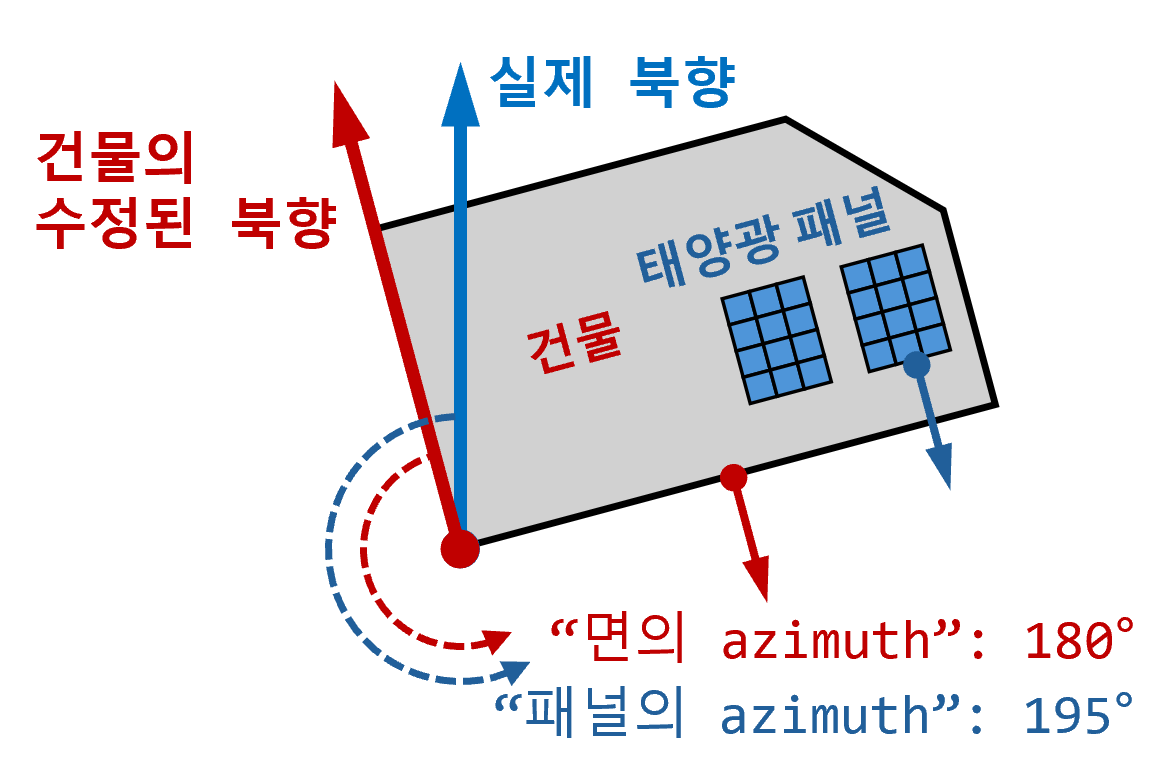
\includegraphics{태양광패널의 azimuth 설명.png}
  \caption{태양광 패널의 \texttt{azimuth}}
  \label{fig:azimuth_of_PVpanel}
\end{defaultfigure}

\paragraph{tilt} 패널의 경사각. 0$^\circ$는 수평면, 90$^\circ$는 수직면을 의미한다.

\subsubsection{profile} \label{subsubsection:ioref:profile}
존의 내부부하 및 발열을 나타내는 프로필이다.

\jsontable{profile}{
  \jsontablerow{id             }{\TypeTag{S}}{\ReqTag{R}}{}{}{}{}
  \jsontablerow{name           }{\TypeTag{S}}{\ReqTag{R}}{}{}{}{}
  \jsontablerow{hvac_availability_id}{\TypeTag{S}}{\ReqTag{R}}{}{}{\hyperref[subsubsection:ioref:schedule]{\texttt{schedule}}의 \texttt{id}}{}
  \jsontablerow{hotwater_id}{\TypeTag{S}}{\ReqTag{O}}{\texttt{null}}{}{\hyperref[subsubsection:ioref:schedule]{\texttt{schedule}}의 \texttt{id}}{}
  \jsontablerow{occupant_id}{\TypeTag{S}}{\ReqTag{O}}{\texttt{null}}{}{\hyperref[subsubsection:ioref:schedule]{\texttt{schedule}}의 \texttt{id}}{}
  \jsontablerow{lighting_id}{\TypeTag{S}}{\ReqTag{O}}{\texttt{null}}{}{\hyperref[subsubsection:ioref:schedule]{\texttt{schedule}}의 \texttt{id}}{}
  \jsontablerow{equipment_id}{\TypeTag{S}}{\ReqTag{O}}{\texttt{null}}{}{\hyperref[subsubsection:ioref:schedule]{\texttt{schedule}}의 \texttt{id}}{}
  \jsontablerow{heating_setpoint_id }{\TypeTag{S}}{\needtobeexplain}{\texttt{null}}{}{\hyperref[subsubsection:ioref:schedule]{\texttt{schedule}}의 \texttt{id}}{}
  \jsontablerow{cooling_setpoint_id }{\TypeTag{S}}{\needtobeexplain}{\texttt{null}}{}{\hyperref[subsubsection:ioref:schedule]{\texttt{schedule}}의 \texttt{id}}{}
}

\paragraph{id} 프로필의 식별자. \ref{subsubsection:ioref:id_description}에 따라 정의된다.

\paragraph{name} 사용자 편의를 위해 제공되는 프로필 구별 식별자. 중복, 사용가능한 문자에 제한이 없으며, 시뮬레이션에 직접 사용되지 않는다.

\paragraph{hvac\_availability\_id} 설비 운영 프로필의 식별자.

\paragraph{hotwater\_id} 급탕부하 스케줄. 해당 값을 입력하지 않을 경우 (\texttt{null}), 급탕부하가 없는 것으로 취급된다.

\paragraph{occupant\_id} 인체발열 스케줄. 해당 값을 입력하지 않을 경우 (\texttt{null}), 인체발열이 없는 것으로 취급된다.

\paragraph{lighting\_id} 조명발열 스케줄. 해당 값을 입력하지 않을 경우 (\texttt{null}), 조명발열이 없는 것으로 취급된다.

\paragraph{equipment\_id} 기기발열 스케줄. 해당 값을 입력하지 않을 경우 (\texttt{null}), 기기발열이 없는 것으로 취급된다.

\paragraph{heating\_setpoint\_id} 난방 설정온도 스케줄. 난방 설비를 가동하는 경우(\texttt{hvac\_availability\_id}의 모든 값이 0이 아닐 때)요구된다.

\paragraph{cooling\_setpoint\_id} 냉방 설정온도 스케줄. 냉방 설비를 가동하는 경우(\texttt{hvac\_availability\_id}의 모든 값이 0이 아닐 때)요구된다.

\subsubsection{profile\_component} \label{subsubsection:ioref:profile_component}
프로필을 구성하는 각 요소들(\texttt{scheduels},\texttt{rulesets},\texttt{day\_schedules})을 포함하는 개체이다.

\jsontable{profile\_component}{
  \jsontablerow{schedules    }{[ \hyperref[subsubsection:ioref:schedule]{\texttt{schedule}} ]}{\ReqTag{R}}{}{}{[0, $Inf$)}{}
  \jsontablerow{rulesets     }{[ \hyperref[subsubsection:ioref:ruleset]{\texttt{ruleset}} ]}{\ReqTag{R}}{}{}{[0, $Inf$)}{}
  \jsontablerow{day_schedules}{[ \hyperref[subsubsection:ioref:dayschedule]{\texttt{day\_schedule}} ]}{\ReqTag{R}}{}{}{[0, $Inf$)}{}
}

\subsubsection{schedule} \label{subsubsection:ioref:schedule}
ㅁㅁ
\jsontable{schedule}{
  \jsontablerow{id     }{\TypeTag{S}}{\ReqTag{R}}{}{}{}{}
  \jsontablerow{name   }{\TypeTag{S}}{\ReqTag{R}}{}{}{}{}
  \jsontablerow{periods}{[ \hyperref[subsubsection:ioref:period]{\texttt{period}} ]}{\ReqTag{R}}{}{}{}{}
}

\paragraph{id} 스케줄의 식별자. \ref{subsubsection:ioref:id_description}에 따라 정의된다.

\paragraph{name} 사용자 편의를 위해 제공되는 스케줄 구별 식별자. 중복, 사용가능한 문자에 제한이 없으며, 시뮬레이션에 직접 사용되지 않는다.

\subsubsection{period} \label{subsubsection:ioref:period}
주간 규칙을 적용할 기간을 명시한다.
\jsontable{period}{
  \jsontablerow{start     }{\TypeTag{S}}{\ReqTag{R}}{}{}{\needtobeexplain}{}
  \jsontablerow{end       }{\TypeTag{S}}{\ReqTag{R}}{}{}{\needtobeexplain}{}
  \jsontablerow{ruleset_id}{\TypeTag{S}}{\ReqTag{R}}{}{}{\hyperref[subsubsection:ioref:ruleset]{\texttt{ruleset}}의 \texttt{id}}{}
}

\paragraph{start} 기간이 시작하는 날짜. ``MM/DD''의 형태로 표기한다(예: 3월 17일 $\rightarrow$ ``03/17''). 참고로, 입력한 날짜는 기간에 포함된다.

\paragraph{end} 기간이 끝나는 날짜. ``MM/DD''의 형태로 표기한다(예: 3월 17일 $\rightarrow$ ``03/17''). 참고로, 입력한 날짜는 기간에 포함된다.

\paragraph{ruleset\_id} 적용할 주간 규칙의 ID.

\subsubsection{ruleset} \label{subsubsection:ioref:ruleset}
주간 규칙이다.
\jsontable{ruleset}{
  \jsontablerow{id          }{\TypeTag{S}}{\ReqTag{R}}{}{}{}{}
  \jsontablerow{name        }{\TypeTag{S}}{\ReqTag{R}}{}{}{}{}
  \jsontablerow{weekdays_id }{\TypeTag{S}}{\ReqTag{R}}{}{}{\hyperref[subsubsection:ioref:dayschedule]{\texttt{day\_schedule}}의 \texttt{id}}{}
  \jsontablerow{weekends_id }{\TypeTag{S}}{\ReqTag{R}}{}{}{\hyperref[subsubsection:ioref:dayschedule]{\texttt{day\_schedule}}의 \texttt{id}}{}
  \jsontablerow{monday_id   }{\TypeTag{S}}{\ReqTag{O}}{\texttt{null}}{}{\hyperref[subsubsection:ioref:dayschedule]{\texttt{day\_schedule}}의 \texttt{id}}{}
  \jsontablerow{tuesday_id  }{\TypeTag{S}}{\ReqTag{O}}{\texttt{null}}{}{\hyperref[subsubsection:ioref:dayschedule]{\texttt{day\_schedule}}의 \texttt{id}}{}
  \jsontablerow{wednesday_id}{\TypeTag{S}}{\ReqTag{O}}{\texttt{null}}{}{\hyperref[subsubsection:ioref:dayschedule]{\texttt{day\_schedule}}의 \texttt{id}}{}
  \jsontablerow{thursday_id }{\TypeTag{S}}{\ReqTag{O}}{\texttt{null}}{}{\hyperref[subsubsection:ioref:dayschedule]{\texttt{day\_schedule}}의 \texttt{id}}{}
  \jsontablerow{friday_id   }{\TypeTag{S}}{\ReqTag{O}}{\texttt{null}}{}{\hyperref[subsubsection:ioref:dayschedule]{\texttt{day\_schedule}}의 \texttt{id}}{}
  \jsontablerow{saturday_id }{\TypeTag{S}}{\ReqTag{O}}{\texttt{null}}{}{\hyperref[subsubsection:ioref:dayschedule]{\texttt{day\_schedule}}의 \texttt{id}}{}
  \jsontablerow{sunday_id   }{\TypeTag{S}}{\ReqTag{O}}{\texttt{null}}{}{\hyperref[subsubsection:ioref:dayschedule]{\texttt{day\_schedule}}의 \texttt{id}}{}
}

\paragraph{id} 주간규칙의 식별자. \ref{subsubsection:ioref:id_description}에 따라 정의된다.

\paragraph{name} 사용자 편의를 위해 제공되는 주간규칙 구별 식별자. 중복, 사용가능한 문자에 제한이 없으며, 시뮬레이션에 직접 사용되지 않는다.

\paragraph{weekdays\_id} 주중(월-금)에 적용되는 일간스케줄.

\paragraph{weekends\_id} 주말(토,일)에 적용되는 일간스케줄.

\paragraph{monday\_id} 월요일에 적용되는 일간스케줄. \texttt{null}이 아닌 경우, \texttt{weekdays\_id}보다 우선하여 적용된다.

\paragraph{tuesday\_id} 화요일에 적용되는 일간스케줄. \texttt{null}이 아닌 경우, \texttt{weekdays\_id}보다 우선하여 적용된다.

\paragraph{wednesday\_id} 수요일에 적용되는 일간스케줄. \texttt{null}이 아닌 경우, \texttt{weekdays\_id}보다 우선하여 적용된다.

\paragraph{thursday\_id} 목요일에 적용되는 일간스케줄. \texttt{null}이 아닌 경우, \texttt{weekdays\_id}보다 우선하여 적용된다.

\paragraph{friday\_id} 금요일에 적용되는 일간스케줄. \texttt{null}이 아닌 경우, \texttt{weekdays\_id}보다 우선하여 적용된다.

\paragraph{saturday\_id} 토요일에 적용되는 일간스케줄. \texttt{null}이 아닌 경우, \texttt{weekends\_id}보다 우선하여 적용된다.

\paragraph{sunday\_id} 일요일에 적용되는 일간스케줄. \texttt{null}이 아닌 경우, \texttt{weekends\_id}보다 우선하여 적용된다.

\paragraph{holiday\_id} 공휴일에 적용되는 일간스케줄. \texttt{null}인 경우, \texttt{sunday\_id}의 일간스케줄이 기본으로 적용된다.

\subsubsection{day\_schedule} \label{subsubsection:ioref:dayschedule}
일간스케줄이다.
\jsontable{day\_schedule}{
  \jsontablerow{id    }{\TypeTag{S}}{\ReqTag{R}}{}{}{}{}
  \jsontablerow{name  }{\TypeTag{S}}{\ReqTag{R}}{}{}{}{}
  \jsontablerow{type  }{\TypeTag{E}}{\ReqTag{R}}{}{}{}{}
  \jsontablerow{values}{[ \TypeTag{F} ]}{\ReqTag{R}}{}{}{144}{}
}

\paragraph{id} 일간스케줄의 식별자. \ref{subsubsection:ioref:id_description}에 따라 정의된다.

\paragraph{name} 사용자 편의를 위해 제공되는 일간스케줄 구별 식별자. 중복, 사용가능한 문자에 제한이 없으며, 시뮬레이션에 직접 사용되지 않는다.

\paragraph{type} 일간스케줄 종류. 시뮬레이션에 직접 사용되지 않는다.

\paragraph{values} 시간별 스케줄 값. 각 값은 10분간의 값을 의미하며, 크기가 144개인 시간별 값(array)로 입력한다(1일;24시간;1440분).

\subsubsection{material} \label{subsubsection:ioref:material}

\jsontable{material}{
  \jsontablerow{id           }{\TypeTag{S}}{\ReqTag{R}}{}{}{}{}
  \jsontablerow{name         }{\TypeTag{S}}{\ReqTag{R}}{}{}{}{}
  \jsontablerow{conductivity }{\TypeTag{F}}{\ReqTag{R}}{}{}{}{W{\cdot}m^{-1}{\cdot}K^{-1}}
  \jsontablerow{density      }{\TypeTag{F}}{\ReqTag{R}}{}{}{}{kg{\cdot}m^{-3}}
  \jsontablerow{specific_heat}{\TypeTag{F}}{\ReqTag{R}}{}{}{(100,$Inf$)}{J{\cdot}kg^{-1}{\cdot}K^{-1}}
}

\paragraph{id} 재료의 식별자. \ref{subsubsection:ioref:id_description}에 따라 정의된다.

\paragraph{name} 사용자 편의를 위해 제공되는 재료 구별 식별자. 중복, 사용가능한 문자에 제한이 없으며, 시뮬레이션에 직접 사용되지 않는다.

\paragraph{conductivity} 열전도율. 재료의 단위 두께를 통한 열 전달 능력을 나타낸다.

\paragraph{density} 밀도. 재료의 단위 부피당 질량을 나타낸다.

\paragraph{specific\_heat} 비열. 재료의 단위 질량이 1K 상승할 때 필요한 열량을 나타낸다.

\subsubsection{surface\_construction} \label{subsubsection:ioref:construction}

\jsontable{surface\_construction}{
  \jsontablerow{id    }{\TypeTag{S}}{\ReqTag{R}}{}{}{}{}
  \jsontablerow{name  }{\TypeTag{S}}{\ReqTag{R}}{}{}{}{}
  \jsontablerow{layers}{[ \hyperref[subsubsection:ioref:layer]{\texttt{layer}} ]}{\ReqTag{R}}{}{}{[1, 10]}{}
}
 
\paragraph{id} 레이어의 식별자. \ref{subsubsection:ioref:id_description}에 따라 정의된다.

\paragraph{name} 사용자 편의를 위해 제공되는 레이어 구별 식별자. 중복, 사용가능한 문자에 제한이 없으며, 시뮬레이션에 직접 사용되지 않는다.

\subsubsection{layer} \label{subsubsection:ioref:layer}

 \jsontable{layer}{
  \jsontablerow{material_id}{\TypeTag{S}}{\ReqTag{R}}{}{}{\hyperref[subsubsection:ioref:material]{\texttt{material}}의 \texttt{id}}{}
  \jsontablerow{thicknes   }{\TypeTag{F}}{\ReqTag{R}}{}{}{(0.003,$Inf$)}{m}
}

\paragraph{material\_id} 레이어 구성 재료의 ID.

\paragraph{thickness} 레이어 구성 재료의 두께.

\subsubsection{fenestration\_construction} \label{subsubsection:ioref:fenestrationconstruction}

\jsontable{fenestration\_construction}{
  \jsontablerow{id            }{\TypeTag{S}}{\ReqTag{R}}{}{}{}{}
  \jsontablerow{name          }{\TypeTag{S}}{\ReqTag{R}}{}{}{}{}
  \jsontablerow{is_transparent}{\TypeTag{B}}{\ReqTag{R}}{}{}{}{}
  \jsontablerow{u             }{\TypeTag{F}}{\ReqTag{R}}{}{}{(0, $Inf$)}{W{\cdot}m^{-1}{\cdot}K^{-1}}
  \jsontablerow{g             }{\TypeTag{F}}{\ReqTag{CR}}{}{\texttt{is\_transparent} = \texttt{True}}{(0,1]}{}
}

\paragraph{id} 창호의 식별자. \ref{subsubsection:ioref:id_description}에 따라 정의된다.

\paragraph{name} 사용자 편의를 위해 제공되는 창호 구별 식별자. 중복, 사용가능한 문자에 제한이 없으며, 시뮬레이션에 직접 사용되지 않는다.

\paragraph{is\_transparent} 구조체의 투명여부. 투명한 구조체의 개구부(예: 유리창, 유리문 등)는 ``True''로 입력하며, 불투명한 구조체의 개구부(예: 방화문, 나무문 등)는 ``False''로 입력한다.

\paragraph{u} 창호의 열관류율(U-value).

\paragraph{g} 창호의 열취득계수(G-value, SHGC).

% ---------------------------------------------------------------------------- %
%                                  NEW SECTION                                 %
% ---------------------------------------------------------------------------- %

\section{grexcel 구조 (.xlsx 파일)}
\subsection{개발규칙}
\texttt{grexcel}은 사용자에게 가장 친숙한 워크시트 도구인 Excel을 기반으로 
기본적인 데이터 입력 인터페이스(UI) 역할을 한다. 사용자가 한 페이지 내에서 많은 정보를 확인할 수 있도록 구성되어 있다.
\par
@TODO 
단위도 사용자에게 편한 단위 쓴다. 파란색은 뭐 초록색은 뭐... (@memo 정보 제공 파트에 집중하여 작성)

\subsection{sheet별 명세}
\subsubsection{건물정보}
@TODO

\subsubsection{실}
@TODO

\subsubsection{면}
@TODO

\subsubsection{개구부}
@TODO

\subsubsection{구조체\_면}
@TODO

\subsubsection{구조체\_개구부}
@TODO

\subsubsection{구조체\_면}
@TODO

\subsection{재료}
@TODO

\subsection{공급설비}
@TODO

\subsection{생산설비}
@TODO

\subsection{환기설비}
@TODO

\subsection{PV패널}
@TODO

\subsection{예시}
@TODO


\subsection{grexcel을 grjson으로 변환하는 과정}
유효한 컬럼만 떼고...
컬럼명에서 단위 없애고...
단위변환하고...
값변환할 것 하고...
@TODO  코드 풀어서 설명, 캡쳐 사진 넣기


% ---------------------------------------------------------------------------- %
%                                  NEW SECTION                                 %
% ---------------------------------------------------------------------------- %

\section{grresult 구조 (.grr 파일)}
\subsection{class별 명세}
\subsubsection{입력정보 및 계산 방식 관련}
\paragraph{building} 건물 관련 기본 정보를 포함한다.
\begin{itemize}
  \item \textbf{total\_area}: 면적당 지표 계산에 사용되는 건물의 연면적($m^2$)을 의미한다. 연면적의 정의는 \ref{subsec:floorarea_definition_for_EUI}에서 기술한다.
\end{itemize}

\paragraph{constants} 연료별, 용도별, 월별 에너지소요량으로부터, 1차에너지소요량(site2source, $kWh/kWh$), 온실가스 배출량(site2co2, $kgCO_{2,eq}/kWh$) 및 에너지요금(site2cost, $won/kWh$)을 계산하는 데 사용된 변환계수를 포함한다. 각 변환계수의 산출 과정에 대하여는 \ref{subsec:result_converting_coeff_definition}에서 기술한다.

\subsubsection{원시데이터 관련}
에너지소요량을 비롯한 4가지 지표는 용도별 (6가지), 열원별 (4가지), 월별 (12개월)로 제시된다.
\begin{itemize}
  \item 6가지 용도: 난방(heating), 냉방(cooling), 조명(lighting), 팬/펌프/전열교환기(circulation), 급탕(hotwater), 발전(generators)
  \item 5가지 열원: 전기(ELECTRICITY), 천연가스(NATURALGAS), 등유(OIL), 지역난방(DISTRICTHEATING)
\end{itemize}

\paragraph{site\_uses} 건물에서 쓰는거 월별로 원별로 용도별로. 이런식으로 구성되어있음.
\paragraph{source\_uses} 1차에너지에 해당하는 것.
\paragraph{co2} CO2 배출량
\paragraph{cost} 비용. 여기까지 다 site\_uses에다가 곱해서 얻어지는 것임

\subsubsection{요약데이터 관련}
\paragraph{summary\_per\_area} 다 합한 것.
\paragraph{summary\_gross} 에 면적을 곱한 것. 비용 관련된 부분은 얘를 보는 게 맞을 듯.

\subsection{예시}

아래는 결과 파일 예시이다.

\subsection{다른 도구와의 관계}
\subsubsection{EnergyPlus(IDFEditor, DesignBuilder, ...)}
이걸 좀 더 사용자 친화적으로 바꾼 개념임. 형상은 이렇게 이해하면 되고 설비는 이렇게 이해해야 함. EP 설비할 때는 이런걸 이렇게 신경썼을텐데 이 툴을 쓸 때는 이런식으로 접근하면 대응되게 할 수 있음.

>> 이거 레벨 한단계 안올리면 결과파일 관련 내용임

\subsubsection{ECO2}
입력체계는 거의 비슷하다. 원래 하던대로 하면 된다. 단 형상쪽은 좀 주의해야 할 것임. \par
결과도 비슷한데 환기쪽만 조심하면 됨. ECO2에서 환기는 환기침기부하지만 우리는 그런거 없음. 환기침기부하생기면 냉난방으로 처리하는 거니까 냉난방에 묶여있음. 써큘레이션이라고 팬 펌프 전열교환기만 따로 뽑았음.

>> 이거 레벨 한단계 안올리면 결과파일 관련 내용임
% chap2.tex
\part{시뮬레이션 알고리즘}
\label{part:algorithm}

% ---------------------------------------------------------------------------- %
%                                  NEW SECTION                                 %
% ---------------------------------------------------------------------------- %

\chapter{시뮬레이션의 절차 및 구조}

\section{데이터 변환 시뮬레이션의 순서}

\subsection{시뮬레이션 개요}
시뮬레이션을 하려면, 입력데이터를 읽고 변환하고 옵션 설정해서 \ep 돌리고 결과 나온거 정리해서 반환한다.

데이터를 읽고, 요구하는 json 파일로 변환하는 과정이 필요함. 이렇게 해서 json을 입력하면 \simulator 엔진으로 시뮬레이션을 수행하고, 결과를 불러와 사용자에게 보여주는 방식이다.

\subsection{데이터 체계}
json구조로 들어온 데이터는, 동일한 python 구조체로 변환되고 그게 dragon이라는 \eq 친화적 구조체로 변환된 다음 idf로 내보내진다.

% ---------------------------------------------------------------------------- %
%                                  NEW SECTION                                 %
% ---------------------------------------------------------------------------- %

\section{시뮬레이션 조건}
\subsection{기상데이터}
\subsubsection{주소 및 행정구역 기준}
주소 정보는 2024년 12월 31일 기준 행정구역 체계를 적용하였으며, 세종특별자치시와 제주특별자치도(제주시, 서귀포시)를 포함하여 전국을 총 229개 시·군·구로 분류하였다.
각 시·군·구의 중심 좌표는 Naver Cloud Platform(NCP)에서 제공하는 Geocoding API를 기반으로 한 \texttt{korean\_geocoding} Python 패키지를 활용하여 위도(latitude)와 경도(longitude) 정보를 추출하였다.

\subsubsection{기상데이터 수집}
기상데이터는 국제적으로 통용되는 기상데이터 플랫폼인 OneBuilding.org\cite{onebuilding2025}에서 제공하는 TMYx(Typical Meteorological Year) 데이터를 활용하였다. 해당 플랫폼은 각 지역별 기상데이터를 총 7개 형식(clm, ddy, epw, pvsyst, rain, stat, wea)으로 제공하며, 본 시뮬레이터에서는 EnergyPlus 시뮬레이션에 요구되는 EPW 형식을 사용한다.
\begin{itemize}
  \item 수집 대상: 전국 95개 기상지점
  \item 데이터 기간: 2009년 - 2023년
  \item 데이터 검토: 결측치 없음
\end{itemize}
\paragraph{tmy} TMYx(Typical Meteorological Year)는 ISO 15927-4를 기반으로 작성한 표준 기상데이터를 의미한다. ISO 15927-4 방법은 아래와 같은 절차로 이루어진다\cite{shimtmyx} (Figure \ref{fig:tmyxalgorithm})
\begin{enumerate}
  \item 지역별 데이터 수집 (시간별 건구온도, 상대습도, 수평면 전일사량, 풍속)
  \item 시간별 수집 데이터를 일 평균 데이터로 변환
  \item 하루평균 데이터를 long-term CDF(전체 수집 기간), monthly CDF로 구분하고, 건구온도, 상대습도, 수평면 전일사량의 누적분포 함수 계산 (FS방법)
  
\[ 
  FS_{x}(y,m) = \left(\frac{1}{n}\right) \sum_{i=1}^{n} |CDF_{m}(x_{i}) - CDF_{y,m}(x_{i})|
\]

  \item $FS_{x}(y,m)$의 값이 작은 순으로 월 별 3개 연도를 선정
  \item 장기 평균 풍속과 월별 평균 풍속의 편차가 가장 작은 해를 대표 해로 선정
\end{enumerate}

\begin{defaultfigure}
  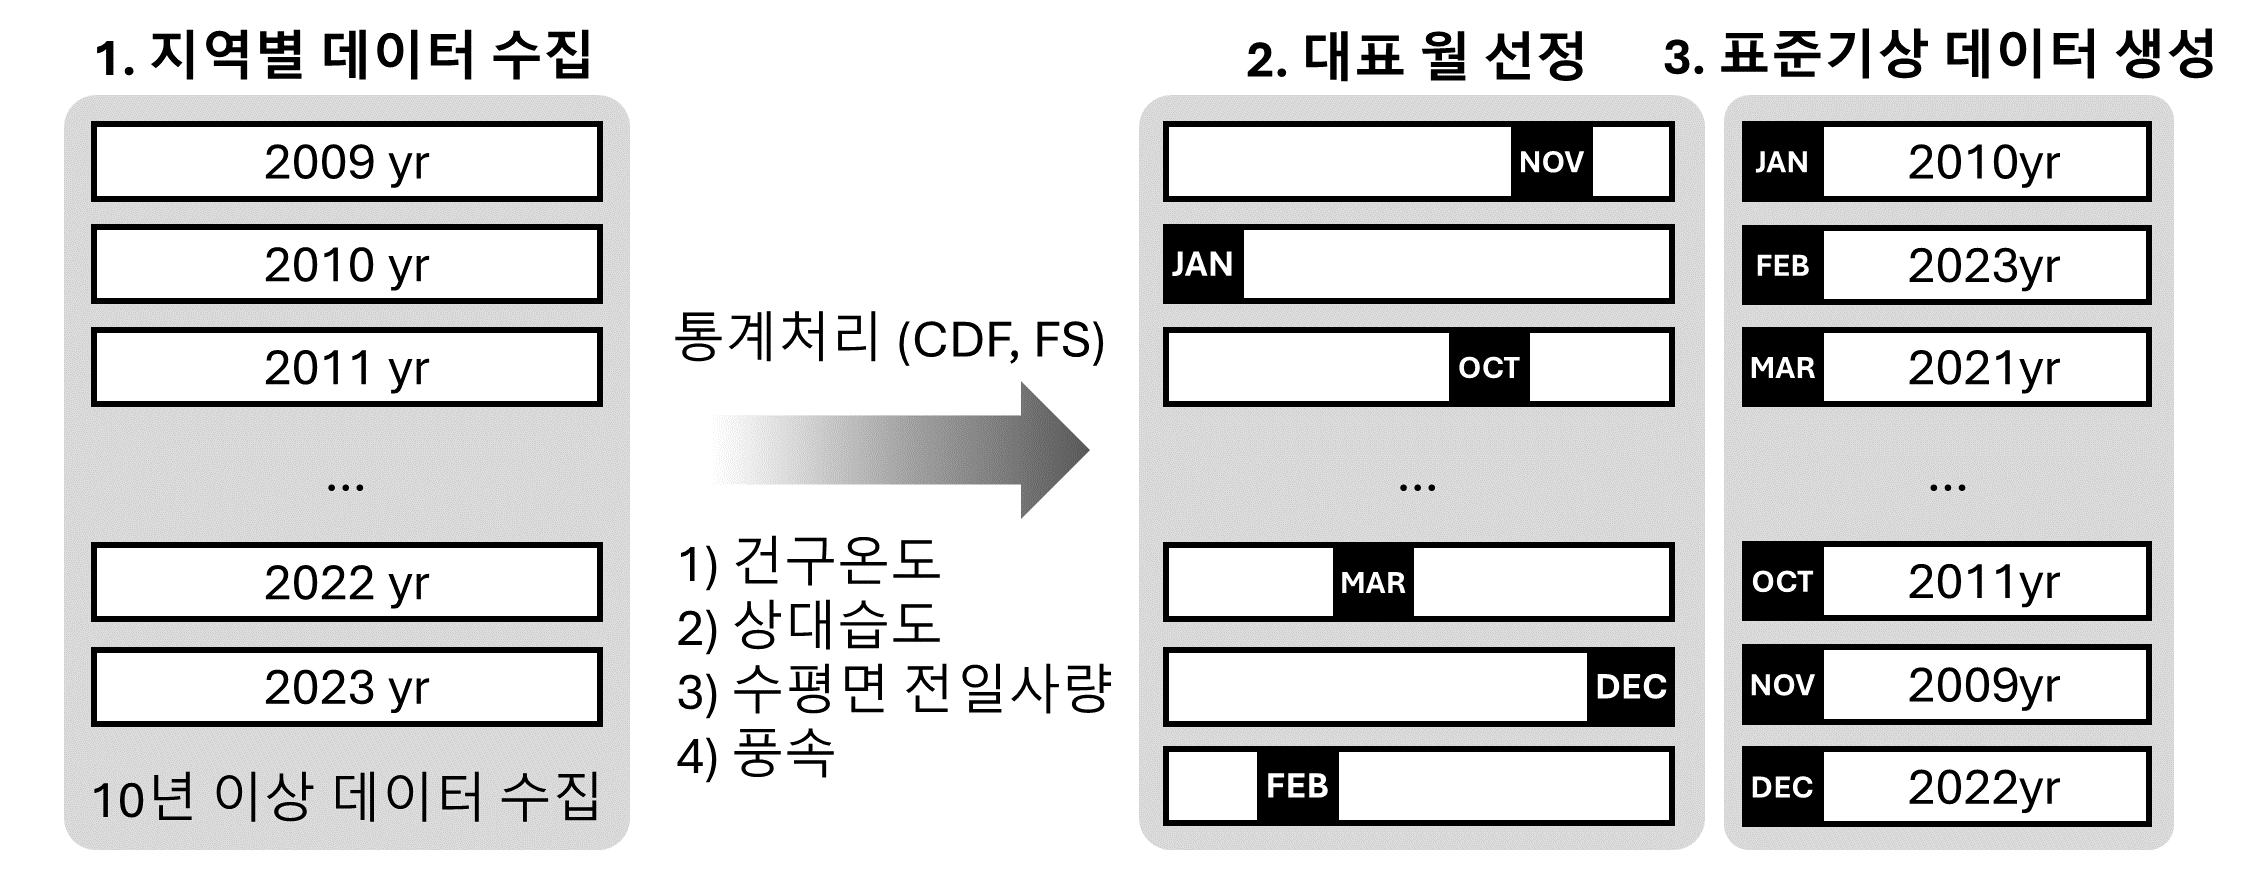
\includegraphics[width=\textwidth]{표준기상데이터생성.png}
  \caption{표준기상데이터 생성 방법 (ISO 15927-4)}
  \label{fig:tmyxalgorithm}
\end{defaultfigure}


\subsubsection{주소와 기상데이터 매칭방식}
\label{sec:address_weather_matching}
기상데이터 매칭은 각 시·군·구의 중심 좌표와 95개 TMY 기상지점의 위도·경도 정보를 비교하여, Haversine 공식을 이용한 거리 계산 결과 가장 가까운 지점을 선택하는 방식으로 매칭함. 
각 행정구역별 최근접 기상지점의 epw를 매칭한 결과는 표~\ref{tab:weather_mapping}에 제시함.

\renewcommand{\arraystretch}{0.8}
\begin{longtable}{lcclcc}
  \caption{행정구역별 기상데이터 매칭 결과} \\
  \label{tab:weather_mapping} \\
  \toprule
  \small
  시·군·구 & 위도[$^\circ$] & 경도[$^\circ$] & 매칭 EPW 지역명 & WMOcode & EPW 기준년도 \\ \midrule
  \endfirsthead
  \multicolumn{6}{r}{\textit{(이전 페이지에서 계속)}} \\ \toprule
  시·군·구 & 위도[$^\circ$] & 경도[$^\circ$] & 매칭 EPW 지역명 & WMOcode & EPW 기준년도 \\ \midrule
  \endhead
  \midrule \multicolumn{6}{r}{\textit{(다음 페이지에 계속)}} \\ \bottomrule
  \endfoot
  \bottomrule
  \endlastfoot
  % 본문 데이터 (예시)
  서울특별시 종로구 & 37.57 & 126.98 & Seoul.WS & 471080 & '09-'23 \\
  서울특별시 중구 & 37.56 & 127.00 & Seoul.WS & 471080 & '09-'23 \\
  서울특별시 용산구 & 37.53 & 126.99 & Seoul.WS & 471080 & '09-'23 \\
  서울특별시 성동구 & 37.56 & 127.04 & Seoul.WS & 471080 & '09-'23 \\
  서울특별시 광진구 & 37.54 & 127.08 & Seoul-Seongnam.AP & 471110 & '09-'23 \\
  서울특별시 동대문구 & 37.57 & 127.04 & Seoul.WS & 471080 & '09-'23 \\
  서울특별시 중랑구 & 37.61 & 127.09 & Seoul.WS & 471080 & '09-'23 \\
  서울특별시 성북구 & 37.59 & 127.02 & Seoul.WS & 471080 & '09-'23 \\
  서울특별시 강북구 & 37.64 & 127.03 & Seoul.WS & 471080 & '09-'23 \\
  서울특별시 도봉구 & 37.67 & 127.05 & Seoul.WS & 471080 & '09-'23 \\
  서울특별시 노원구 & 37.65 & 127.06 & Seoul.WS & 471080 & '09-'23 \\
  서울특별시 은평구 & 37.60 & 126.93 & Seoul.WS & 471080 & '09-'23 \\
  서울특별시 서대문구 & 37.58 & 126.94 & Seoul.WS & 471080 & '09-'23 \\
  서울특별시 마포구 & 37.57 & 126.90 & Seoul.WS & 471080 & '09-'23 \\
  서울특별시 양천구 & 37.52 & 126.87 & Gimpo.Intl.AP & 471100 & '09-'23 \\
  서울특별시 강서구 & 37.55 & 126.85 & Gimpo.Intl.AP & 471100 & '09-'23 \\
  서울특별시 구로구 & 37.50 & 126.89 & Seoul.WS & 471080 & '09-'23 \\
  서울특별시 금천구 & 37.46 & 126.90 & Seoul.WS & 471080 & '09-'23 \\
  서울특별시 영등포구 & 37.53 & 126.90 & Seoul.WS & 471080 & '09-'23 \\
  서울특별시 동작구 & 37.51 & 126.94 & Seoul.WS & 471080 & '09-'23 \\
  서울특별시 관악구 & 37.48 & 126.95 & Seoul.WS & 471080 & '09-'23 \\
  서울특별시 서초구 & 37.48 & 127.03 & Seoul-Seongnam.AP & 471110 & '09-'23 \\
  서울특별시 강남구 & 37.52 & 127.05 & Seoul.WS & 471080 & '09-'23 \\
  서울특별시 송파구 & 37.51 & 127.11 & Seoul-Seongnam.AP & 471110 & '09-'23 \\
  서울특별시 강동구 & 37.53 & 127.12 & Seoul-Seongnam.AP & 471110 & '09-'23 \\
  부산광역시 중구 & 35.11 & 129.03 & Busan-Daecheongdong.WS & 471590 & '09-'23 \\
  부산광역시 서구 & 35.10 & 129.02 & Busan-Daecheongdong.WS & 471590 & '09-'23 \\
  부산광역시 동구 & 35.13 & 129.05 & Busan-Daecheongdong.WS & 471590 & '09-'23 \\
  부산광역시 영도구 & 35.09 & 129.07 & Busan-Daecheongdong.WS & 471590 & '09-'23 \\
  부산광역시 부산진구 & 35.16 & 129.05 & Busan-Daecheongdong.WS & 471590 & '09-'23 \\
  부산광역시 동래구 & 35.20 & 129.09 & Busan-Daecheongdong.WS & 471590 & '09-'23 \\
  부산광역시 남구 & 35.14 & 129.08 & Busan-Daecheongdong.WS & 471590 & '09-'23 \\
  부산광역시 북구 & 35.20 & 128.99 & Busan-Gimhae.Intl.AP & 471530 & '09-'23 \\
  부산광역시 해운대구 & 35.16 & 129.16 & Busan-Daecheongdong.WS & 471590 & '09-'23 \\
  부산광역시 사하구 & 35.10 & 128.97 & Busan-Daecheongdong.WS & 471590 & '09-'23 \\
  부산광역시 금정구 & 35.24 & 129.09 & Busan-Gimhae.Intl.AP & 471530 & '09-'23 \\
  부산광역시 강서구 & 35.21 & 128.98 & Busan-Gimhae.Intl.AP & 471530 & '09-'23 \\
  부산광역시 연제구 & 35.18 & 129.08 & Busan-Daecheongdong.WS & 471590 & '09-'23 \\
  부산광역시 수영구 & 35.15 & 129.11 & Busan-Daecheongdong.WS & 471590 & '09-'23 \\
  부산광역시 사상구 & 35.15 & 128.99 & Busan-Gimhae.Intl.AP & 471530 & '09-'23 \\
  부산광역시 기장군 & 35.24 & 129.22 & Busan-Daecheongdong.WS & 471590 & '09-'23 \\
  대구광역시 중구 & 35.87 & 128.61 & Camp.Walker-Daegu & 471425 & '09-'23 \\
  대구광역시 동구 & 35.89 & 128.64 & Daegu.Intl.AP & 471420 & '09-'23 \\
  대구광역시 서구 & 35.87 & 128.56 & Camp.Walker-Daegu & 471425 & '09-'23 \\
  대구광역시 남구 & 35.85 & 128.60 & Camp.Walker-Daegu & 471425 & '09-'23 \\
  대구광역시 북구 & 35.89 & 128.58 & Camp.Walker-Daegu & 471425 & '09-'23 \\
  대구광역시 수성구 & 35.86 & 128.63 & Daegu & 471430 & '09-'23 \\
  대구광역시 달서구 & 35.83 & 128.53 & Camp.Walker-Daegu & 471425 & '09-'23 \\
  대구광역시 달성군 & 35.77 & 128.43 & Camp.Walker-Daegu & 471425 & '09-'23 \\
  대구광역시 군위군 & 36.24 & 128.57 & Gumi & 471540 & '09-'23 \\
  인천광역시 강화군 & 37.75 & 126.49 & Pyoripsan & 471084 & '09-'23 \\
  인천광역시 옹진군 & 37.45 & 126.64 & Incheon.WS & 471120 & '09-'23 \\
  인천광역시 중구 & 37.47 & 126.62 & Incheon.WS & 471120 & '09-'23 \\
  인천광역시 동구 & 37.47 & 126.64 & Incheon.WS & 471120 & '09-'23 \\
  인천광역시 미추홀구 & 37.46 & 126.65 & Incheon.WS & 471120 & '09-'23 \\
  인천광역시 연수구 & 37.41 & 126.68 & Incheon.WS & 471120 & '09-'23 \\
  인천광역시 남동구 & 37.45 & 126.73 & Incheon.WS & 471120 & '09-'23 \\
  인천광역시 부평구 & 37.51 & 126.72 & Gimpo.Intl.AP & 471100 & '09-'23 \\
  인천광역시 계양구 & 37.54 & 126.74 & Gimpo.Intl.AP & 471100 & '09-'23 \\
  인천광역시 서구 & 37.55 & 126.68 & Incheon.WS & 471120 & '09-'23 \\
  광주광역시 동구 & 35.15 & 126.92 & Gwangju & 471560 & '09-'23 \\
  광주광역시 서구 & 35.15 & 126.89 & Gwangju & 471560 & '09-'23 \\
  광주광역시 남구 & 35.13 & 126.90 & Gwangju & 471560 & '09-'23 \\
  광주광역시 북구 & 35.17 & 126.91 & Gwangju & 471560 & '09-'23 \\
  광주광역시 광산구 & 35.14 & 126.79 & Gwangju.AP & 471580 & '09-'23 \\
  대전광역시 동구 & 36.31 & 127.45 & Daejeon.WS & 471330 & '09-'23 \\
  대전광역시 중구 & 36.33 & 127.42 & Daejeon.WS & 471330 & '09-'23 \\
  대전광역시 서구 & 36.36 & 127.38 & Daejeon.WS & 471330 & '09-'23 \\
  대전광역시 유성구 & 36.36 & 127.36 & Daejeon.WS & 471330 & '09-'23 \\
  대전광역시 대덕구 & 36.35 & 127.42 & Daejeon.WS & 471330 & '09-'23 \\
  울산광역시 중구 & 35.57 & 129.33 & Ulsan & 471520 & '09-'23 \\
  울산광역시 남구 & 35.54 & 129.33 & Ulsan & 471520 & '09-'23 \\
  울산광역시 동구 & 35.50 & 129.42 & Ulsan & 471520 & '09-'23 \\
  울산광역시 북구 & 35.58 & 129.36 & Ulsan & 471520 & '09-'23 \\
  울산광역시 울주군 & 35.52 & 129.24 & Ulsan & 471520 & '09-'23 \\
  세종특별자치시 & 36.48 & 127.29 & Gongju & 692214 & '09-'23 \\
  경기도 수원시 & 37.26 & 127.03 & Suwon.AP & 471200 & '09-'23 \\
  경기도 고양시 & 37.66 & 126.83 & Gimpo.Intl.AP & 471100 & '09-'23 \\
  경기도 용인시 & 37.24 & 127.18 & Maesanri & 471205 & '09-'23 \\
  경기도 성남시 & 37.42 & 127.13 & Seoul-Seongnam.AP & 471110 & '09-'23 \\
  경기도 부천시 & 37.50 & 126.77 & Gimpo.Intl.AP & 471100 & '09-'23 \\
  경기도 화성시 & 37.20 & 126.83 & Suwon.WS & 471190 & '09-'23 \\
  경기도 안산시 & 37.32 & 126.83 & Suwon.WS & 471190 & '09-'23 \\
  경기도 남양주시 & 37.64 & 127.22 & Yangsu.Ri & 693594 & '09-'23 \\
  경기도 안양시 & 37.39 & 126.96 & Suwon.WS & 471190 & '09-'23 \\
  경기도 평택시 & 36.99 & 127.11 & Pyeongtaek.AP & 471270 & '09-'23 \\
  경기도 시흥시 & 37.38 & 126.80 & Incheon.WS & 471120 & '09-'23 \\
  경기도 파주시 & 37.76 & 126.78 & Paju & 470990 & '09-'23 \\
  경기도 의정부시 & 37.74 & 127.03 & Gwangjeok & 693604 & '09-'23 \\
  경기도 김포시 & 37.62 & 126.72 & Gimpo.Intl.AP & 471100 & '09-'23 \\
  경기도 광주시 & 37.43 & 127.26 & Maesanri & 471205 & '09-'23 \\
  경기도 광명시 & 37.48 & 126.86 & Gimpo.Intl.AP & 471100 & '09-'23 \\
  경기도 군포시 & 37.36 & 126.94 & Suwon.WS & 471190 & '09-'23 \\
  경기도 하남시 & 37.54 & 127.21 & Seoul-Seongnam.AP & 471110 & '09-'23 \\
  경기도 오산시 & 37.15 & 127.08 & Osan.AB & 471220 & '09-'23 \\
  경기도 양주시 & 37.79 & 127.05 & Gwangjeok & 693604 & '09-'23 \\
  경기도 이천시 & 37.27 & 127.44 & Icheon & 470970 & '09-'23 \\
  경기도 구리시 & 37.59 & 127.13 & Seoul.WS & 471080 & '09-'23 \\
  경기도 안성시 & 37.01 & 127.28 & Pyeongtaek.AP & 471270 & '09-'23 \\
  경기도 포천시 & 37.89 & 127.20 & Dongducheon & 470980 & '09-'23 \\
  경기도 의왕시 & 37.34 & 126.97 & Suwon.WS & 471190 & '09-'23 \\
  경기도 양평군 & 37.49 & 127.49 & Yeoju.Range & 471315 & '09-'23 \\
  경기도 여주시 & 37.30 & 127.60 & Icheon & 470970 & '09-'23 \\
  경기도 동두천시 & 37.90 & 127.06 & Dongducheon & 470980 & '09-'23 \\
  경기도 과천시 & 37.43 & 126.99 & Seoul-Seongnam.AP & 471110 & '09-'23 \\
  경기도 가평군 & 37.83 & 127.51 & Gapyeong & 692114 & '09-'23 \\
  경기도 연천군 & 38.10 & 127.07 & Cheorwon & 470950 & '09-'23 \\
  강원도 춘천시 & 37.88 & 127.73 & Chuncheon-Camp.Page.AP & 471040 & '09-'23 \\
  강원도 원주시 & 37.34 & 127.92 & Wonju.WS & 471140 & '09-'23 \\
  강원도 강릉시 & 37.75 & 128.88 & Gangneung & 471050 & '09-'23 \\
  강원도 동해시 & 37.52 & 129.11 & Donghae.Radar & 471060 & '09-'23 \\
  강원도 태백시 & 37.16 & 128.99 & Taebaek.Provincial.Park & 471223 & '09-'23 \\
  강원도 속초시 & 38.21 & 128.59 & Sokcho & 470900 & '09-'23 \\
  강원도 삼척시 & 37.45 & 129.17 & Donghae.Radar & 471060 & '09-'23 \\
  강원도 홍천군 & 37.70 & 127.89 & Hongchon & 693624 & '09-'23 \\
  강원도 횡성군 & 37.49 & 127.99 & Wonju.WS & 471140 & '09-'23 \\
  강원도 영월군 & 37.18 & 128.46 & Yeongwol.WS & 471210 & '09-'23 \\
  강원도 평창군 & 37.37 & 128.39 & Yeongwol.WS & 471210 & '09-'23 \\
  강원도 정선군 & 37.38 & 128.66 & Yeongwol.WS & 471210 & '09-'23 \\
  강원도 철원군 & 38.15 & 127.31 & Cheorwon & 470950 & '09-'23 \\
  강원도 화천군 & 38.11 & 127.71 & Sachang.Ri & 693614 & '09-'23 \\
  강원도 양구군 & 38.11 & 127.99 & Yanggu & 692094 & '09-'23 \\
  강원도 인제군 & 38.07 & 128.17 & Yanggu & 692094 & '09-'23 \\
  강원도 고성군 & 38.38 & 128.47 & Geojin & 470800 & '09-'23 \\
  강원도 양양군 & 38.08 & 128.62 & Yangyang.Intl.AP & 470920 & '09-'23 \\
  충청북도 청주시 & 36.64 & 127.49 & Cheongju.WS & 471310 & '09-'23 \\
  충청북도 충주시 & 36.99 & 127.93 & Jungwon.AB & 471250 & '09-'23 \\
  충청북도 제천시 & 37.13 & 128.19 & Yeongwol.WS & 471210 & '09-'23 \\
  충청북도 보은군 & 36.49 & 127.73 & Seongmu.AB & 471240 & '09-'23 \\
  충청북도 옥천군 & 36.31 & 127.57 & Daejeon.WS & 471330 & '09-'23 \\
  충청북도 영동군 & 36.18 & 127.78 & Chupungnyeong & 471350 & '09-'23 \\
  충청북도 증평군 & 36.79 & 127.58 & Cheongju.Intl.AP & 471280 & '09-'23 \\
  충청북도 진천군 & 36.86 & 127.44 & Cheonan & 471450 & '09-'23 \\
  충청북도 괴산군 & 36.82 & 127.79 & Jungwon.AB & 471250 & '09-'23 \\
  충청북도 음성군 & 36.94 & 127.69 & Jungwon.AB & 471250 & '09-'23 \\
  충청북도 단양군 & 36.98 & 128.37 & Yeongwol.WS & 471210 & '09-'23 \\
  충청남도 천안시 & 36.82 & 127.11 & Cheonan & 471450 & '09-'23 \\
  충청남도 공주시 & 36.45 & 127.12 & Gongju & 692214 & '09-'23 \\
  충청남도 보령시 & 36.33 & 126.61 & Boryeong & 471500 & '09-'23 \\
  충청남도 아산시 & 36.79 & 127.00 & Pyeongtaek.AP & 471270 & '09-'23 \\
  충청남도 서산시 & 36.78 & 126.45 & Seosan.WS & 471290 & '09-'23 \\
  충청남도 논산시 & 36.19 & 127.10 & Daejeon.WS & 471330 & '09-'23 \\
  충청남도 계룡시 & 36.27 & 127.25 & Daejeon.WS & 471330 & '09-'23 \\
  충청남도 당진시 & 36.89 & 126.65 & Seosan.WS & 471290 & '09-'23 \\
  충청남도 금산군 & 36.11 & 127.49 & Geumsan & 692244 & '09-'23 \\
  충청남도 부여군 & 36.28 & 126.91 & Boryeong & 471500 & '09-'23 \\
  충청남도 서천군 & 36.08 & 126.69 & Gunsan & 471400 & '09-'23 \\
  충청남도 청양군 & 36.46 & 126.80 & Boryeong & 471500 & '09-'23 \\
  충청남도 홍성군 & 36.60 & 126.66 & Seosan.WS & 471290 & '09-'23 \\
  충청남도 예산군 & 36.68 & 126.84 & Seosan.WS & 471290 & '09-'23 \\
  충청남도 태안군 & 36.75 & 126.30 & Seosan.WS & 471290 & '09-'23 \\
  전라북도 전주시 & 35.82 & 127.15 & Jeonju & 471460 & '09-'23 \\
  전라북도 군산시 & 35.97 & 126.74 & Gunsan & 471400 & '09-'23 \\
  전라북도 익산시 & 35.95 & 126.96 & Jeonju & 471460 & '09-'23 \\
  전라북도 정읍시 & 35.57 & 126.86 & Jeongeup & 471710 & '09-'23 \\
  전라북도 남원시 & 35.42 & 127.39 & Namwon & 471730 & '09-'23 \\
  전라북도 김제시 & 35.80 & 126.88 & Jeonju & 471460 & '09-'23 \\
  전라북도 완주군 & 35.90 & 127.16 & Jeonju & 471460 & '09-'23 \\
  전라북도 진안군 & 35.79 & 127.42 & Jeonju & 471460 & '09-'23 \\
  전라북도 무주군 & 36.01 & 127.66 & Geumsan & 692244 & '09-'23 \\
  전라북도 장수군 & 35.65 & 127.52 & Namwon & 471730 & '09-'23 \\
  전라북도 임실군 & 35.62 & 127.29 & Namwon & 471730 & '09-'23 \\
  전라북도 순창군 & 35.37 & 127.14 & Namwon & 471730 & '09-'23 \\
  전라북도 고창군 & 35.44 & 126.70 & Gochang & 471720 & '09-'23 \\
  전라북도 부안군 & 35.73 & 126.73 & Jeongeup & 471710 & '09-'23 \\
  전라남도 목포시 & 34.81 & 126.39 & Mokpo & 471650 & '09-'23 \\
  전라남도 여수시 & 34.76 & 127.66 & Yeosu.Obs & 471680 & '09-'23 \\
  전라남도 순천시 & 34.95 & 127.49 & Suncheon.WS & 471740 & '09-'23 \\
  전라남도 나주시 & 35.02 & 126.71 & Gwangju.AP & 471580 & '09-'23 \\
  전라남도 광양시 & 34.94 & 127.70 & Yeosu.AP & 471670 & '09-'23 \\
  전라남도 담양군 & 35.32 & 126.99 & Gwangju & 471560 & '09-'23 \\
  전라남도 곡성군 & 35.28 & 127.29 & Namwon & 471730 & '09-'23 \\
  전라남도 구례군 & 35.20 & 127.46 & Suncheon.WS & 471740 & '09-'23 \\
  전라남도 고흥군 & 34.60 & 127.28 & Yeosu.AP & 471670 & '09-'23 \\
  전라남도 보성군 & 34.77 & 127.08 & Suncheon.WS & 471740 & '09-'23 \\
  전라남도 화순군 & 35.06 & 126.99 & Gwangju & 471560 & '09-'23 \\
  전라남도 장흥군 & 34.68 & 126.91 & Wando.WS & 471700 & '09-'23 \\
  전라남도 강진군 & 34.64 & 126.77 & Wando.WS & 471700 & '09-'23 \\
  전라남도 해남군 & 34.57 & 126.60 & Wando.WS & 471700 & '09-'23 \\
  전라남도 영암군 & 34.80 & 126.70 & Mokpo & 471650 & '09-'23 \\
  전라남도 무안군 & 34.99 & 126.48 & Muan.Intl.AP & 471630 & '09-'23 \\
  전라남도 함평군 & 35.07 & 126.52 & Muan.Intl.AP & 471630 & '09-'23 \\
  전라남도 영광군 & 35.28 & 126.51 & Gochang & 471720 & '09-'23 \\
  전라남도 장성군 & 35.30 & 126.78 & Gwangju & 471560 & '09-'23 \\
  전라남도 완도군 & 34.31 & 126.75 & Wando.WS & 471700 & '09-'23 \\
  전라남도 진도군 & 34.49 & 126.26 & Jindo.WS & 471750 & '09-'23 \\
  전라남도 신안군 & 34.83 & 126.35 & Mokpo & 471650 & '09-'23 \\
  경상북도 포항시 & 36.02 & 129.34 & Pohang.WS & 471380 & '09-'23 \\
  경상북도 경주시 & 35.86 & 129.22 & Pohang.AP & 471390 & '09-'23 \\
  경상북도 김천시 & 36.14 & 128.11 & Chupungnyeong & 471350 & '09-'23 \\
  경상북도 안동시 & 36.57 & 128.73 & Andong.WS & 471360 & '09-'23 \\
  경상북도 구미시 & 36.12 & 128.34 & Gumi & 471540 & '09-'23 \\
  경상북도 영주시 & 36.81 & 128.62 & Andong.WS & 471360 & '09-'23 \\
  경상북도 영천시 & 35.97 & 128.94 & Daegu.Intl.AP & 471420 & '09-'23 \\
  경상북도 상주시 & 36.41 & 128.16 & Sangju.WS & 471370 & '09-'23 \\
  경상북도 문경시 & 36.59 & 128.19 & Yecheon.AP & 471340 & '09-'23 \\
  경상북도 경산시 & 35.83 & 128.74 & Daegu & 471430 & '09-'23 \\
  경상북도 의성군 & 36.35 & 128.70 & Andong.WS & 471360 & '09-'23 \\
  경상북도 청송군 & 36.44 & 129.06 & Andong.WS & 471360 & '09-'23 \\
  경상북도 영양군 & 36.67 & 129.11 & Andong.WS & 471360 & '09-'23 \\
  경상북도 영덕군 & 36.42 & 129.37 & Pohang.WS & 471380 & '09-'23 \\
  경상북도 청도군 & 35.65 & 128.73 & Cheongdo & 693414 & '09-'23 \\
  경상북도 고령군 & 35.73 & 128.26 & Camp.Walker-Daegu & 471425 & '09-'23 \\
  경상북도 성주군 & 35.92 & 128.28 & Gumi & 471540 & '09-'23 \\
  경상북도 칠곡군 & 36.00 & 128.40 & Gumi & 471540 & '09-'23 \\
  경상북도 예천군 & 36.65 & 128.44 & Yecheon.AP & 471340 & '09-'23 \\
  경상북도 봉화군 & 36.89 & 128.73 & Taebaek.Provincial.Park & 471223 & '09-'23 \\
  경상북도 울진군 & 36.99 & 129.40 & Uljin.WS & 471300 & '09-'23 \\
  경상북도 울릉군 & 37.48 & 130.91 & Ulleungdo.WS & 471150 & '09-'23 \\
  경상남도 창원시 & 35.23 & 128.68 & Changwon & 471550 & '09-'23 \\
  경상남도 진주시 & 35.18 & 128.11 & Jinju.WS & 471920 & '09-'23 \\
  경상남도 통영시 & 34.85 & 128.43 & Tongyeong.WS & 471620 & '09-'23 \\
  경상남도 사천시 & 35.00 & 128.06 & Sacheon.AB & 471610 & '09-'23 \\
  경상남도 김해시 & 35.23 & 128.89 & Busan-Gimhae.Intl.AP & 471530 & '09-'23 \\
  경상남도 밀양시 & 35.50 & 128.75 & Cheongdo & 693414 & '09-'23 \\
  경상남도 거제시 & 34.88 & 128.62 & Tongyeong.WS & 471620 & '09-'23 \\
  경상남도 양산시 & 35.34 & 129.04 & Busan-Gimhae.Intl.AP & 471530 & '09-'23 \\
  경상남도 의령군 & 35.32 & 128.26 & Jinju.WS & 471920 & '09-'23 \\
  경상남도 함안군 & 35.27 & 128.41 & Changwon & 471550 & '09-'23 \\
  경상남도 창녕군 & 35.54 & 128.49 & Cheongdo & 693414 & '09-'23 \\
  경상남도 고성군 & 34.97 & 128.32 & Tongyeong.WS & 471620 & '09-'23 \\
  경상남도 남해군 & 34.84 & 127.89 & Yeosu.Obs & 471680 & '09-'23 \\
  경상남도 하동군 & 35.07 & 127.75 & Jinju.WS & 471920 & '09-'23 \\
  경상남도 산청군 & 35.42 & 127.87 & Geochang.WS & 471570 & '09-'23 \\
  경상남도 함양군 & 35.52 & 127.73 & Geochang.WS & 471570 & '09-'23 \\
  경상남도 거창군 & 35.69 & 127.91 & Geochang.WS & 471570 & '09-'23 \\
  경상남도 합천군 & 35.57 & 128.17 & Geochang.WS & 471570 & '09-'23 \\
  제주특별자치도 제주시 & 33.50 & 126.53 & Jeju.WS & 471840 & '09-'23 \\
  제주특별자치도 서귀포시 & 33.25 & 126.56 & Seogwipo & 471890 & '09-'23 \\
\end{longtable}

\subsection{EnergyPlus 옵션} 시뮬레이션 옵션은 주로 건물의 전역 특성, 계산 시간 단위, 설비 용량 산정을 위한 부하 계산 조건 등이 있으며, 본 절에서는 주요 항목을 아래와 같이 정리한다.

\subsubsection{Building} 시뮬레이션 대상 건물의 특성을 정의하는 클래스이다. 본 매뉴얼에서는, 주요 항목만을 정리한다.
\paragraph[short]{Terrain} 건물이 위치한 주변 지형 조건을 정의한다. 이는, 외부 대류열전달계수와 풍속 등에 영향을 준다. 예를 들어, \texttt{Urban}은 주변이 빽빽한 도심 환경을 의미하고, \texttt{Country}는 개방된 농촌 지역을 의미한다. \simulator\는 기본값으로 \texttt{Suburbs}를 적용한다.
\paragraph[short]{Solar Distribution} 태양복사를 건물에 분배하는 방식을 정의하는 항목으로, 음영 효과를 무시하거나 외부·내부 음영 및 반사까지 고려하는 등 여러 수준의 방법을 선택할 수 있다. 
\simulator\는 형상 입력 방식을 \texttt{simplified geometry}로 채택하였으므로, 음영 효과를 무시하는 \texttt{MinimalShadowing} 옵션을 적용한다 (\cref{chap:simulator_geometry}).

\subsubsection{Timestep} 시뮬레이션의 기본 계산 시간 단위를 의미하며, 1시간(60분)을 몇 회로 분할하여 계산할 것인지 지정한다. 이 값은 실의 열 평형 계산(Zone Heat Balance)에서 열전달 및 부하 계산의 구동 시간 단위로 사용된다. 허용되는 입력 값은 4에서 60까지, 60을 정확히 나눌 수 있는 정수 (1, 2, 3, 4, 5, 6, 10, 12, 15, 20, 30, 60)이며, \ep\는 6(10분 단위 계산)을 권장한다 \cite{energyplusior242}. 더 낮은 값을 입력할 경우 연산 시간은 단축되나, 정확도가 저하될 수 있으며, \simulator\는 기본값으로 6을 적용한다. 

\subsubsection{DesignCondition} 냉·난방 부하 산정을 위해 기상데이터에서 대표적인 설계 조건을 정의하는 항목이다. 일반적으로 가장 더운 날(하계 설계일, SummerDesignDay)과 가장 추운 날(동계 설계일, WinterDesignDay)을 설계일로 지정하며, 사용자가 직접 조건을 입력하거나, 기상 파일(EPW)에 내장된 극한일(Extreme) 등의 데이터를 불러오는 방법도 활용할 수 있다 \cite{energyplusior242}.
\simulator 는 기상 파일(EPW)에 내장된 극한일(Extreme)을 설계 조건으로 정의함. @TODO


% ---------------------------------------------------------------------------- %
%                                  NEW SECTION                                 %
% ---------------------------------------------------------------------------- %

\section{EnergyPlus 구동}
\subsection{EnergyPlus 실행}
\subsubsection{EnergyPlus의 독립 구동 방법}
EnergyPlus는 EnergyPlus.exe를 직접 실행한다.

\subsection{디렉토리 구조}
코드 내부적으로는 그림()과 같은 구조로 호출하고 있다.
디렉토리는 중간에 3개의 temp 폴더가 생긴다.
temp 폴더 경로는 C:/users/.../Appdata/Local/Temp/하위에 생긴다.

% ---------------------------------------------------------------------------- %
%                                  NEW SECTION                                 %
% ---------------------------------------------------------------------------- %

\section{오류의 정의와 처리}
오류가 날 수도 있는데, 분류별로 보면 입력이 잘못된 경우와 뭐가 잘못된 경우와... \dots
각각에 대하여는 이렇게 이렇게 처리할 수 있다.

\subsection{입력변수가 잘못된 경우}
입력변수 오류는 python 객체로 전환될 때 탐지해서 ...하는 방식으로 반환한다. 사용자는 이걸 보고 무엇을 판단할 수 있다.

\subsection{idf 변환 과정이 잘못된 경우}

\subsection{EP가 안돌아가는 경우}

% ---------------------------------------------------------------------------- %
%                                  NEW SECTION                                 %
% ---------------------------------------------------------------------------- %

\chapter{항목별 idf 변환 방법}
\label{chap:simulator_geometry}

\section{형상 변환 알고리즘}

\subsection{EnergyPlus의 형상 입력 방식}

\subsubsection{형상 정보와 부하 계산 사이의 관계}

형상 정보는 실--외부, 실--실 사이 열교환, 일사 부하 등을 위해 필수적인 정보이다. EnergyPlus는 Figure \ref{fig:geometry_mechanism}\과 같이 면 단위로  면을 통해 이뤄진다. 이때 열교환에 영향을 미치는 면의 속성들은 아래와 같다. 일사부하 계산 시 음영효과 반영을 제외하면 실의 부하 계산을 위한 열평형 방정식에서 면들의 구체적인 좌푯값은 필수적이지 않으며, 면적으로 대체 가능함을 시사한다(Figure \ref{fig:geometry_mechanism2}).

\begin{itemize}
  \item 면과 외기와의 열교환 (\underline{면적}, 대류 열전달 계수, u값 등)
  \item 면 일사 부하 (\underline{면적}, 방위각, 음영효과, 흡수율 등)
  \item 실 공기와의 열교환 (\underline{면적}, 대류 열전달 계수)
  \item 개구부를 통한 일사부하 (\underline{면적}, 태양열 취득률)
\end{itemize}

\begin{defaultfigure}
  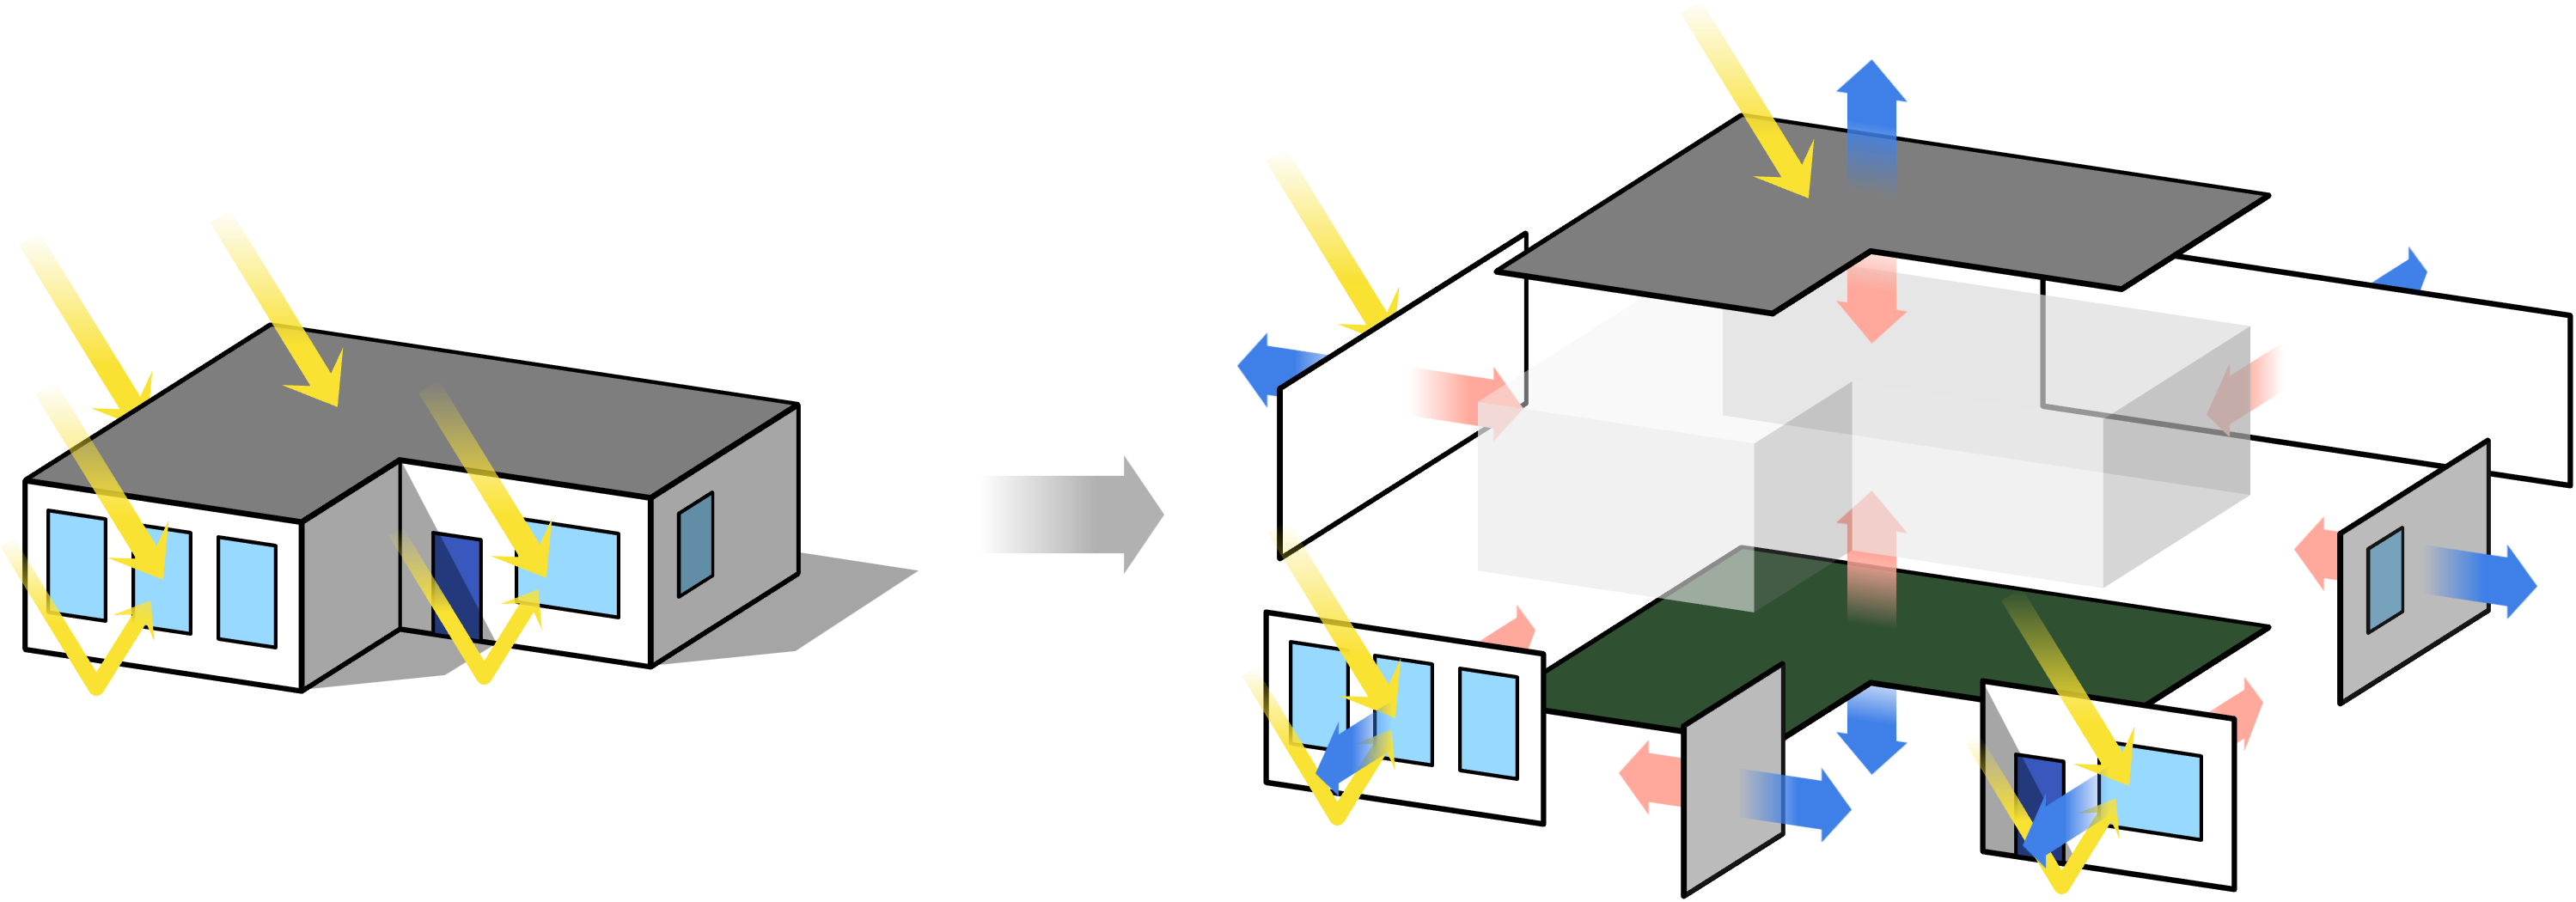
\includegraphics[width=0.8\textwidth]{geometry_mechanism.png}
  \caption{면을 통한 열교환 도식화}
  \label{fig:geometry_mechanism}
\end{defaultfigure}

\begin{defaultfigure}
  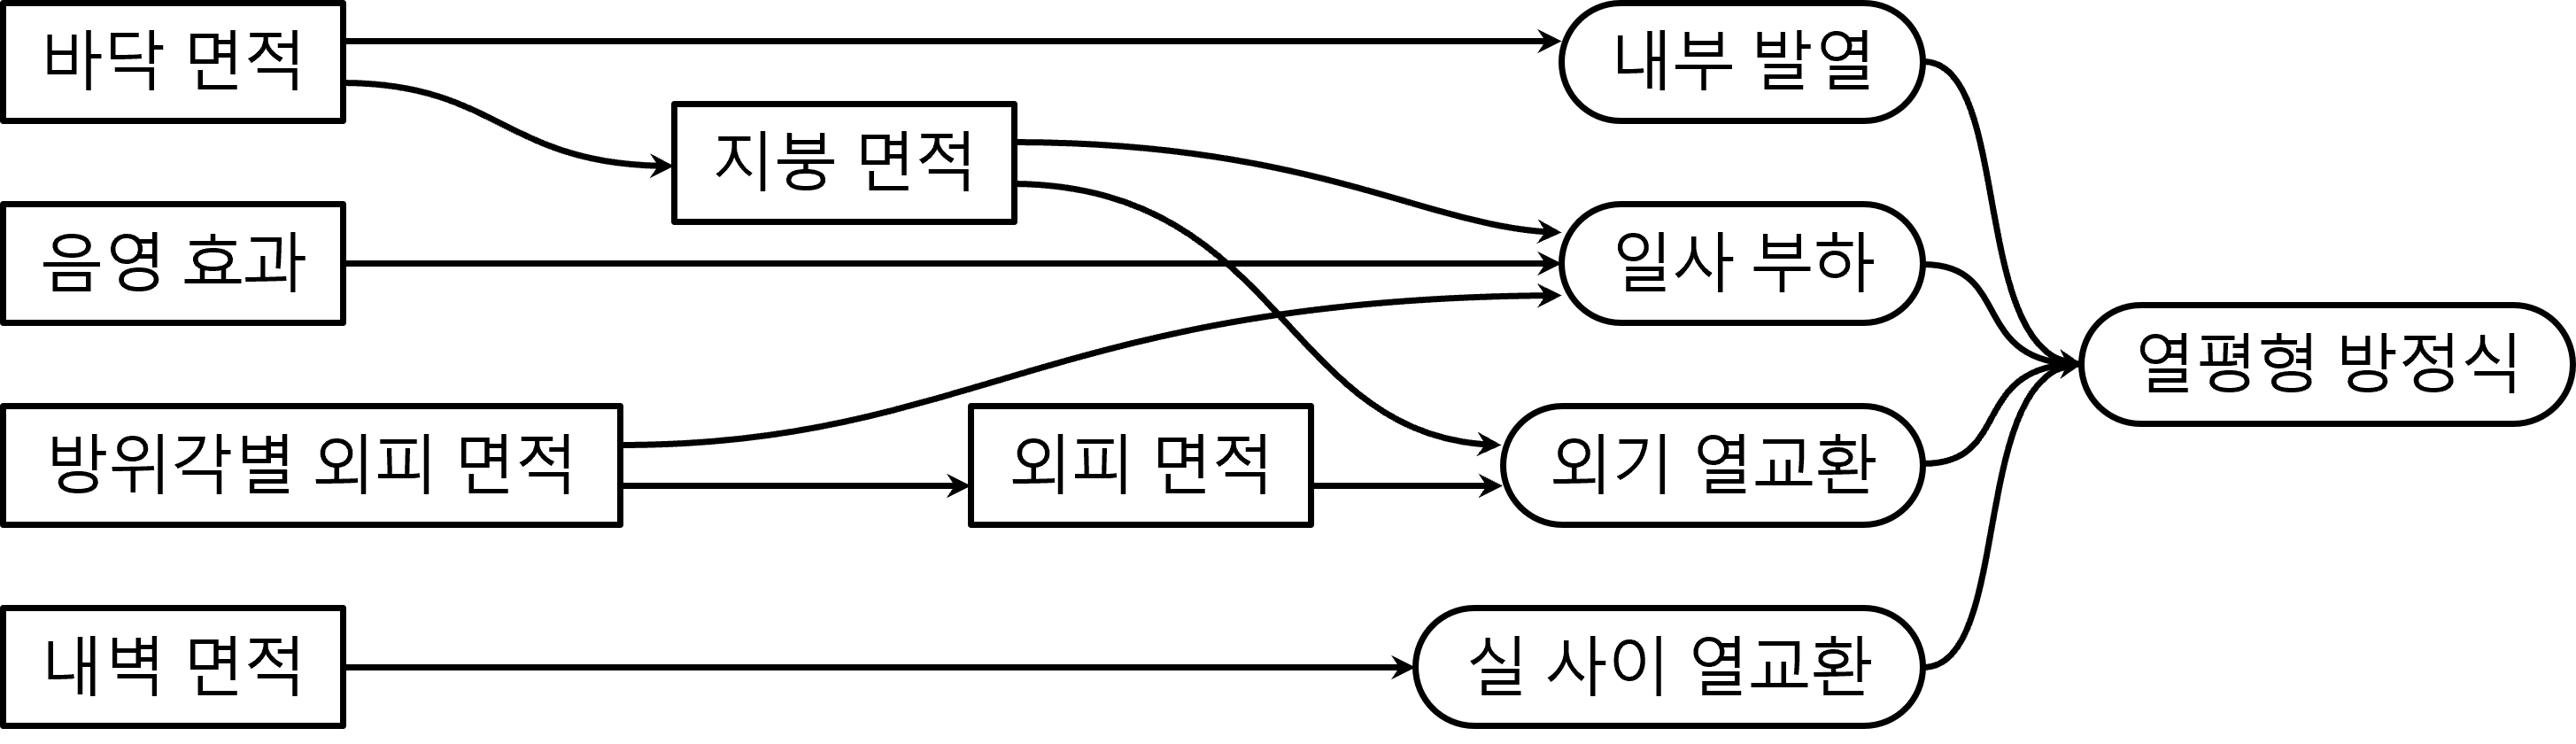
\includegraphics[width=0.8\textwidth]{geometry_mechanism2.png}
  \caption{열평형 방정식 도출 과정}
  \label{fig:geometry_mechanism2}
\end{defaultfigure}

\subsubsection{Detailed geometry, simplified geometry}

EnergyPlus의 형상 입력 방식은 크게 detailed geometry와 simplified geometry로 구분할 수 있다 (Figure \ref{fig:geometry_types}). Detailed geometry(DG)는 실제 실의 모양을 그대로 모델에 반영하는 방식으로, 면들을 구성하는 점들의 좌푯값을 상세하게 입력하게 된다. DesignBuilder, OpenStudio 등 일반적인 EnergyPlus 모델 저작 도구에서 사용하고 있다. 반면 simplified geometry(SG)는 실을 구성하는 각종 요소(벽, 바닥, 천장 등)와 동일한 면적과 방위각을 가지는 면들을 생성하여 열평형 방정식 계산에 사용하는 방식으로, 건물의 구체적인 형상이 구현되지 않아 건물 형상 및 차양을 직달 일사 계산에 반영하지 못한다는 특징이 있다. 이러한 한계에도 불구하고 비교적 간소화된 형상 입력만으로 상세한 동적 건물 에너지 시뮬레이션이 가능하다는 점에서 널리 사용되고 있으며, 미국 캘리포니아의 에너지 평가 툴인 CBECC (California's Building Energy Code Compliance Software)의 SG 방식\cite{cbecc}이 대표적인 예시이다. Simulator 역시 3D 모델링 프로그램 없이 비교적 간단한 입력을 통한 편의성 확보를 위해 SG 방식을 형상 입력 방식으로 체택하고 있다.

\begin{defaultfigure}
  
  \begin{subfigure}[b]{0.45\textwidth}
    \centering
    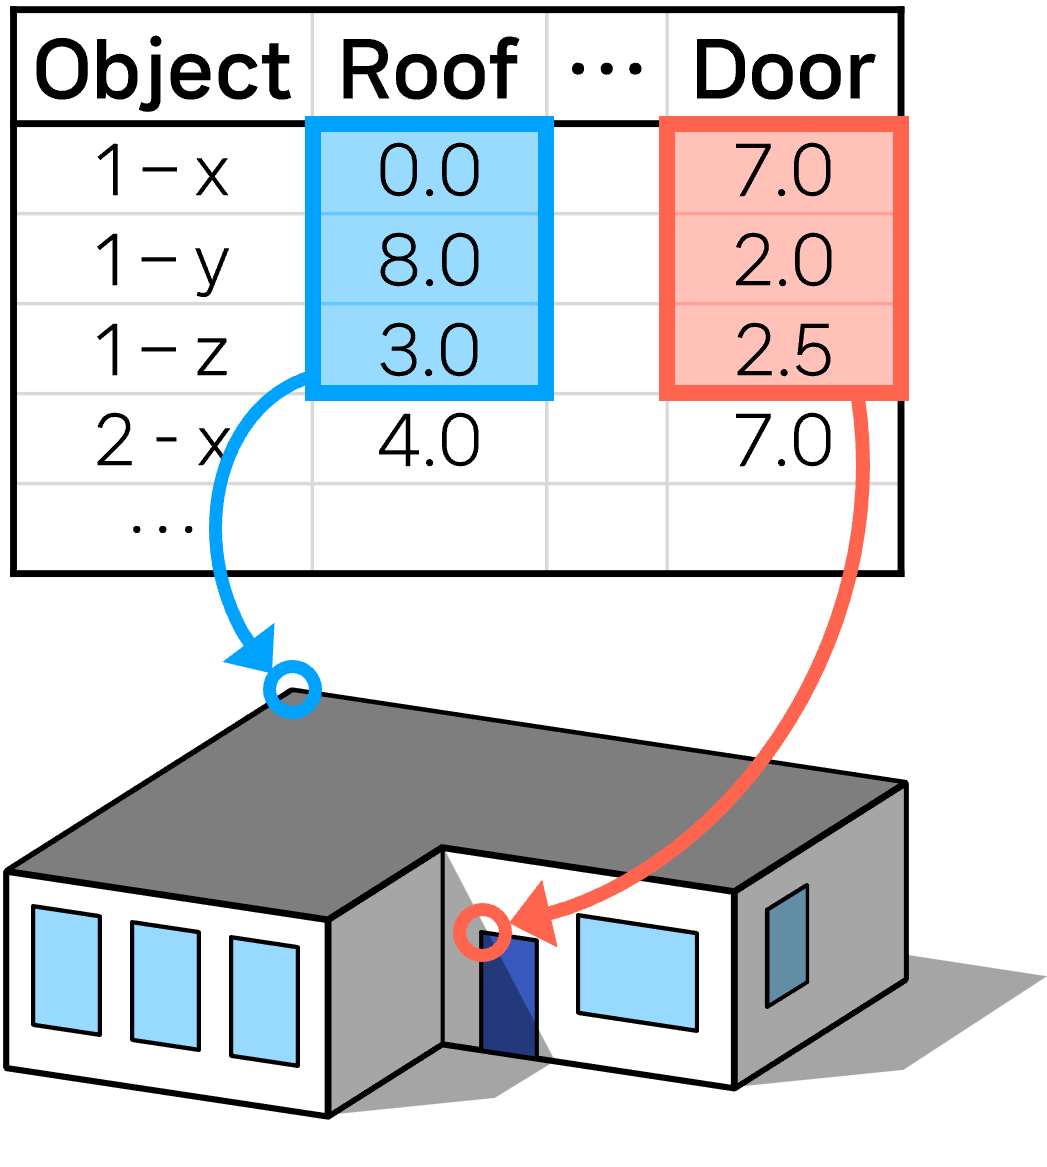
\includegraphics[scale=0.6]{형상_DG.png}
    \caption{detailed geometry}
  \end{subfigure}
  \hfill
  \begin{subfigure}[b]{0.45\textwidth}
    \centering
    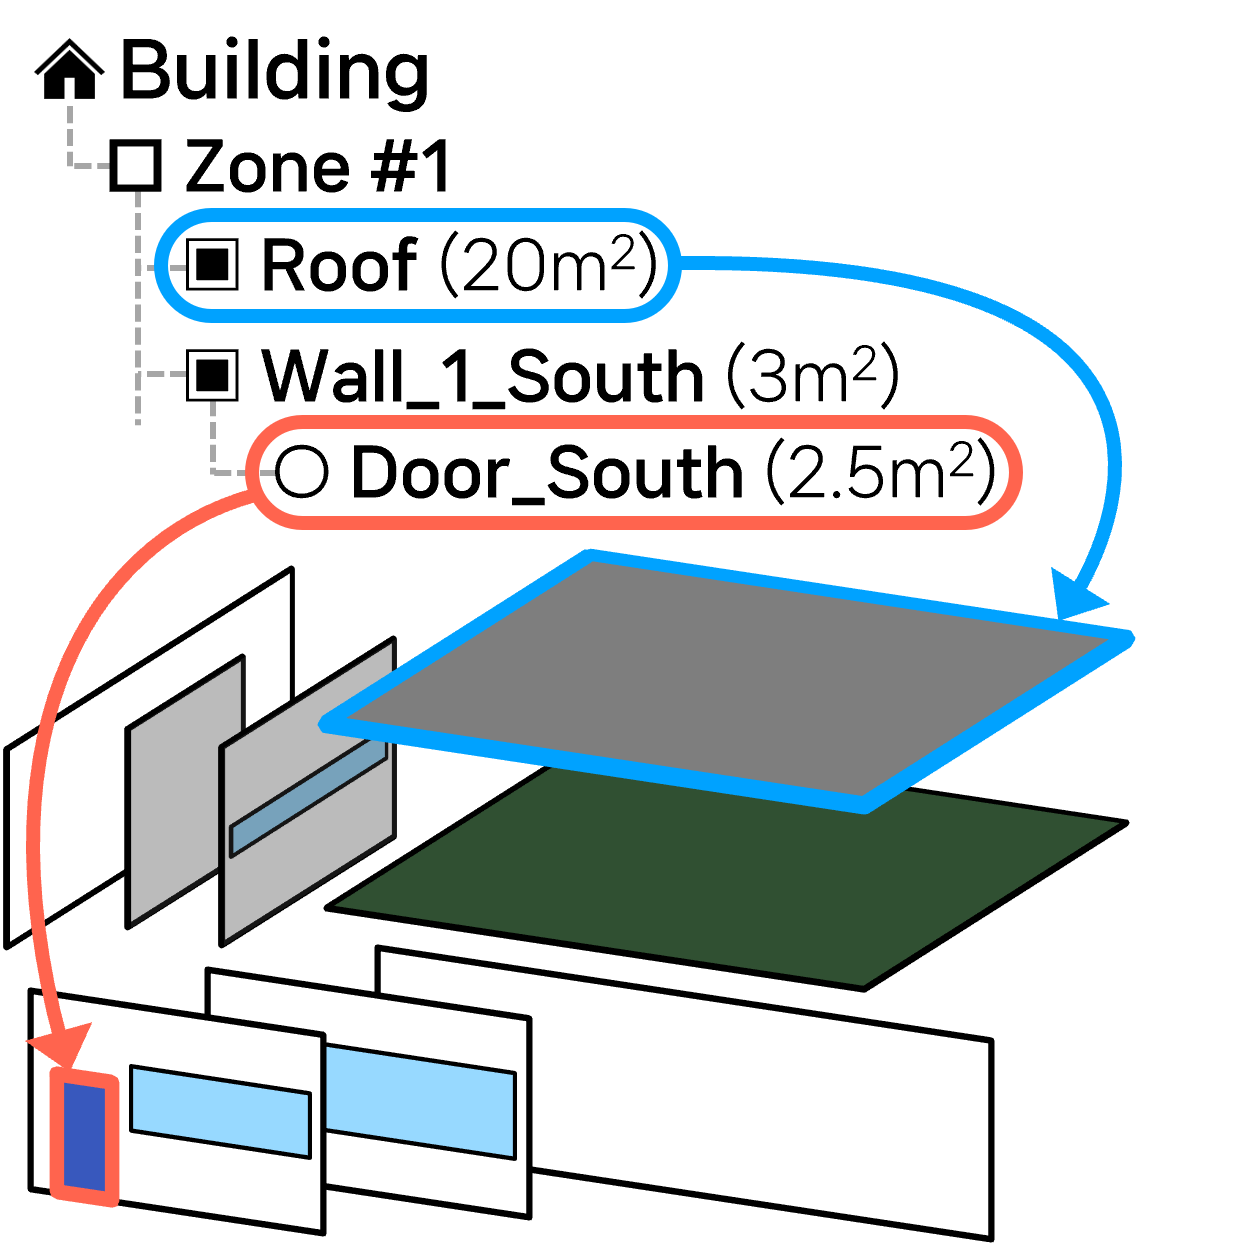
\includegraphics[scale=0.6]{형상_SG.png}
    \caption{simplified geometry}
  \end{subfigure}
  
  \caption{형상 입력 방식}
  \label{fig:geometry_types}

\end{defaultfigure}

\subsection{벽체, 지붕, 바닥 변환 방법}
Simplified Geometry를 \ep 입력 체계에 맞게 변환한다.

\subsubsection{좌표 생성}
천장은 높이 받아서 생성하고 나머지도 높이 받아서 만들고 바닥 만들고.
내벽의 경우 azimuth는 hash함수로 랜덤하게 생성한다. 

\subsubsection{clone 객체 생성}
copy한 벽체는 이를 azimuth를 180도 뒤집어주어야 한다.

\subsubsection{연산 옵션 설정}
EnergyPlus \texttt{Building} 객체의 \texttt{Solar Distribution} 속성을 `\texttt{MinimalShadowing}'으로 설정하며, 모든 \texttt{ShadowCalculation} 객체를 삭제한다.

\subsection{창호, 문 변환 방법}
벽의 일부로 직사각형을 생성한다. \ep의 ...객체를 이용한다.

\subsection{블라인드 변환 방법}
...

% ---------------------------------------------------------------------------- %
%                                  NEW SECTION                                 %
% ---------------------------------------------------------------------------- %

\section{구조체 정의}
\subsection{EnergyPlus 구조체의 정의 및 변환 방법}
EnergyPlus는 Material class에서 먼저 재료의 물성치 (열전도율, 밀도, 비열) 입력하고 구조체는 Construction class에서 하나씩 referecing해와서 구조체를 만드는 방식이다.
외부에서부터 내부 방향으로 각 layer가 어떻게 구성되어있는지 입력하는것이다.

\subsection{모르는 값 추정}
기축건물은 구조체를 모르는 경우가 많으며, 성적서 없는 경우도 다수 존재.
구조체 모르는 경우 법규 연계, 창호는 현장 조사에서 레이어 조사 후 DB에서 값 선택 등 @TODO
그린리모델링의 대상인 기축건물은 도면 및 시방서의 누락 등으로 인해 건물의 각 부위별 구조체를 모르는 경우가 많으며, 구조체 정보는 존재하더라도, 물성치에 대한 정보(시험성적서 등)가 없는 경우도 다수 존재한다. 이를 위해, 본 \simulator는 구조체를 모르는 경우 법규 연계, 창호는 현장 조사에서 레이어 조사 후 DB에서 값 선택 등 대안이 있다.


\subsubsection{재료}
ASHRAE 참고

\renewcommand{\arraystretch}{0.8}
\begin{longtable}{llcclc}
  \caption{기본 재료 물성치} \\
  \toprule
  재료명(국문) & \makecell{열전도도 \\ $[W{\cdot}m^{-1}{\cdot} K^{-1}]$}  & \makecell{밀도 \\ $[kg/m^{3}]$} & \makecell {비열 \\ $[J/kg\cdot K]$} & 재료명 (영문) &  출처 \\ \midrule
  \endfirsthead
  \multicolumn{6}{r}{\textit{(이전 페이지에서 계속)}} \\ \toprule
  재료명(국문) & \makecell{열전도도 \\ $[W{\cdot}m^{-1}{\cdot} K^{-1}]$}  & \makecell{밀도 \\ $[kg/m^{3}]$} & \makecell {비열 \\ $[J/kg\cdot K]$} & 재료명 (영문) & 출처 \\ \midrule
  \endhead
  \midrule \multicolumn{6}{r}{\textit{(다음 페이지에 계속)}} \\ \bottomrule
  \endfoot
  \bottomrule
  \endlastfoot
  시멘트벽돌 &   0.600 &  464 & 0.88 & LW concrete block & \cite{ashrae_f18} \\
  내화벽돌 &   0.990 & 1920 & 0.79 & brick & \cite{ashrae_f18} \\
  타일 &   1.300 & 1920 & 1.26 & Slate or tile & \cite{ashrae_f18} \\
  콘크리트블록(경량) &   0.700 &  512 & 0.88 & LW concrete block & \cite{ashrae_f18} \\
  콘크리트블록(중량) &   1.000 &  800 & 0.92 & concrete block & \cite{ashrae_f18} \\
  대리석 &   2.800 & 2560 & 0.79 & stone & \cite{ashrae_f18} \\
  화강암 &   3.300 & 2560 & 0.79 & stone & \cite{ashrae_f18} \\
  천연슬레이트 &   1.500 & 1920 & 1.26 & Slate or tile & \cite{ashrae_f18} \\
  파티클보드 &   0.150 &  400 & 1.30 & fiberboard sheathing & \cite{ashrae_f18} \\
  석고보드 &   0.180 &  800 & 1.09 & gyp board & \cite{ashrae_f18} \\
  목재(가벼움) &   0.140 &  608 & 1.63 & wood & \cite{ashrae_f18} \\
  목재(중간) &   0.170 &  608 & 1.63 & wood & \cite{ashrae_f18} \\
  목재(무거움) &   0.190 &  608 & 1.63 & wood & \cite{ashrae_f18} \\
  바닥재(아스팔트) &   0.330 & 1120 & 1.26 & Asphalt shingles & \cite{ashrae_f18} \\
  아스팔트펠트17kg &   0.110 & 1120 & 1.26 & Asphalt shingles & \cite{ashrae_f18} \\
  아스팔트펠트22kg &   0.140 & 1120 & 1.26 & Asphalt shingles & \cite{ashrae_f18} \\
  아스팔트펠트26kg &   0.220 & 1120 & 1.26 & Asphalt shingles & \cite{ashrae_f18} \\
  아스팔트루핑17kg &   0.190 & 1120 & 1.46 & Built-up roofing & \cite{ashrae_f18} \\
  아스팔트루핑22kg &   0.270 & 1120 & 1.46 & Built-up roofing & \cite{ashrae_f18} \\
  아스팔트루핑30kg &   0.340 & 1120 & 1.46 & Built-up roofing & \cite{ashrae_f18} \\
  콘크리트(1:2:4) &   1.600 & 2240 & 0.90 & heavyweight concrete & \cite{ashrae_f18} \\
  기포콘크리트0.4품 &   0.130 & 1280 & 0.84 & lightweight concrete & \cite{ashrae_f18} \\
  기포콘크리트0.5품 &   0.160 & 1280 & 0.84 & lightweight concrete & \cite{ashrae_f18} \\
  기포콘크리트0.6품 &   0.190 & 1280 & 0.84 & lightweight concrete & \cite{ashrae_f18} \\
  비드법보온판1종1호 &   0.036 &   43 & 1.21 & insulation board & \cite{ashrae_f18} \\
  비드법보온판1종2호 &   0.037 &   43 & 1.21 & insulation board & \cite{ashrae_f18} \\
  비드법보온판1종3호 &   0.040 &   43 & 1.21 & insulation board & \cite{ashrae_f18} \\
  비드법보온판1종4호 &   0.043 &   43 & 1.21 & insulation board & \cite{ashrae_f18} \\
  비드법보온판2종1호 &   0.031 &   43 & 1.21 & insulation board & \cite{ashrae_f18} \\
  비드법보온판2종2호 &   0.032 &   43 & 1.21 & insulation board & \cite{ashrae_f18} \\
  비드법보온판2종3호 &   0.033 &   43 & 1.21 & insulation board & \cite{ashrae_f18} \\
  비드법보온판2종4호 &   0.034 &   43 & 1.21 & insulation board & \cite{ashrae_f18} \\
  압출법보온판특호 &   0.027 &   43 & 1.21 & insulation board & \cite{ashrae_f18} \\
  압출법보온판1호 &   0.028 &   43 & 1.21 & insulation board & \cite{ashrae_f18} \\
  압출법보온판2호 &   0.029 &   43 & 1.21 & insulation board & \cite{ashrae_f18} \\
  압출법보온판3호 &   0.031 &   43 & 1.21 & insulation board & \cite{ashrae_f18} \\
  경질우레탄보온판1종1호 &   0.024 &   43 & 1.21 & insulation board & \cite{ashrae_f18} \\
  경질우레탄보온판1종2호 &   0.024 &   43 & 1.21 & insulation board & \cite{ashrae_f18} \\
  경질우레탄보온판1종3호 &   0.025 &   43 & 1.21 & insulation board & \cite{ashrae_f18} \\
  경질우레탄보온판2종1호 &   0.023 &   43 & 1.21 & insulation board & \cite{ashrae_f18} \\
  경질우레탄보온판2종2호 &   0.023 &   43 & 1.21 & insulation board & \cite{ashrae_f18} \\
  경질우레탄보온판2종3호 &   0.024 &   43 & 1.21 & insulation board & \cite{ashrae_f18} \\
  미네랄울보온판1호 &   0.037 &   19 & 0.96 & batt insulation & \cite{ashrae_f18} \\
  미네랄울보온판2호 &   0.036 &   19 & 0.96 & batt insulation & \cite{ashrae_f18} \\
  미네랄울보온판3호 &   0.038 &   19 & 0.96 & batt insulation & \cite{ashrae_f18} \\
  미네랄울펠트 &   0.039 &   19 & 0.96 & batt insulation & \cite{ashrae_f18} \\
  미네랄울보온대1호 &   0.040 &   19 & 0.96 & batt insulation & \cite{ashrae_f18} \\
  미네랄울보온대2호 &   0.039 &   19 & 0.96 & batt insulation & \cite{ashrae_f18} \\
  미네랄울보온통 &   0.036 &   19 & 0.96 & batt insulation & \cite{ashrae_f18} \\
  그라스울보온판24K &   0.037 &   19 & 0.96 & batt insulation & \cite{ashrae_f18} \\
  그라스울보온판32K &   0.036 &   19 & 0.96 & batt insulation & \cite{ashrae_f18} \\
  그라스울보온판40K &   0.035 &   19 & 0.96 & batt insulation & \cite{ashrae_f18} \\
  그라스울보온판48K-120K &   0.034 &   19 & 0.96 & batt insulation & \cite{ashrae_f18} \\
  그라스울보온통 &   0.036 &   19 & 0.96 & batt insulation & \cite{ashrae_f18} \\
  미네랄울 &   0.044 &   19 & 0.96 & batt insulation & \cite{ashrae_f18} \\
  미네랄울블랭킷1호a &   0.039 &   19 & 0.96 & batt insulation & \cite{ashrae_f18} \\
  미네랄울블랭킷1호b &   0.037 &   19 & 0.96 & batt insulation & \cite{ashrae_f18} \\
  미네랄울블랭킷2호 &   0.036 &   19 & 0.96 & batt insulation & \cite{ashrae_f18} \\
  그라스울 &   0.035 &   19 & 0.96 & batt insulation & \cite{ashrae_f18} \\
  그라스울보온대a &   0.044 &   19 & 0.96 & batt insulation & \cite{ashrae_f18} \\
  그라스울보온대b &   0.044 &   19 & 0.96 & batt insulation & \cite{ashrae_f18} \\
  그라스울보온대c &   0.044 &   19 & 0.96 & batt insulation & \cite{ashrae_f18} \\
  그라스울블랭킷a &   0.040 &   19 & 0.96 & batt insulation & \cite{ashrae_f18} \\
  그라스울블랭킷b &   0.036 &   19 & 0.96 & batt insulation & \cite{ashrae_f18} \\
  동 & 370 & 7824 & 0.50 & Metal surface & \cite{ashrae_f18} \\
  청동(75Cu,25Sn) &  25 & 7824 & 0.50 & Metal surface & \cite{ashrae_f18} \\
  황동(70CU,30Zn) & 110 & 7824 & 0.50 & Metal surface & \cite{ashrae_f18} \\
  알루미늄/합금 & 200 & 7824 & 0.50 & Metal surface & \cite{ashrae_f18} \\
  강재 &  53 & 7824 & 0.50 & Metal surface & \cite{ashrae_f18} \\
  납 &  34 & 7824 & 0.50 & Metal surface & \cite{ashrae_f18} \\
  아연도철판 &  44 & 7824 & 0.50 & Metal surface & \cite{ashrae_f18} \\
  스텐레스강 &  15 & 7824 & 0.50 & Metal surface & \cite{ashrae_f18} \\
  \bottomrule
\end{longtable}

\subsubsection{구조체}
구조체와 실내외 표면열전달저항 값은 에너지절약설계기준값을 참고하였다. 임의의 구조체는 콘크리트와 단열재 레이어를 이용하여 정의한다 (아래 RC diagram 그림).\par
참고로 EnergyPlus에서는 실내외 표면열전달저항 동적으로 계산된다. 수식은 아래와 같고, 시뮬레이션 해보니 보통 아래와 같다. 
\begin{tcolorbox}[colback=gray!10, colframe=gray!80, boxrule=0.5pt, left=1em, right=1em]
1년간 hout hin 변화하는 그림 (에절서에 정의된 값이랑 비교)
\end{tcolorbox}

\subsubsection{창호}
창호는 법규에서 U값은 지정하고 있으나 SHGC는 따로 규정한 바 없으며, 현장에서 알 수가 없는 경우가 많다. 
창호 종류에 따라 U, SHGC값을 선택하도록 만들었으며, 이 선택은 에너지절약설계기준을 참고하였다. 참고로, 에절서에 있는 창호 종류별 성능은 에절서 제정된 2013년 이후로 개정된 바 없다.


% ---------------------------------------------------------------------------- %
%                                  NEW SECTION                                 %
% ---------------------------------------------------------------------------- %

\section{프로필 정의와 활용}
\subsection{ECO2 프로필의 정의}
건축물에너지효율등급인증규정은 건물 에너지 모델 구축 과정에서 실의 용도를 프로필로 지정하도록 하고 있으며, 총 23개의 프로필을 제공한다\cite{law:usageprofile}. 국내 용도프로필은 (1)사용시간과 운전 시간, (2)설정 요구량, (3)열발열원, (4)실내공기온도, (5)월간 사용일수에 관한 정보를 담고 있다 (\cref{tab:smallofficeusage}). 

\begin{table}[ht]
  \caption{ECO2:주거 및 주거용 이외 건축물 용도프로필 종류}
  \label{tbl:eco2profiles}  
  \centering
  \begin{tabular}{llll}
    \toprule
    번호 & 프로필명 & 번호 & 프로필명 \\ \midrule
    (1) & 주거공간             & (11) & 전산실 \\ \midrule
    (2) & 소규모사무실(30m2이하) & (12) & 주방 및 조리실 \\ \midrule
    (3) & 대규모사무실(30m2초과) & (13) & 병실 \\ \midrule
    (4) & 회의실 및 세미나실     & (14) & 객실 \\ \midrule
    (5) & 강당                & (15) & 교실(초중고) \\ \midrule
    (6) & 구내식당             & (16) & 강의실(대학) \\ \midrule
    (7) & 화장실               & (17) & 매장(상점/백화점) \\ \midrule
    (8) & 그 외 체류공간 (휴게실, 탈의실, 헬스장, 등) & (18) & 전시실(전시관/박물관) \\ \midrule
    (9) & 부속공간 (로비, 복도, 계단실 등) & (19) & 열람실(도서관) \\ \midrule
    (10) & 창고/설비/문서실     & (20) & 체육시설 \\ \bottomrule
  \end{tabular}
\end{table}



\renewcommand{\arraystretch}{0.85}
\begin{longtable}{ccc}
  \caption{용도프로필 입력값 예시: 소규모사무실($30m^2$이하)} \\
  \label{tab:smallofficeusage} \\
  \toprule
  구분 & 단위 & 값 \\ \midrule
  \endfirsthead
  \multicolumn{3}{r}{\textit{(이전 페이지에서 계속)}} \\ \toprule
  구분 & 단위 & 값 \\ \midrule
  \endhead
  \midrule \multicolumn{3}{r}{\textit{(다음 페이지에 계속)}} \\ \bottomrule
  \endfoot
  \bottomrule
  \endlastfoot
  % 본문 데이터 (예시)
  사용시간과 운전시간 & & \\
  \midrule
  사용시작시간 & [hh:mm] & 09:00 \\
  사용종료시간 & [hh:mm] & 18:00 \\
  운전시작시간 & [hh:mm] & 07:00 \\
  운전종료시간 & [hh:mm] & 18:00 \\
  \midrule
  설정 요구량 & & \\
  \midrule
  최소도입외기량 & [$m^3/(m^2h)$] & 4 \\
  급탕요구량 & [$Wh/(m^2d)$] & 30 \\
  조명시간 & [h] & 6 \\
  \midrule
  열발열원 & & \\
  \midrule
  사람 & [$Wh/(m^2d)$] & 30 \\
  작업보조기기 & [$Wh/(m^2d)$] & 42 \\
  \midrule
  실내공기온도 & & \\
  \midrule
  난방설정온도 & [°C] & 20 \\
  냉방설정온도 & [°C] & 26 \\
  \midrule
  월간 사용일수 & & \\
  \midrule
  1월 사용일수 & [d/mth] & 22 \\
  2월 사용일수 & [d/mth] & 19 \\
  3월 사용일수 & [d/mth] & 21 \\
  4월 사용일수 & [d/mth] & 22 \\  
  5월 사용일수 & [d/mth] & 22 \\
  6월 사용일수 & [d/mth] & 20 \\
  7월 사용일수 & [d/mth] & 22 \\
  8월 사용일수 & [d/mth] & 21 \\
  9월 사용일수 & [d/mth] & 18 \\
  10월 사용일수 & [d/mth] & 21 \\
  11월 사용일수 & [d/mth] & 21 \\
  12월 사용일수 & [d/mth] & 21 \\
\end{longtable}



\subsection{EnergyPlus 프로필의 정의}
본 시뮬레이터는 EnergyPlus의 \texttt{Schedule:Compact}를 활용하여 용도프로필의 값을 적용하며, \cref{fig:ep_profile_structure}\와 같은 구조로 구성한다.

\begin{itemize}
  \item \textbf{Level 1(일간스케줄)}: 하루를 10분 간격으로 나누고, 각 간격에 해당하는 값을 순서대로 나열하여 구성한다. (예: 10분 간격일 경우 144개(1일;24시간;1440분)의 값으로 입력한다)
  \item \textbf{Level 2(스케줄규칙)}: Level 1에서 정의한 일간스케줄을 요일(예: 주중, 주말, 공휴일 등) 유형에 따라 규칙을 정의한다. 즉, 어떤 요일 유형에 어떤 일간스케줄을 적용할지 결정한다. 예를 들어, \cref{fig:ep_profile_structure}의 ``주중 9to6 yes/no"스케줄의 경우, 9to6 yes/no(기본)을 모든 요일의 기본스케줄로 설정하되, 주말(토/일)과 휴일(공휴일)은 ``하루종일 no"스케줄을 override한다.
  \item \textbf{Level 3(연간스케줄)}: 1년 동안의 스케줄을 정의한다. Level 2의 스케줄 규칙을 특정 기간에 맞게 조합하여 연간스케줄을 구성한다. 이를 통해, 방학 등 특정 기간에 따른 스케줄 변화가 필요한 실의 스케줄을 입력한다.
  \item \textbf{Level 4(프로필)}: 실 운영관련 인자(기기가동, 재실, 조명, 실내 설정온도)의 연간스케줄(Level 3)최종 스케줄 객체이다.
\end{itemize}

이처럼, EnergyPlus 스케줄은 일간스케줄(Level 1) $\to$ 스케줄규칙(Level 2) $\to$ 연간스케줄(Level 3) $\to$ 프로필(Level 4)순서로 조합되어, 실 용도별 운영 스케줄을 상세하게 반영할 수 있도록 지원한다.

\begin{defaultfigure}
  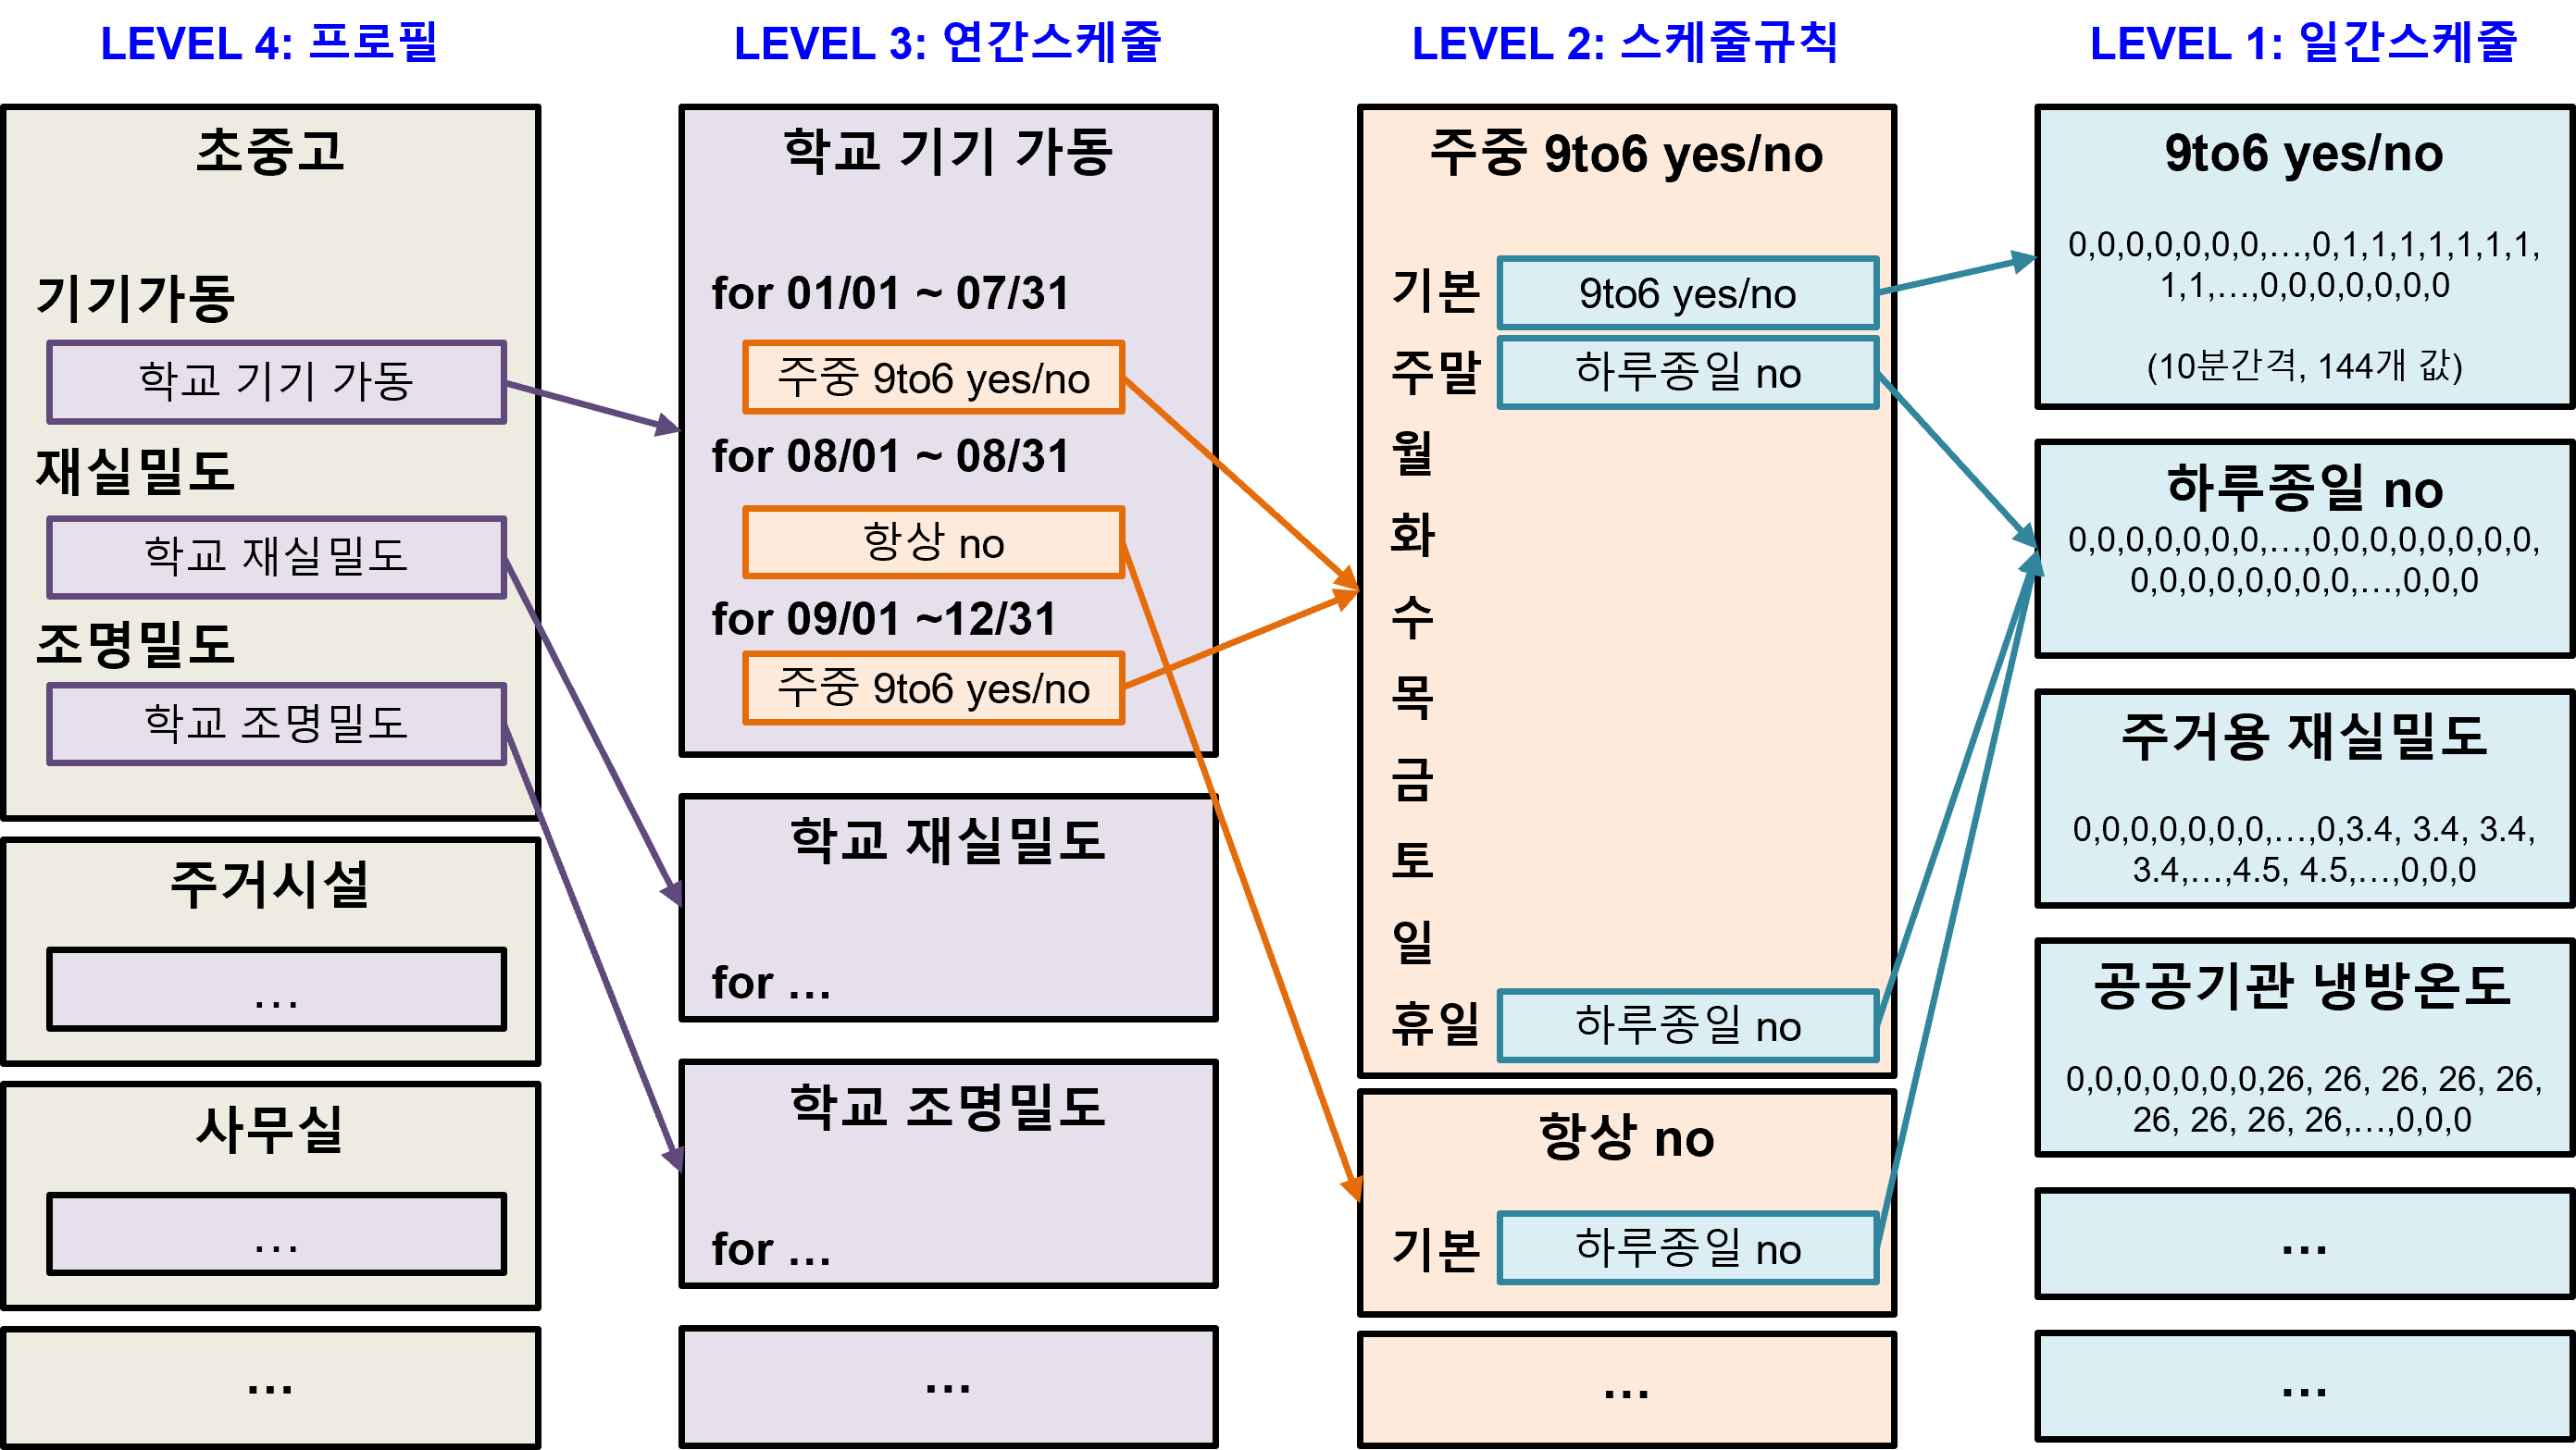
\includegraphics[width=\textwidth]{프로필구조도.png}
  \caption{EP 프로필 구조 예시}
  \label{fig:ep_profile_structure}
\end{defaultfigure}

\subsection{건축물에너지효율등급인증규정의 용도프로필을 EnergyPlus 프로필로 변환 방법}
현재 건축물에너지효율등급인증규정에서 사용하는 용도프로필은 각 항목의 "대표값"으로 단순하게 구성되어있다. 이를 EnergyPlus에서 활용하기 위해서는, 두 가지 핵심 변환 과정이 요구된다.

\begin{enumerate}
  \item 단위 및 값 변환: 건축물에너지효율등급인증규정의 용도프로필의 값(예:열발열원-사람 [$Wh/(m^2d)$])을 EnergyPlus가 요구하는 단위 (예:면적당 인원 [$people/m^2$])로 변환한다.
  \item 스케줄 변환: 건축물에너지효율등급인증규정의 단순 운영 시간 및 운영일수를 EnergyPlus 스케줄 형식으로 변환한다.
\end{enumerate}

아래는 건축물에너지효율등급인증규정의 소규모 사무소(30$m^2$이하)(\cref{tab:smallofficeusage})의 프로필을 EnergyPlus입력 스케줄로 변환하는 과정의 예시이다.

\subsubsection{재실밀도}
\begin{table}[ht]
  \caption{재실스케줄 변환}
  \centering
  \begin{tabular}{lcc}
    \toprule
     & \makecell{에너지효율등급\\인증규정} & EnergyPlus\\ \midrule
    재실밀도 &  30 [$Wh/(m^2d)$] & 0.048 [$people/m^2$] \\ \midrule
    스케줄  &  09:00-18:00      & \makecell{주중 09:00-18:00\\ 주말 및 공휴일 0} \\ \midrule
  \end{tabular}
\end{table}

\paragraph{단위 및 값 변환} 건축물에너지효율등급인증규정은 인체의 발열량을 일일 면적당 발열 [$Wh/(m^2d)$]로 정의한다. 반면, EnergyPlus는 인체의 발열을 (a)인당 발열량 [$W/person$]과 (b) 단위 면적당 재실 인원 [$people/m^2$]의 조합으로 입력한다. 본 시뮬레이터에서는 인체의 현열 발열량을 70 [$W/person$]으로 가정하여 변환하였다.\par
  (30$Wh/(m^2d)$ $\div$ 사용시간 9h $\div$ 인체발열(현열) 70 W/person = 0.048 $people/m^2$)
\paragraph{스케줄 변환} 인증규정에 명시된 사용시간(09:00-18:00)과 월간 사용일수를 바탕으로 EnergyPlus의 연간 스케줄을 생성한다. 사용시간은 주중(Weekdays)스케줄에 적용하며, 주말(Weekends) 및 공휴일(Holidays)에는 재실이 없는 것으로 설정한다.


\subsubsection{조명}
\begin{table}[ht]
  \caption{조명스케줄 변환}
  \centering
  \begin{tabular}{lcc}
    \toprule
     & \makecell{에너지효율등급\\인증규정} & EnergyPlus \\ \midrule
    스케줄  &  6 [h]      & \makecell{주중 10:00-11:00,13:00-18:00(6[h])\\ 주말 및 공휴일 0} \\ \midrule
  \end{tabular}
\end{table}

\paragraph{스케줄 변환} 인증규정의 일일 조명시간 6시간을 충족하기 위해, 점심시간을 제외한 주 업무시간대를 반영하여 EnergyPlus스케줄을 10-11시 및 13-18시로 설정하였다.



\subsubsection{작업보조기기 발열}
\begin{table}[ht]
  \caption{작업보조기기스케줄 변환}
  \centering
  \begin{tabular}{lcc}
    \toprule
     & \makecell{에너지효율등급\\인증규정} & EnergyPlus \\ \midrule
    기기발열 &  42 [$Wh/(m^2d)$] & 4.7 [$W/m^2$]  \\ \midrule
    스케줄  &  09:00-18:00      & \makecell{주중 09:00-18:00\\ 주말 및 공휴일 0} \\ \midrule
  \end{tabular}
\end{table}

\paragraph{단위 및 값 변환} 건축물에너지효율등급인증규정은 작업보조기기의 발열량을 일일 면적당 발열 [$Wh/(m^2d)$]의 단위로 정의한다. 반면, EnergyPlus는 작업보조기기의 발열을 면적당 발열량 [$W/m^2$]로 입력한다.\par
  (42$Wh/(m^2d)$ $\div$ 사용시간 9h = 4.7 $W/m^2$)
\paragraph{스케줄 변환} 재실스케줄과 같게 설정한다.



\subsubsection{최소도입외기량}
\begin{table}[ht]
  \caption{최소도입외기량 변환}
  \centering
  \begin{tabular}{lcc}
    \toprule
     & \makecell{에너지효율등급\\인증규정} & EnergyPlus\\ \midrule
    최소도입외기량 &  4 [$m^3/(m^2{\cdot}h)$] & 0.0011 [$m^3/(m^2{\cdot}s)$]  \\ \midrule
    스케줄  &  09:00-18:00      & \makecell{주중 09:00-18:00\\ 주말 및 공휴일 0}  \\ \midrule
  \end{tabular}
\end{table}


\paragraph{단위 및 값 변환} 건축물에너지효율등급인증규정은 최소도입외기량을 시간-단위면적당 외기도입량[$m^3/(m^2{\cdot}h)$]으로 정의한다. 반면, EnergyPlus는 최소도입외기량을 초-단위면적당 외기도입량[$m^3/(m^2{\cdot}s)$]으로 정의한다.\par
  (4 $m^3/(m^2{\cdot}h)$ $\div$ 3600 s = 0.0011 $m^3/(m^2{\cdot}s)$)
\paragraph{스케줄 변환} 재실스케줄과 같게 설정한다.


\subsubsection{냉난방 가동 및 설정온도}
\begin{table}[ht]
  \caption{냉난방 가동 및 설정온도 변환}
  \centering
  \begin{tabular}{lcc}
    \toprule
     & \makecell{에너지효율등급\\인증규정} & EnergyPlus\\ \midrule
    난방설정온도 &  20 [°C] & 20 [°C] \\ \midrule
    냉방설정온도 &  26 [°C] & 26 [°C] \\ \midrule
    스케줄      &  07:00-18:00   & \makecell{주중 07:00-18:00\\ 주말 및 공휴일 0}  \\ \midrule
  \end{tabular}
\end{table}

\paragraph{단위 및 값 변환} 에너지효율등급규정의 값을 동일하게 적용한다.
\paragraph{스케줄 변환} 인증규정에 명시된 운전시간(07:00-18:00)과 월간 사용일수를 바탕으로 EnergyPlus의 연간 스케줄을 생성한다. 운전시간은 주중(Weekdays)스케줄에 적용하며, 주말(Weekends) 및 공휴일(Holidays)에는 설비를 운전하지 않는 것으로 설정한다.


% ---------------------------------------------------------------------------- %
%                                  NEW SECTION                                 %
% ---------------------------------------------------------------------------- %

\section{설비 변환 알고리즘}
\subsection{Simulator 설비 데이터의 구조와 이해}
공급-생산 이원화하였다.

\subsection{EnergyPlus 설비 데이터의 구조와 이해}
branch와 loop 개념을 사용한다. supply와 demand로 구분되어있다.

\subsection{공급 및 생산 설비 변환 방법}
\subsubsection{데이터 구조 변환}
생산설비로 supply loop와 demand loop 일부를 만들고, 공급설비에서 demand branch를 만든다.
branchlist등 후처리한다.

\subsubsection{모르른 변수 추정}

ASHRAE 등 참고하는 것을 기본으로 한다.

각 설비시스템 별 사용자 입력변수, 시뮬레이터가 가정하는 변수, \ep가 기본적으로 제공하는 변수들은 아래 그림들과 같다.

\subsection{전열교환기 변환 방법}
ventilation에 포함된다.

\subsection{태양광패널 변환 방법}
가상의 surface를 생성하고, ...

% ---------------------------------------------------------------------------- %
%                                  NEW SECTION                                 %
% ---------------------------------------------------------------------------- %

\chapter{시뮬레이션 결과의 해석}

\section{EnergyPlus의 실행 결과물 종류와 의미}
연료별 table 생성하고 읽어들인다.

\subsection{EP 결과 내는 법과 의미}
Table:Output 활용한다. Output은 6가지로 구분되는데, heating, cooling, lighting, fan, pump, cogeneration, ...

\subsubsection{heating}
heating에는 ... 에서 소요되는 에너지가 포함된다.

\subsubsection{cooling}
cooling에는 ... 에서 소요되는 에너지가 포함된다.

\subsubsection{lighting}
lighting에는 ... 에서 소요되는 에너지가 포함된다.

\subsubsection{fan}
fan에는 ... 에서 소요되는 에너지가 포함된다.
예를들어, 전열교환기를 설치하는 경우 전열교환기 팬이 사용하는 전력은 여기에 들어간다.

\subsubsection{pump}
pump에는 ... 에서 소요되는 에너지가 포함된다. ...설비들을 모델링하면 펌프가 자동으로 생성되어 에너지사용량에 포함된다.

\subsubsection{cogeneration}
PV패널 발전량이다.

\subsection{EP 결과 읽는 법과 의미}
냉방, 난방, 조명, 팬/펌프/전열교환기, 급탕, 발전은,
각각 heating, cooling, lighting, fan과 pump, domestic hot water, cogeneration에 대응된다.

% ---------------------------------------------------------------------------- %
%                                  NEW SECTION                                 %
% ---------------------------------------------------------------------------- %

\section{그린리모델링을 위한 결과 해석}

\subsection{단위면적당 에너지소비량} \label{subsec:floorarea_definition_for_EUI}
가장 널리 사용되는 단위면적당 에너지 소요량 (EUI) 씀. 여기서 단위면적당에는 ...까지 포함된다. 바닥면적은 공조하는 모든 zone의 바닥면적의 총합이다.

\subsection{산출 지표들} \label{subsec:result_converting_coeff_definition}
\simulator\은 계산된 용도별, 열원별, 월별 에너지소요량을 바탕으로, 1차에너지소요량, 온실가스 배출량 및 에너지 비용을 산출하여 제시한다. 각 지표에 대한 변환 계수는 본 엔진에서 지원하는 4가지 연료(전기, 천연가스, 등유, 지역난방)에 대하여 각각 정의되며, 건물 전체의 1차에너지소요량, 온실가스배출량 및 에너지 비용은 4가지 연료에 대한 값의 합으로 정의된다 (식 \ref{eq:1st_energy_calculation} - \ref{eq:cost_calculation}).

\begin{align}
  \text{건물 전체의 에너지소요량} = \sum_{\text{연료}} \text{연료별 에너지소요량} \times \text{연료별 변환계수} \label{eq:1st_energy_calculation}\\
  \text{건물 전체의 온실가스 배출량} = \sum_{\text{연료}} \text{연료별 에너지소요량} \times \text{연료별 변환계수} \label{eq:co2_calculation}\\ 
  \text{건물 전체의 에너지 비용} = \sum_{\text{연료}} \text{연료별 에너지소요량} \times \text{연료별 변환계수} \label{eq:cost_calculation}
\end{align}

\subsubsection{1차에너지소요량}
연료별 1차에너지 환산 계수는 표 \ref{tbl:coeff_kWh_to_1stkWh}\와 같다. 이는 제로에너지건축물 인증제도 운영규정 \cite{law:energy_to_1stenergy} 에서 제시하고 있다. 국내에서는 모든 연료에 대하여 대표적인 환산계수만을 제시하고 있어 \cite{Jeong2021energydeungkeup}, 가스 및 등유에 대하여 동일한 환산계수를 적용하였다.

\begin{table}[ht]
  \caption{연료별 사용량의 1차에너지 환산 계수}
  \label{tbl:coeff_kWh_to_1stkWh}  
  \centering
  \begin{tabular}{cr}
    \toprule
    연료명 & \makecell{환산계수 \\ $[kWh/kWh]$} \\ \midrule
    전기 & 2.75 \\
    가스 & 1.1 \\
    등유 & 1.1 \\
    지역난방 & 0.728 \\ \bottomrule
  \end{tabular}
\end{table}

1차에너지 환산계수는 관련 법령의 개정에 따라 수정 반영되어야 한다.

\subsubsection{온실가스 배출량}
연료별 온실가스 배출량 환산 계수는 표 \ref{tbl:coeff_kWh_to_CO2}\와 같다. 온실가스는 CO\textsubscript{2,eq}로 계산하는게 표준임. eq 계산은 어떻게 함. 온실가스 종류별 CO2변환계수(지구온난화지수?)는 아래 표 참고 바람.

\begin{table}[ht]
  \caption{연료별 사용량의 온실가스 배출량 환산 계수}
  \label{tbl:coeff_kWh_to_CO2}  
  \centering
  \begin{tabular}{cr}
    \toprule
    연료명 & 환산계수 [kgCO\textsubscript{2,eq}/kWh] \\ \midrule
    전기 & 0.4541 \\
    가스 & 0.2024 \\
    등유 & 0.2603 \\
    지역난방 & 0.1358 \\ \bottomrule
  \end{tabular}
\end{table}

\paragraph{전기} 전기의 온실가스 배출량 환산 계수는 매년 환경부 온실가스 종합정보센터에서 공포하고 있다.
\paragraph{가스 및 등유} 이건 좀 복잡한데, IPCC에서... 이런 수식을 사용하고 있고, 이런 표를 제시하고 있고, 그 값은 아래 표와 같고...

\paragraph{지역난방} 지역난방의 온실가스 배출량 환산 계수는 매년 3월 경 한국지역난방공사에서 공포하고 있다 (그림 \ref{fig:co2_bboombboom}). 배출권거래제 기본계획의 기간(제3차: 2021-2025년, 제4차: 2026-2030)에 따라 다른 환산 계수를 공포하고 있으며, 본 엔진은 제4차 기간을 기준으로 참조하였다.

\begin{defaultfigure}
  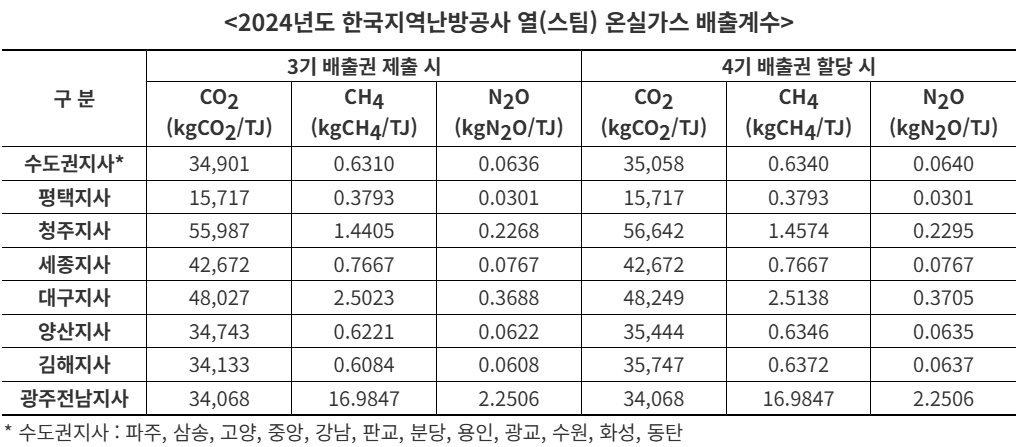
\includegraphics[width=\textwidth]{지역난방공사 온실가스 배출계수 공표 (나중에 표로 바꾸기).png}
  \caption{한국지역난방공사의 온실가스 배출계수 공포 예시 (2024년 기준)}
  \label{fig:co2_bboombboom}
\end{defaultfigure}

가스 및 등유는 2006년 이후로 개정된 바 없으며, 추후 IPCC 개정에 따라 수정 반영되어야 한다. 전기 및 지역난방의 경우 매년 공포되는 값이므로, 매년 공포되는 내용에 따라 계수가 수정 반영되어야 한다.

\subsubsection{비용}
연료별 비용 환산 계수는 표 \ref{tbl:coeff_kWh_to_cost}\와 같다. 에너지 요금 체계는 기본요금, 구간별 단가, 계절별 차등 등 다양한 요소로 구성되어 있어 단일 기준으로 정확히 산정하기는 어렵다. 따라서 복잡한 체계를 단순화하여 대표 환산계수를 적용하는 통계적 접근 방식을 사용하였다.

\begin{table}[ht]
  \caption{연료별 사용량의 요금 환산 계수}
  \label{tbl:coeff_kWh_to_cost}  
  \centering
  \begin{tabular}{cr}
    \toprule
    연료명 & 환산계수 [won/kWh] \\ \midrule
    전기 & 162.92 \\
    가스 & 78.12 \\
    등유 & 141.92 \\
    지역난방 & 94.98 \\ \bottomrule
  \end{tabular}
\end{table}

\paragraph{전기, 가스 및 등유} 매월 발간되는 KESIS 국가에너지통계 종합정보시스템에서 2024년 기준값을 참고하였다 (그림 \ref{fig:naturalgas_cost}). 전기와 가스의 경우 말단 용도별로 상이한 통계치가 제시되는데, 각 건물의 계약전력 등 세부 구분을 명확히 반영하기 어려우므로 각 용도별 값의 평균을 사용하였다. 예를 들어, 도시가스의 경우 가정용(21.4원/MJ), 일반용(21.0원/MJ), 산업용(20.8원/MJ), 업무난방용(23.6원/MJ)의 평균인 21.7원/MJ을 기준값으로 사용하였다.

\begin{defaultfigure}
  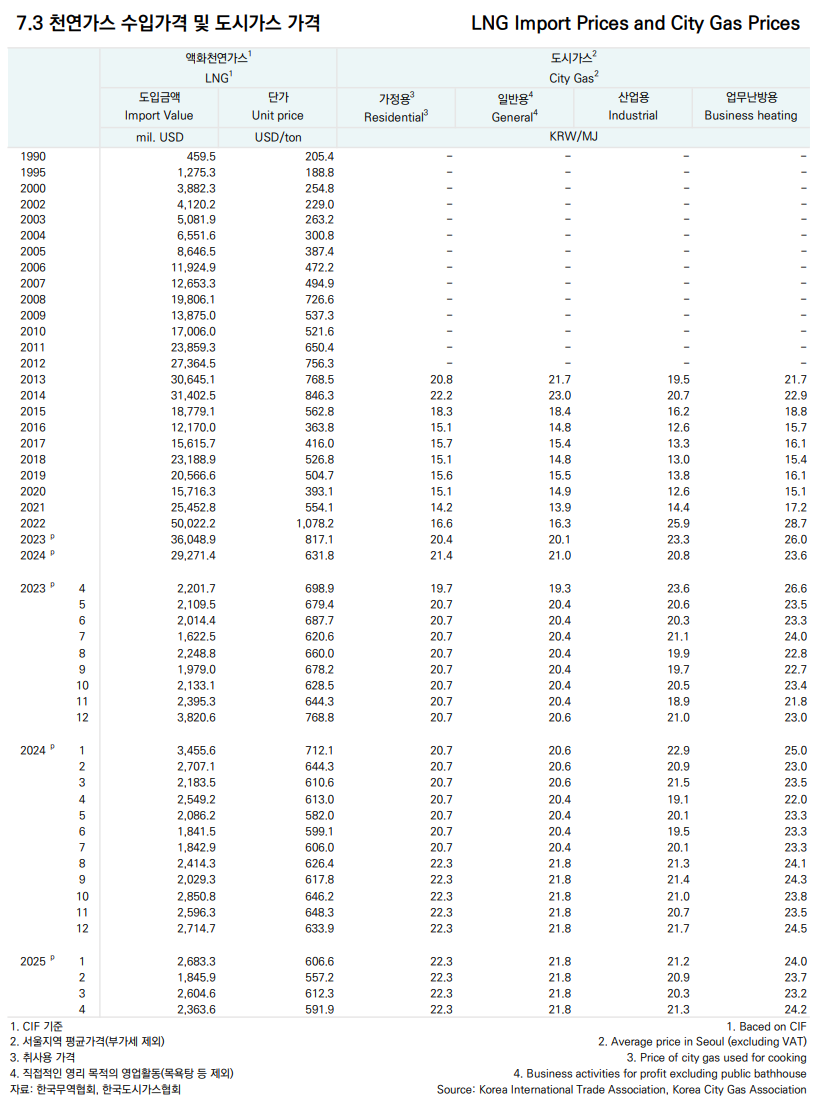
\includegraphics[width=\textwidth]{KIESIS 도시가스 가격 공표 (나중에 표로 바꾸기).png}
  \caption{KIESIS의 도시가스 가격 공포 예시 (2024년 기준)}
  \label{fig:naturalgas_cost}
\end{defaultfigure}

이 때 에너지열량 환산기준은 「에너지법 시행규칙」을 참고하였다. 연료의 발열량은 총발열량이 아닌 순발열량을 적용하는 것이 원칙이다. 이는 연소 과정에서 수분 증발 잠열 손실을 제외한 실제 이용 가능한 에너지량을 반영해야 하기 때문이다.


\paragraph{지역난방} 지역난방은 한국지역난방공사의 경영실적 공시에 판매단가를 명시하고 있다 (그림 \ref{fig:districtheating_cost}).

\begin{defaultfigure}
  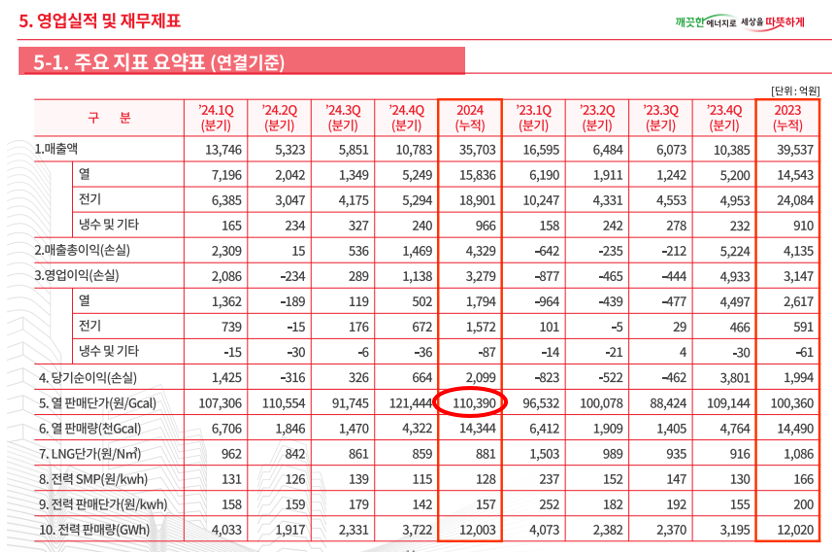
\includegraphics[width=\textwidth]{지역난방공사 운영실적 (나중에 표로 바꿔야되나).png}
  \caption{한국지역난방공사 판매단가 공시 예시 (2024년 기준)}
  \label{fig:districtheating_cost}
\end{defaultfigure}

% chap2.tex
\part{유지보수 및 신기술 적용}
\label{part:module}

% ---------------------------------------------------------------------------- %
%                                  NEW SECTION                                 %
% ---------------------------------------------------------------------------- %

\chapter{pyGRsim 모듈}

% ---------------------------------------------------------------------------- %
%                                  NEW SECTION                                 %
% ---------------------------------------------------------------------------- %

\section{pyGRsim 구조별 상세}
pyGRsim이랑 dragon이랑 launcher랑 나누어서 서술할 것임.

\subsection{pyGRsim}

\subsection{idragon}

% ---------------------------------------------------------------------------- %
%                                  NEW SECTION                                 %
% ---------------------------------------------------------------------------- %

\section{데이터 변환의 구현}
\subsection{grexcel to grjson}
...한 과정으로 이루어진다.

\subsection{grjson to GreenRetrofitModel}
...한 과정으로 이루어진다.

\subsection{GreenRetrofitModel to EnergyModel}
...한 과정으로 이루어진다.

\subsection{EnergyModel to idf}

\subsubsection{idf 기본 설정}
기본적으로 돌아가게 하기 위해서 아래 객체들을 먼저 만들어준다.

\subsubsection{DB류 객체들 내보내기}
material, construction, profile 들을 만들어준다.

\subsubsection{실재하는 객체들 하나씩 내보내기}
zone, surface, 설비같은 것들에 해당된다. 모든 EnergyModel 객체들은 다 to\_idf\_object 객체 가지고 있음. 기본적으로는 자기자신을 idfobject화 해서 계속 append하는 것이다.

\subsubsection{후처리}
...가 필요하다.

\subsubsection{ouptut 관리 등}
...가 필요하다.

% ---------------------------------------------------------------------------- %
%                                  NEW SECTION                                 %
% ---------------------------------------------------------------------------- %

\section{EnergyPlus의 실행}
외부에서 입력이 들어오면, 그림 \ref{fig:eplaunchbycode}\와 같이 EnergyPlus가 호출된다.
\begin{defaultfigure}
  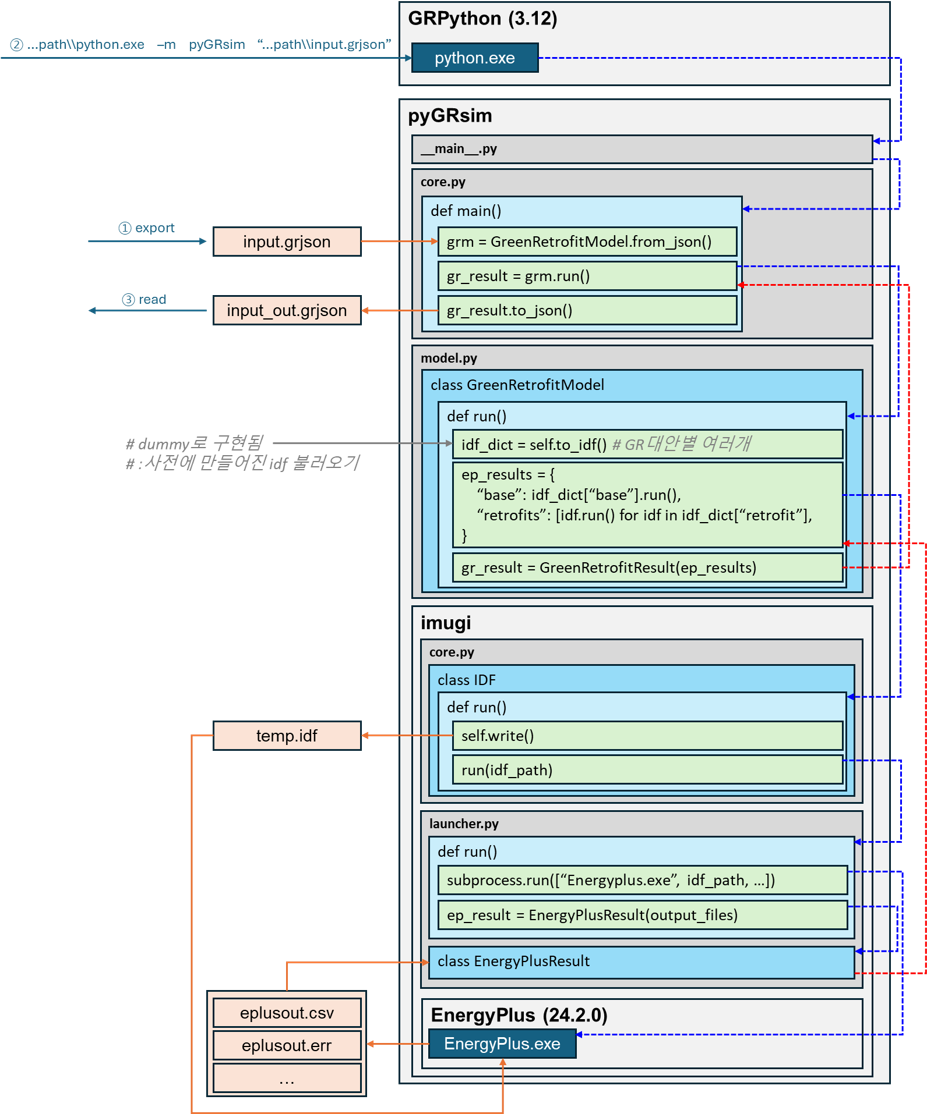
\includegraphics[height=0.99\textheight, width=\textwidth, keepaspectratio]{실행구조도.png}
  \caption{외부 호출 시 EnergyPlus launch되는 호출 흐름}
  \label{fig:eplaunchbycode}
\end{defaultfigure}

% ---------------------------------------------------------------------------- %
%                                  NEW SECTION                                 %
% ---------------------------------------------------------------------------- %

\section{예시코드}

% ---------------------------------------------------------------------------- %
%                                  NEW SECTION                                 %
% ---------------------------------------------------------------------------- %

\chapter{알고리즘의 수정과 코드의 유지보수}

\section{알고리즘의 수정 제안}

% ---------------------------------------------------------------------------- %
%                                  NEW SECTION                                 %
% ---------------------------------------------------------------------------- %

\section{기본값 변경}

% ---------------------------------------------------------------------------- %
%                                  NEW SECTION                                 %
% ---------------------------------------------------------------------------- %

\section{일반적인 코드의 유지보수}


% ---------------------------------------------------------------------------- %
%                                  NEW SECTION                                 %
% ---------------------------------------------------------------------------- %

\chapter{신기술 적용}

\section{신기술의 시뮬레이터 적용하기 위해 필요한 개념적인 과정}

% ---------------------------------------------------------------------------- %
%                                  NEW SECTION                                 %
% ---------------------------------------------------------------------------- %

\section{신기술을 본 시뮬레이터로 테스트해보는 방법}

idf에 모듈 형식으로 결합할 수 있도록 (즉, 독립적으로 추가될 수 있도록) 작성하여야 한다. 

% ---------------------------------------------------------------------------- %
%                                  NEW SECTION                                 %
% ---------------------------------------------------------------------------- %

\section{제도적으로 제출하기 위해 필요한 것}

이런 것들을 테스트하여 제출하면 평가가 가능하다.
% \nocite{*}

% --- 부록 --- 
% chap2.tex
\part{부록}
\appendix
\renewcommand{\chapterlabel}{Appendix~\thechapter}

% ---------------------------------------------------------------------------- %
%                                  BACKMATTER                                  %
% ---------------------------------------------------------------------------- %

% --- 참고문헌 ---
\backmatter
\bibliographystyle{plain}
\bibliography{_common/references}

% --- 문서 끝 ---
\end{document}
